%%%%%%%%%%%%%%%%%%%%%%%%%%%%%%%%%%%%%%%%
%% MCM/ICM LaTeX Template %%
%% 2025 MCM/ICM           %%
%%%%%%%%%%%%%%%%%%%%%%%%%%%%%%%%%%%%%%%%
\documentclass[12pt]{article}
\usepackage{geometry}
\geometry{left=1in,right=0.75in,top=1in,bottom=1in}

%%%%%%%%%%%%%%%%%%%%%%%%%%%%%%%%%%%%%%%%
% Replace ABCDEF in the next line with your chosen problem
% and replace 1111111 with your Team Control Number
\newcommand{\Problem}{C}
\newcommand{\Team}{2502406}
%%%%%%%%%%%%%%%%%%%%%%%%%%%%%%%%%%%%%%%%
\usepackage[utf8]{inputenc}
\usepackage{tocloft}
\usepackage{color}
\usepackage{booktabs}
\usepackage{listings}
\usepackage[numbers]{natbib}
\bibliographystyle{apalike}
\usepackage{verbatim}  
\usepackage{longtable}
\usepackage{enumitem}
\usepackage{amsmath}
\usepackage{bm}



\lstdefinestyle{mystyle}{
    backgroundcolor=\color{gray!10},     % Code background color is light gray
    commentstyle=\color{green!60},       % Comment style
    keywordstyle=\color{blue},           % Keyword style
    numberstyle=\tiny\color{gray},       % Line number style
    stringstyle=\color{purple},          % String style
    basicstyle=\ttfamily\footnotesize\linespread{1.2}\selectfont, % Increase line spacing
    breakatwhitespace=false,             % Break lines only at whitespace
    breaklines=true,                     % Automatic line wrapping
    captionpos=b,                        % Caption position (bottom)
    keepspaces=true,                     % Preserve spaces (helps maintain code indentation)
    numbers=left,                        % Line numbers displayed on the left
    numbersep=8pt,                       % Distance between line numbers and code
    showspaces=false,                    % Do not show spaces
    showstringspaces=false,              % Do not highlight spaces within strings
    showtabs=false,                      % Do not show tabs
    tabsize=2,                           % Number of characters a tab stop occupies
}


\usepackage{newtxtext}
\usepackage{amsmath,amssymb,amsthm}
\usepackage{newtxmath} % must come after amsXXX

\usepackage[pdftex]{graphicx}
\usepackage{xcolor}
\usepackage{fancyhdr}
\lhead{Team \Team}
\rhead{}
\cfoot{}

\newtheorem{theorem}{Theorem}
\newtheorem{corollary}[theorem]{Corollary}
\newtheorem{lemma}[theorem]{Lemma}
\newtheorem{definition}{Definition}

\renewcommand{\cftsecleader}{\bfseries\cftdotfill{\cftdotsep}}
%%%%%%%%%%%%%%%%%%%%%%%%%%%%%%%%
\begin{document}
\graphicspath{{.}}  % Place your graphic files in the same directory as your main document
\DeclareGraphicsExtensions{.pdf, .jpg, .tif, .png}
\thispagestyle{empty}
\vspace*{-16ex}
\centerline{\begin{tabular}{*3{c}}
	\parbox[t]{0.3\linewidth}{\begin{center}\textbf{Problem Chosen}\\ \Large \textcolor{red}{\Problem}\end{center}}
	& \parbox[t]{0.3\linewidth}{\begin{center}\textbf{2024\\ MCM/ICM\\ Summary Sheet}\end{center}}
	& \parbox[t]{0.3\linewidth}{\begin{center}\textbf{Team Control Number}\\ \Large \textcolor{red}{\Team}\end{center}}	\\
	\hline
\end{tabular}}
%%%%%%%%%%% Begin Summary %%%%%%%%%%%
% Enter your summary here replacing the (red) text
% Replace the text from here ...
\begin{center}
    \Large\textbf{Predict 2028 Olympics Medal Table: Hierarchical Adaptive Prediction Framework with LSTM-Attention Mechanism}
\end{center}
\begin{center}
    \large\textbf{Summary}
\end{center}

In this study, we explored the dynamics of Olympic medal predictions and the specific manifestations of the great coach effect. By leveraging historical data and advanced modeling techniques, we developed two key models: one for predicting the gold medal and overall medal counts for the 2028 Los Angeles Summer Olympics which is called \textbf{HAPF-LSTM}, and another for quantifying the impact of exceptional coaches on medal outcomes. Our analysis not only provided insights into potential medal distributions, aiding each nation's Olympic Committee in strategic adjustments but also offering investment recommendations in \textbf{great coach effect} for three countries.\\

The first model provided a detailed \textbf{hierarchical adaptive} forecast for the 2028 Olympics, identifying medal distribution patterns and performance trends among nations. By integrating historical data and \textbf{feature engineering}, we quantified characteristics like dominance, and fierceness of competitions, which came from either nation's and certain Olympic year's aspects. The model \textbf{progressively} uses the main data group by going through \textbf{random-forests-classifier} for predictions of whether will achieve a medal and then going through the regressor powered by \textbf{MLP}, with the collaboration of additional important data group. Differences in going through \textbf{various branches} mainly depend on a \textbf{timely judgment} of whether a country is competitive enough. \textbf{LSTM-Attention mechanism} is introduced to the model to drive the training and evaluation. The model offered insights into countries that are steadily competitive and those hardly having achieved any medals. These predictions not only informed audience expectations but also provided strategic guidance to national Olympic committees for refining their sports development strategies.\\

The second model, leveraging a data-driven approach, confirmed the existence of the \textbf{great coach effect} and quantified its influence on medal counts. The study highlighted the significant role that top-level coaches play in enhancing medal performance. Furthermore, it identified three additional factors, \textbf{Sports Powerhouse} , \textbf{Stable Athlete Pool} and \textbf{Historical Success} which are based on insights from relevant research, that can help determine which sporting events would benefit most from the investment in a great coach. This \textbf{quantitative analysis} highlighted the significant impact of exceptional coaching on athletic success, specifically identifying Sailing in Great Britain, Boxing in the United States, and Trampoline Gymnastics in China as key areas for improvement. \\

By integrating various methods and incorporating diverse variables, our model demonstrates robustness and stability, ensuring reliable performance even with noisy or incomplete data. Future research could build on these findings by incorporating additional variables, such as athlete development programs, technological advancements, and socio-economic factors, to further refine predictions and deepen insights. \\

\noindent \textbf{Keywords:} Olympics, medal estimation, hybrid model, Random Forest, LSTM, Attention,  MLP, great coach effect

%%%%%%%%%%% End Summary %%%%%%%%%%%

%%%%%%%%Begin Content%%%%%%%%
\clearpage
\pagestyle{fancy}
\tableofcontents
\newpage
\setcounter{page}{1}
\rhead{Page \thepage\ }
%%%%%%%% End Content %%%%%%%%%

\section{Introduction}
\subsection{Problem Background}
\quad \quad The Olympic Games represent a unique global spectacle, featuring athletes from more than 200 countries competing in more than 400 events in both the Summer and Winter Games. This prestigious multi-sport event not only showcases competition but also fosters inspiration and unity among participants and spectators worldwide \cite{grasso2015historical}.\\

During the 2024 Summer Olympics, Paris became the center of sport enthusiasts around the world. Spectators focused not only on the outcomes of individual events but also on the national rankings in the medal tally. The United States and China performed notably, each securing an equal number of gold medals, demonstrating their formidable prowess in global sports. Meanwhile, the host nation France, although ranked fifth in gold medals, secured the fourth position in total medals, suggesting that the home advantage may have positively influenced their performance. Additionally, this Olympics witnessed breakthroughs by smaller nations such as Saint Lucia and Albania, which not only won Olympic medals for the first time but also captured gold, marking significant progress in their sporting achievements. This phenomenon indicates that the Olympics not only serve as a competitive arena for sports powerhouses but also provide a platform for smaller nations to showcase their developmental strides.\\

With the progression of globalization and the rise of social media, there is an increasing focus on sports events, especially massive competitions like the Olympics \cite{CONDON19991243}. Medal predictions for the Olympics not only satisfy the curiosity of the audience but also offer substantive guidance to national Olympic committees to improve their countries' standings on the medal table. Predictions are typically based on the athletes' capabilities and past performances, yet the outcomes of the Games are often filled with uncertainties. This unpredictability not only enhances the spectacle of the competitions but also makes forecasting a challenging task.

\subsection{Restatement of the Problem}
\begin{itemize}
  \item \textbf{Question 1:} \\
  The first question can be divided into three sub-questions. The first sub-question involves predicting the medal tally for the 2028 Los Angeles Summer Olympics, including all result intervals, and analyzing which countries are likely to perform better or worse compared to 2024. The second sub-question estimates the number of countries that might win their first Olympic medals in 2028 and discusses the likelihood of these predictions. The final sub-question explores how the number and type of events influence the distribution of medals among competing nations, identifies key sports crucial to different countries and the reasons why, and assesses how the selection of events by the host nation might impact the outcomes of the games.
  \item \textbf{Question 2:} \\
  Through data analysis, investigate whether there are performance changes that can be attributed to the influence of great coaches. Please evaluate the extent of this impact on medal count. Subsequently, select three countries and analyze which sports could benefit from investing in top-level coaches, and estimate the potential effectiveness of this strategy.
  
  \item \textbf{Question 3:} \\
  Analyze the Olympic medal counts predicted by the existing model and provide unique insights to inform the national Olympic committees.
\end{itemize}

\subsection{Literature Review}
\quad \quad With the rapid development of social media and the growing aspiration of people for a higher quality of life, the Olympic Games, an ancient and prestigious sporting event, have captured unprecedented levels of global attention in the 21st century \cite{grasso2015historical}. As a result, predicting the Olympic medal counts each year has also become a focal point for audiences.\\

For each Olympic Games, a significant amount of literature provides predictions. For example, Sanchez-Fernandez et al. describe the process of predicting the distribution of Olympic medals. By analyzing the accuracy of predictions made for the 2012 London Olympics, it further predicts the medal distribution for the 2016 Rio Olympics and provides the medal rankings for each country \cite{sanchez2016olympic}. There is another study that aimed to predict the success of countries participating in the Tokyo 2020 Olympics using smart methods, including the PEST+S model and neural network modeling \cite{fazlollahi2020predicting}. Nagpal‘s team mainly discusses the status of the Olympics as a top international sporting event and uses data from the 2020 Tokyo Olympics to predict the medal counts for the 2024 Paris Olympics \cite{nagpal2023paris}. The above studies focused on predicting medal counts for the 2016 Rio Olympics, the 2020 Tokyo Olympics, and the 2024 Paris Olympics. From this, we can observe that forecasting the distribution of gold medals for each edition of the Olympic Games has become a consistent and enduring tradition. This practice reflects not only the audience’s fascination with the competitive outcomes but also the broader interest in analyzing patterns, trends, and factors that influence athletic success on the global stage \cite{grasso2015historical}. Such predictions serve as a bridge between historical performance and future expectations, enriching the Olympic experience for fans, researchers, and stakeholders alike.\\

Scelles et al. provide a wealth of recommendations on feature selection for predicting the gold medal tally in his paper. Including the population size of a country four years prior to the Olympic Games, the country's economic development, the host country effect, country regions, medal totals four years earlier and so on \cite{scelles2020forecasting}. For prediction model selection, Varagiri Shailaja's team experimented with some common algorithm including Decision Tree, KNN, Linear Regression, Random  Forest Algorithm and Bayesian Ridge Algorithm \cite{shailaja2020predictive}. Moreover, Edward M. Condon built linear regression models and neural network models and and afterwards compared them, indicating the neural network model outperformed the regression model \cite{CONDON19991243}. Christoph Schlembach proposed a socioeconomic machine learning model including Tobit model and Hurdle modeel \cite{SCHLEMBACH2022121314}. The Tobit model is a type of regression model designed to handle censored dependent variables, where the observed values are either partially or entirely limited by a threshold (e.g., non-negative variables like income or scores) \cite{amemiya1984tobit}. It is commonly used in cases where the dependent variable is restricted in range, allowing for the estimation of relationships while accounting for the censoring effect, providing more accurate and meaningful results than standard linear regression \cite{mcdonald1980uses}. The above literature on variable selection and model choice provides a solid foundation for our work.

\subsection{Our Work}
\quad \quad We began by collecting relevant literature on the topic, learning from previous research on medal prediction. We are initiating the processes of data pre-processing and data analysis. After that, we proceeded to build our models.\\ 

The first model, Hierarchical Adaptive Prediction Framework Driven by LSTM-Attention Mechanism (HAPF-LSTM), is designed to predict the gold and overall medals for 2028 Olympics. We analyzed data from two perspectives: the characteristics of participating countries and the features of events in each Olympic year. Participating-nation-factors such as host nation status, athlete quality, and event dominance, as well as certain-Olympic-year-features like the competition intensity and the number of events, were integrated into different parts of the model for prediction. This approach achieved strong predictive performance. To account for differences between countries, we designed specialized model branches for those with low medal prospects and consistently top-ranked nations, allowing for tailored prediction strategies. Additionally, we applied the 'LSTM $+$ Attention' mechanism to capture temporal features and fine-tuned the model with the Adam optimizer, leading to satisfactory results.\\

The second model is capable of accurately reflecting the great coach effect on the medal standings. We identified three additional great coaches and analyzed the changes in medal counts before and after the five coaches began coaching and the local highest value in medal count during the coaching period. These data allowed us to assess the impact of these exceptional coaches on specific events across various countries. Additionally, by examining relevant research, we identified three other critical factors that significantly influence the effectiveness and value of investing in a coach for a particular sport: Sports Powerhouse, Stable Athlete Pool and Historical Success. Using the three features we filtered the most suitable sports of coach investment.\\

 Evaluation, strengths and weaknesses of the proposed model are discussed afterward. All source codes and the prediction medal table for 2028 Los Angeles, USA summer Olympics are attached to the Appendix. 

\section{General Assumptions and Notations}

\subsection{Assumptions}

\begin{enumerate}[itemsep=0pt, topsep=0pt]
    \item It is assumed that the collected data is authentic and reliable, with no instances of fabrication.
    \item It is assumed that athletes from all countries compete with integrity, without resorting to substances such as doping or high-tech aids beyond the rules (such as specially designed clothing or sports equipment), and that no cheating occurs.
    \item For sports involving referees, it is assumed that referees are fair and impartial, and there will be no intentional misjudgments, omissions, or favoritism.
    \item The possibility of major sporting nations refusing to participate in the Olympics for various reasons is not considered, nor is the absence of athletes due to injuries or other reasons.
    \item The impact of the International Olympic Committee's temporary changes to the competition rules on the performance of athletes is not considered.
\end{enumerate}

\subsection{Notations}
\begin{table}[h!]
\centering 
\renewcommand{\arraystretch}{1.5}
\begin{tabular}{cc} 
\toprule
Symbol & Description \\
\midrule
$TS_{i,j}$ & Total score of the $i^{\text{th}}$ country in the $j^{\text{th}}$ sport.\\
$S_{i,j}$ & Score rate of the $i^{\text{th}}$ country in the $j^{\text{th}}$ sport.\\
$a_{i,j}$ & Number of athlete of the $i^{\text{th}}$ country in the $j^{\text{th}}$ sport.\\
$Q_{i,j}$ & Athlete quality of the $i^{\text{th}}$ country in the $j^{\text{th}}$ sport. \\
$m_j$ & Number of events in the $j^{\text{th}}$ sport\\
$n_{Gold}$ & Number of gold medals \\
$n_{Silver}$ & Number of silver medals \\
$n_{Bronze}$ & Number of bronze medals \\
$P_{1s}$ & Score achieved by the team under the coach's leadership during Period 1 \\
$\Delta_{pre1}$ & Difference in score compared to the previous term \\
$\Delta_{max1}$ & Difference in score compared to the best performance among the previous three terms \\
$P_{2s}$ & Score achieved by the team under the coach's leadership during Period 2 \\
$\Delta_{pre2}$& Difference in score compared to the previous term \\
$\Delta_{max2}$ & Difference in score compared to the best performance among the previous three terms \\
$\delta$ & If it is a team event\\
\bottomrule
\end{tabular}
\label{tab:symbols_descriptions}
\end{table}

\section{Data Preprocessing and Analysis}
\subsection{Data Preprocessing}

\quad \quad After reviewing the provided dataset, we find that only one file which is called summerOly\_programs.csv contains some missing or anomalous data points. First, we address the missing values by replacing all of them with a question mark. Following that, we handle outliers, which includes removing irrelevant information, deleting columns related to competitions outside the Olympic cycle, and eliminating rows with incomplete data. In the 'Sports Governing Body' column, replace question marks with NULL, and then substitute any other occurrences of question mark with the number 0. After completing these operations, we recalculate the totals for events, disciplines, and sports and correct the data accordingly.\\

After addressing outliers and missing values, we further consolidated the data. First, we removed the years from the summerOly\_hosts.csv file for which the Olympic Games were not successfully held. Next, we delete the contents within parentheses to standardize the format of the host location names and use regular expressions to extract text and ensure there are no extra spaces. Finally, we used pandas to split the city and country names, then linked these with the summerOly\_medal\_counts.csv and summerOly\_athletes.csv tables to obtain the final clean and usable data.\\

Furthermore, there are 18 kinds of sports events that have not occurred in the past 10 years which are then deemed outdated and are therefore all removed. For example, Art competition, Alpinism, Aeronautics and so on. The naming convention of the 'sport' column in the 'athletes' table should be consistent with that in the 'programs' table.

\subsection{Data Analysis}

\quad \quad Through data analysis and visualization, we have created the two charts above to illustrate the trends in event count changes in sports over the years. We removed events with a count of 0, indicating that these sports were not successfully held. \\

Figure \ref{fig1} offers a macro view of how the number of events for various sports at the Summer Olympics has evolved from 1896 to 2024. It is evident that certain events experienced significant growth in specific years, particularly newly introduced or developing sports, which reflect a more diversified trend. The scattered points and line segments signify that these events were short-lived and did not continue to appear in subsequent Olympic Games. \\

\begin{figure}[h] 
\centering
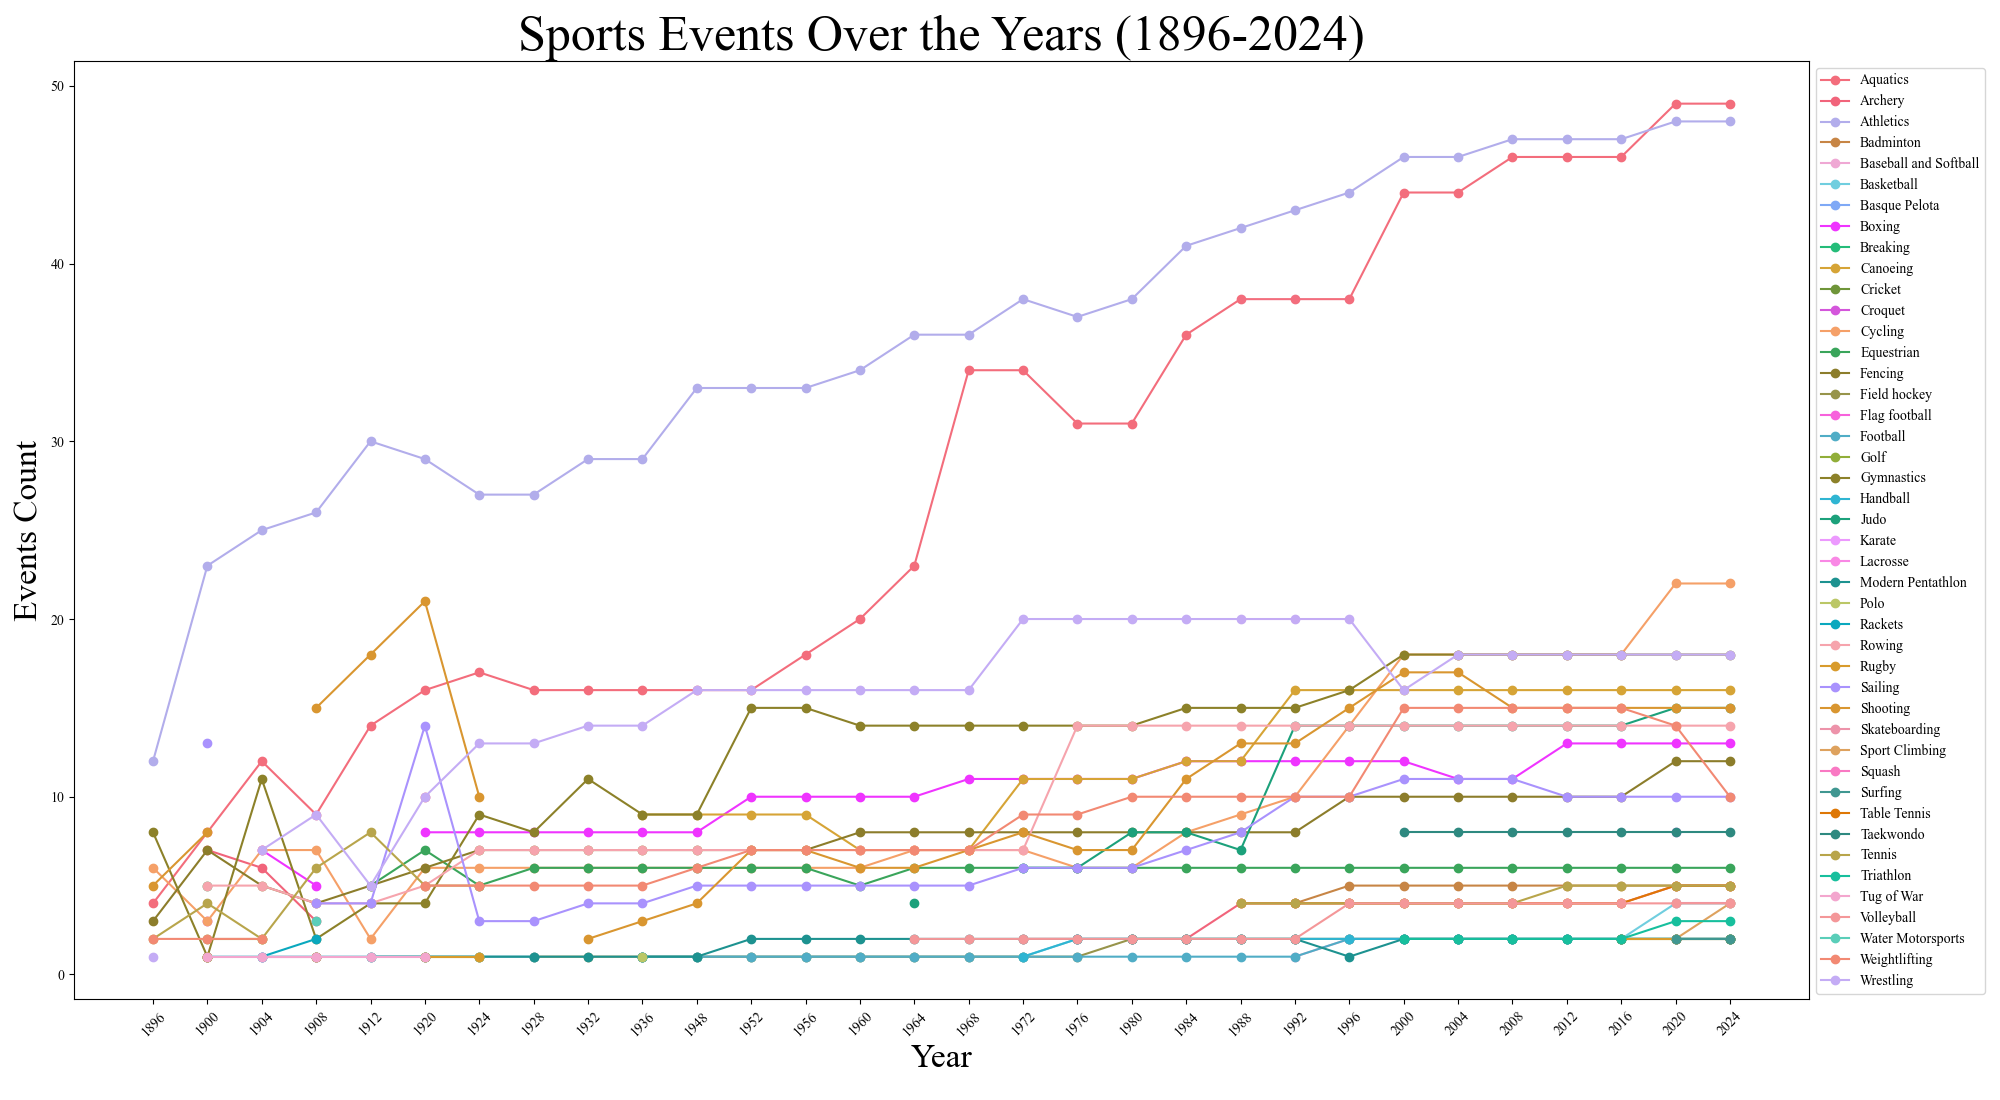
\includegraphics[width=14cm]{figure/Sports Events Over the Years (1896-2024).png}
\caption{Sports Events Overview for The Last 30 Summer Olympic Games} \label{fig1}
\end{figure}

\begin{figure}[h]
	\begin{minipage}[b]{0.5\textwidth}
		\centering
		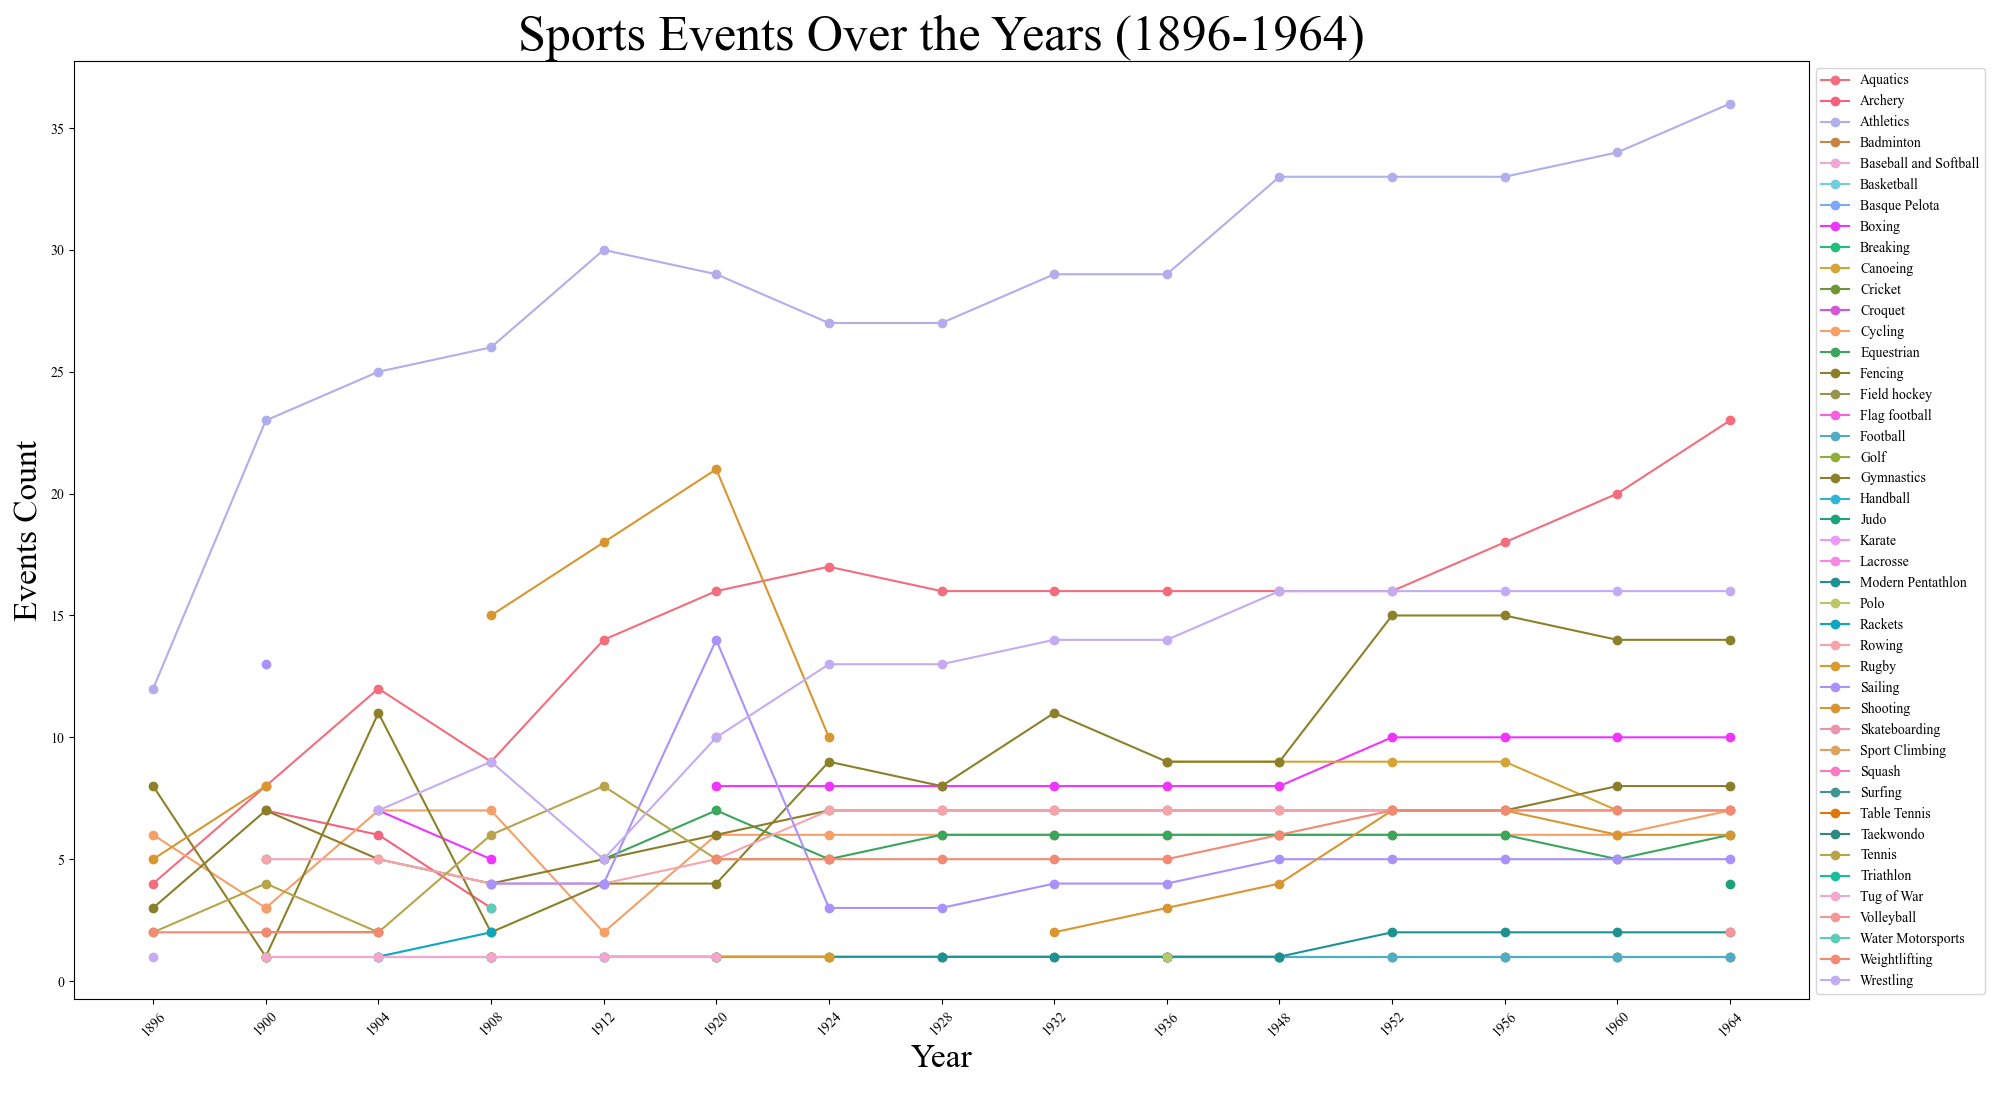
\includegraphics[width=1\textwidth]{figure/Sports Events Over the Years (1896-1964).png}
	\end{minipage}
	\begin{minipage}[b]{0.5\textwidth}
		\centering
		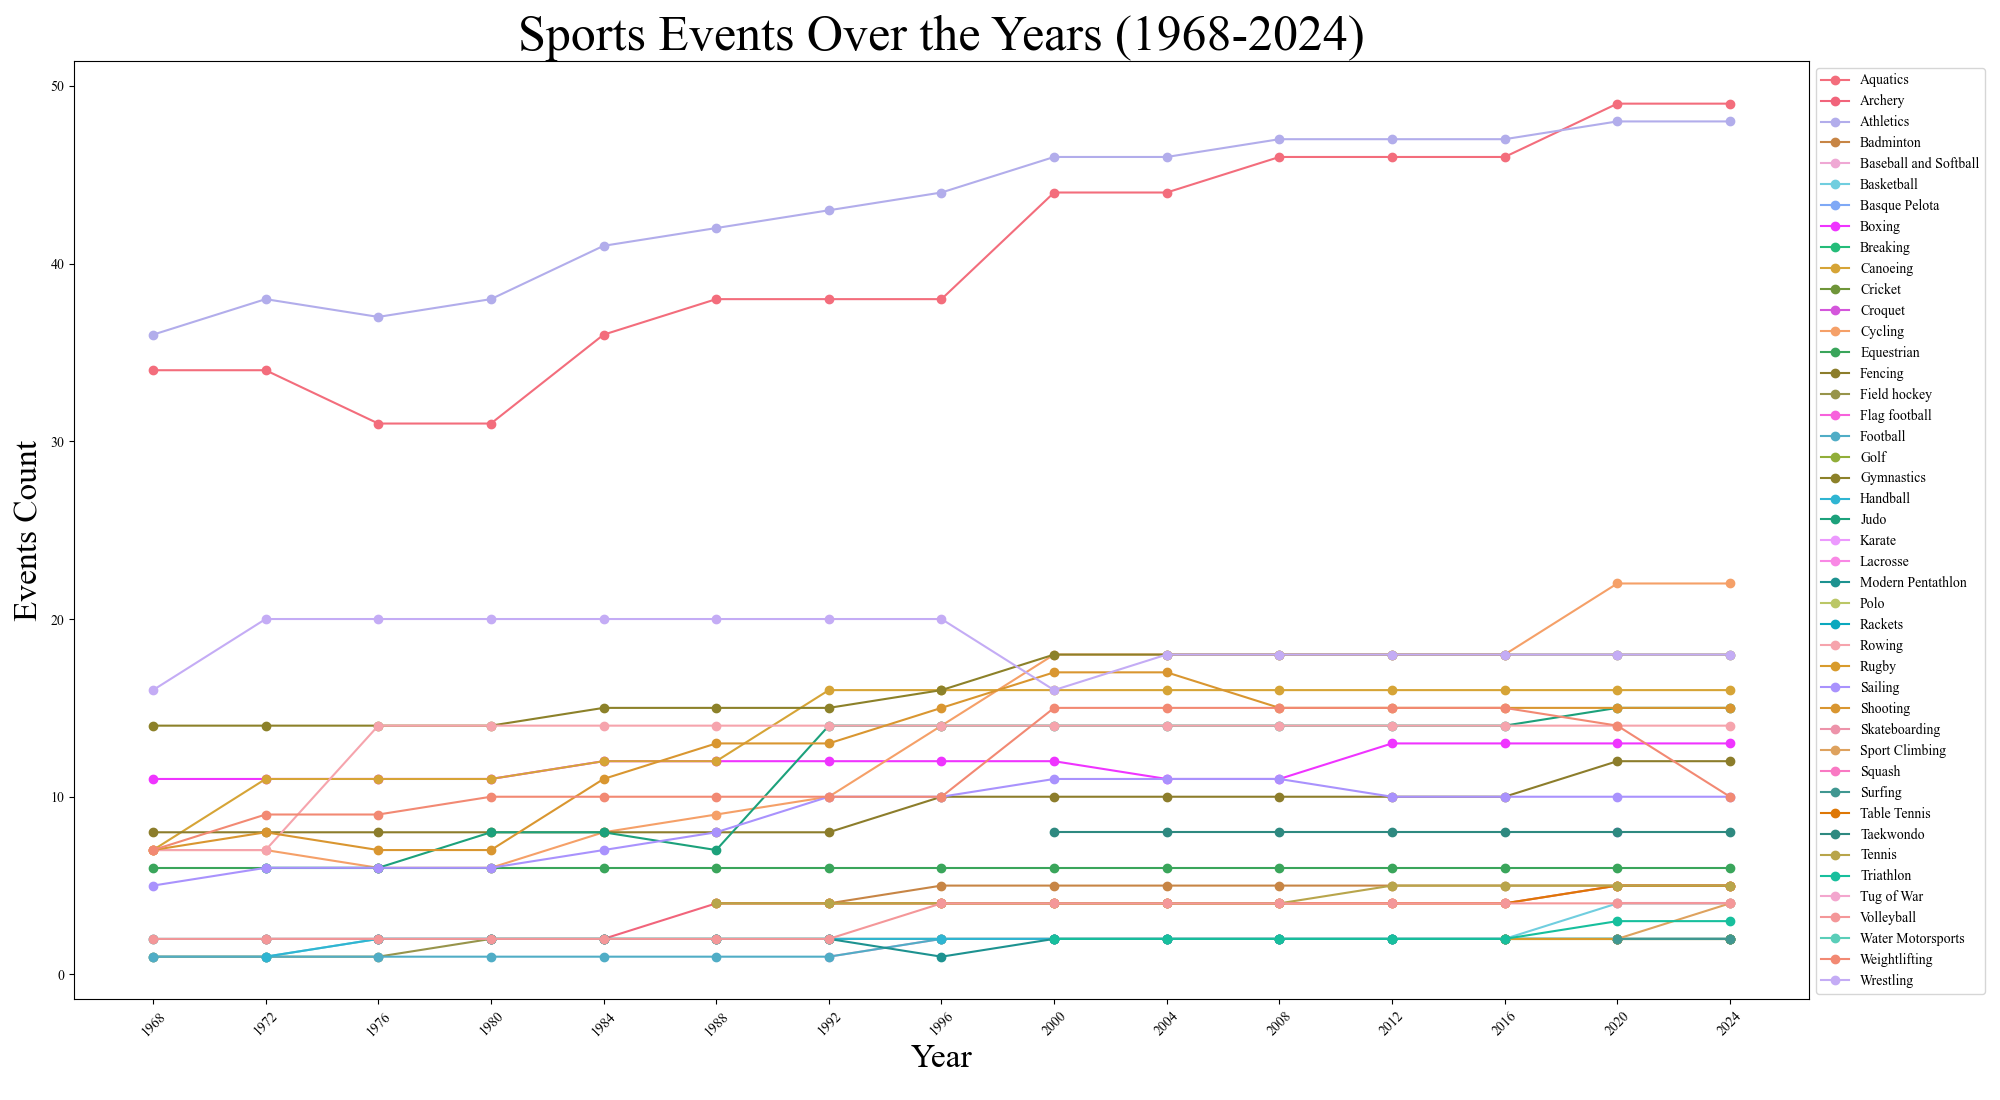
\includegraphics[width=1\textwidth]{figure/Sports Events Over the Years (1968-2024).png}
	\end{minipage}
	\caption{Comparison of Sports Events Count between 1896-1964 and 1968-2024}\label{fig2}
\end{figure}

Figure \ref{fig2} compares the event count changes from the first 15 editions of the Olympics (1896-1964) with those from 1968 to 2024. It is clear that the first 15 editions showed more fluctuation in event numbers, suggesting that the selection of sports was still in development. In contrast, the number of events in the subsequent 15 editions became more stable, indicating that the Olympic Games had reached a more mature stage. So, we brought only the second half of the Olympic years into analysis and prediction.\\

To explore the hosting effect, we examined changes in the event list based on different hosts and whether these align with the host's dominant sports. We also analyzed performance fluctuations when a country is the host, considering current, past, and future hosting scenarios.We subsequently randomly selected a year and the corresponding host country (1908, UK) and conducted a data visualization analysis of the host effect. Finally, we obtained the following bar chart.\\

\begin{figure}[h] 
\centering
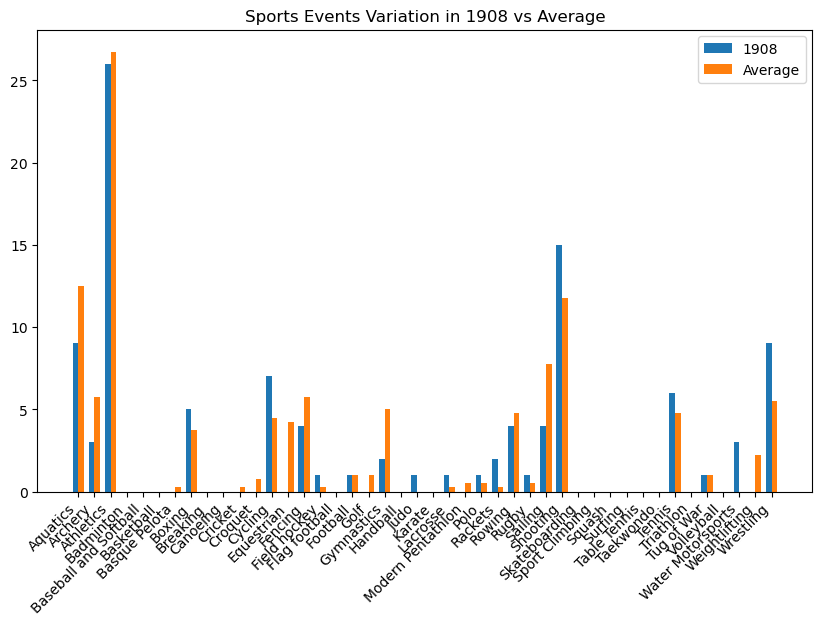
\includegraphics[width=12cm]{figure/sport_events_variation_1908.png.png}
\caption{Visualization of the Hosting-Effect} \label{fig3}
\end{figure}

The chart shows a comparison between the number of sports events in 1908 and the average number. The horizontal axis lists different sports, and the vertical axis represents the number of events. The blue bars represent the data from 1908, while the orange bars represent the average. From the chart, it can be seen that the number of events for certain sports in 1908 was significantly higher than the average, such as athletics and cycling, while for other sports it was lower than the average, such as baseball and basketball. This chart explains the distribution of sports events when the UK was the host in 1908, and the differences in the distribution of sports events on average when other countries were hosts. Upon further observation, we find that the host country does have some influence on the selection of sports events.\\


The Fourier Transform Distance is a metric method based on Fourier transformation to measure the similarity or difference between two images. The Shape Based Distance, on the other hand, assesses the similarity or difference between two objects or shapes by comparing their geometric structures. As shown in the table, we can observe the Fourier Transform Distance and Shape Based Distance data for each Olympic host country from 1896 to 2032. By analyzing these data, we can derive a coefficient table of change to reflect the trends of variation for each year. For instance, when Belgium (BEL) was the host in 1920, its Fourier Transform Distance was 117.1523775, and its Shape Based Distance was 18.13025706, indicating a significant change in the distribution of sports events compared to the average. Similarly, when Japan (JPN) was the host in 2020, its Fourier Transform Distance was 72.37198119, and its Shape Based Distance was 11.45689952, also showing a marked difference compared to the average. These data can help us understand the impact of different countries as hosts on the distribution of Olympic sports events and the trends of change between different years.

\begin{longtable}{|c|c|c|c|}
\caption{Table of Fourier Transforms and Shape-Based Distances for Different Years and Countries}\\
\hline
\textbf{Year} & \textbf{NOC} & \textbf{Fourier Transform} & \textbf{Shape Based Distance} \\
\hline
\endfirsthead
\hline
\textbf{Year} & \textbf{NOC} & \textbf{Fourier Transform} & \textbf{Shape Based Distance} \\
\hline
\endhead
\hline
\endfoot
1896 & GRE & 12.44897663 & 2.551577259 \\
1900 & FRA & 83.26921768 & 13.05903229 \\
1904 & USA & 73.66071638 & 11.67650102 \\
1908 & GBR & 41.39282408 & 6.841051889 \\
1912 & SWE & 51.4455513 & 8.341526382 \\
1920 & BEL & 117.1523775 & 18.13025706 \\
1924 & FRA & 30.2210292 & 5.095189278 \\
1928 & NED & 3.015353154 & 0.931077955 \\
1932 & USA & 11.33551053 & 3.295729732 \\
1936 & GER & 27.45071305 & 4.452446289 \\
1948 & GBR & 17.64138247 & 2.98867595 \\
1952 & FIN & 23.70182931 & 4.133668247 \\
1956 & AUS & 13.7343408 & 2.582847666 \\
1960 & ITA & 2.542094369 & 0.872093177 \\
1964 & JPN & 14.84975411 & 2.667966737 \\
1968 & MEX & 42.7871375 & 7.042558737 \\
1972 & FRG & 34.78965986 & 5.577291953 \\
1976 & CAN & 21.88883168 & 3.855519899 \\
1980 & URS & 11.6411997 & 2.222258114 \\
1984 & USA & 10.98803475 & 2.21474652 \\
1988 & KOR & 23.57418575 & 4.11547974 \\
1992 & ESP & 26.77025262 & 4.347124447 \\
1996 & USA & 18.67467862 & 3.142705704 \\
2000 & AUS & 41.075838 & 6.519716669 \\
2004 & GRE & 17.4431855 & 2.960624485 \\
2008 & CHN & 7.51287561 & 1.742737543 \\
2012 & GBR & 4.764737058 & 1.290237613 \\
2016 & BRA & 10.51872984 & 1.968057019 \\
2020 & JPN & 72.37198119 & 11.45689952 \\
2024 & FRA & 30.59058187 & 5.222303253 \\
2028 & USA &  &  \\
2032 & AUS &  &  \\
\hline
\end{longtable}


\section{HAPF-LSTM: Hierarchical Adaptive Prediction Framework Driven by LSTM-Attention Mechanism}
\subsection{Feature Selection}
\quad \quad According to the requirements, only the provided data sets are available for our training and estimation. Due to the lack of consecutive data and the limited amount of resources, we had to make great efforts on characteristic selection and engineering. In our work, we investigated these data sets in two aspects, participating nations and the Olympic year itself. Both obvious and strenuous features are included.

\subsubsection{Feature for Participating Nation}
\textbf{A) Typical-strenuous-feature: Total Score, Score Rate and Athlete Quality}\\

The total score \(TS_{i,j}\) for \(i^{th} \) country in \(j^{th} \) sport event is determined by the number of medals there, with gold medals worth 3 points, silver medals worth 2 points, bronze medals worth 1 point, and no medal earns 0 points. One special sport event is expressed by the following equation:

\begin{equation}\label{eq2}
TS_j = \sum\limits_{i} 3 \times n_{Gold,i,j} + 2 \times n_{Silver,i,j} + n_{Bronze,i,j}
\end{equation}

The score rate \(S_{i,j}\) for a country in such a specific kind of sport is calculated by dividing the total score \(TS_{i,j}\) by the total number of events under such \(j^{th} \) sport \(m_j\) that the country participated in during the year. This score is then multiplied by 6 to standardize the score to a range that reflects the relative dominance level of the country. The formula is as follows:

\begin{equation}\label{eq3}
    S_{i,j} = \frac{TS_{i,j}}{m_j \times 6}
\end{equation}

This score rate provides an effective metric to assess the country's overall performance in such a specific sport over the year. It normalizes the performance, accounting for the number of events participated in, and gives an insight into how well the country performed relative to others. Similarly, the athlete quality $ Q_{i,j} $ for a certain country is quantified as the total score achieved by \(i^{th} \) country and their amount of athletes $ a_{i,j} $ participating in that \(j^{th} \) sport, with the equation:

\begin{equation}\label{eq3}
    Q_{i,j} = \frac{TS_{i,j}}{a_{i,j}}
\end{equation}

\noindent \textbf{B) Typical-obvious-feature: Host-nation Status}\\

First, we observed that there is a certain degree of overlap between the additional events over the years and the host country's advantageous events (taking 1920 as an example). We speculate that the host nation's advantageous events may have some correlation with the prediction of the number of competition events. By calculating the Score\_Rated\_Sum and then expressing it as a weighted average of the Score\_Rated\_Sum for the country in the two previous Olympic Games, we represent the host country's advantageous events.\\

Next, when determining the coefficient of a country relative to its most recent host year, the relationship between the current year and the year when the country last hosted the Olympics must be considered. The specific rules are as follows:

\begin{itemize}
    \item If the current year is the year when the country hosted the Olympics, the coefficient is 3.
    \item If the current year is the year immediately preceding or following the year when the country hosted the Olympics, for example, one year before or after the host year, the coefficient is 2.
    \item If the current year is two years before or after the year when the country hosted the Olympics, for example, two years before or after the host year, the coefficient is 1.
    \item If the current year does not fall into any of the above categories, the coefficient is 0.
\end{itemize}

This coefficient system is designed to reflect the unique advantages and preparation levels associated with hosting the Olympic Games. Hosting the Olympics provides a country with significant benefits, including enhanced infrastructure, improved training facilities, and increased public support for sports. These factors contribute to better performance in the years surrounding the host year. The coefficient system acknowledges these advantages by assigning larger values to years closer to the host year, thereby providing a more accurate representation of a country's competitive level during these periods.

\subsubsection{Feature for certain Olympic year}

\quad \quad Similarly, a certain Olympic year always has its special attributes. As demonstrated above, we can notice that there always exists a relationship between the host's dominating sports and the increment in the number of corresponding sports events. We specially picked out features like the increment of participating countries $ \bm{w_1} $, athlete $ \bm{w_2} $, number of events $ \bm{w_3} $. And then quantified $ \bm{w_4} $, which indicates the Intensity of competition to some extent, by the following formula:

\begin{equation}\label{eq3}
    w_4 = \frac{0.2\times w_1 + 0.8 \times w_2}{w_3}
\end{equation}

\subsubsection{Features Overview}

\quad \quad We divide the countries into those with strong sports capabilities and those with weak sports capabilities. A country is considered to have strong sports capabilities if its score\_rate\_sum is in the top 10\% of all countries, while a country is considered to have weak sports capabilities if its cumulative number of participants ranks in the bottom 20\% of all countries. 

\begin{table}[h]
\caption{Variable Descriptions in Model 1}
\centering
\begin{tabular}{@{}lll@{}}
\toprule
\textbf{Variable} & \textbf{Type} & \textbf{Description} \\ \midrule
$v_1$ & INT & Whether be host country \\
$v_2$ & LIST & Predicted number of gold medals in this edition \\
$v_3$ & LIST & Total Score, $ [TS_{i,1}, TS_{i,2},...,TS_{i,j},... ] $ \\
$v_4$ & LIST & Score Rate, $ [S_{i,1}, S_{i,2},...,S_{i,j},... ] $ \\
$v_5$ & LIST & Number of participating athletes $ [a_{i,1}, a_{i,2},...,a_{i,j},... ] $ \\
$v_6$ & INT & Number of gold medals in the last edition \\
$v_7$ & INT & Coefficient of a country relative to its most recent host year \\
$v_8$ & LIST & Athlete quality $ [Q_{i,1}, Q_{i,2},...,Q_{i,j},... ] $ \\
$v_3^{sum}$ & INT & Sum of $v3$ \\
$v_4^{sum}$ & INT & Sum of $v4$ \\
$v_5^{sum}$ & INT & Sum of $v5$ \\
$v_8^{sum}$ & INT & Sum of $v8$ \\ \midrule
$w_1$ & LIST & Increase in participating countries $ [w_{1,1}, w_{1,2},...,w_{1,j},... ] $\\
$w_2$ & LIST & Increase in participating athletes $ [w_{2,1}, w_{2,2},...,w_{2,j},... ] $ \\
$w_3$ & LIST & Increase in events $ [w_{3,1}, w_{3,2},...,w_{3,j},... ] $ \\
$w_4$ & LIST & $\frac{0.2w_1+0.8w_2}{w_3}$ \\
$w_3^{sum}$ & INT & Sum of $w3$ \\
$w_4^{sum}$ & INT & Sum of $w4$ \\\midrule
$\lambda$ & INT & Small country coefficient \\
$\mu$ & INT & Large country coefficient \\\bottomrule
\end{tabular}
\label{tab:variable_descriptions}
\end{table}

The table shows all the variables we have considered, some of which were not ultimately included in the model training for various reasons. For example, the utilization of gold medal counts (a principle that applies analogously to other types of medal) for the direct prediction of current gold medal totals may engender overfitting, thereby leading to an excessive reliance on the extrapolation of present medal counts. In the context of forecasting medal counts for the year 2028, an initial approach that employs a univariate model to predict the gold medal tally could result in an overemphasis on the outcomes derived from such a simplified forecast. This methodology may not adequately capture the complexity of the underlying factors that influence medal counts and thus may not produce robust predictions. This is one of the main reasons why we ultimately chose not to include the variable $ \bm{v_2} $ as input for our model. Another example is that to accurately reflect the competitive level of each event, the change in the number of participating countries may not be as representative as the change in the number of individual athletes. This is because the latter metric can provide a more nuanced indicator of competitive intensity, as it accounts for the increased level of participation at the athlete level. That is the reason why we finally deleted $ \bm{w_1} $.\\

After that, we categorized all the variables, and the classification table is shown below:

\begin{table}[h]
\caption{Freature Group}
\centering
\begin{tabular}{|c|c|}
\hline
\textbf{Group Name} & \textbf{Detail}\\\hline
\textbf{f\_a} & $v_5^{sum}$,$v_8^{sum}$,$ \bm{v}_8 \cdot \bm{w}_4 $, \\ \hline
\textbf{f\_b} & $v_1$,$v_6$,$v_7$,$v_3^{sum}$,$v_5^{sum}$,$v_8^{sum}$,$ \bm{v_3}\cdot \bm{v_4}$
\\ \hline
\end{tabular}
\label{tab:variable_descriptions}
\end{table}

\subsection{Main body of HAPF-LSTM}

\subsubsection{Overview}

\quad \quad Based on the idea of classification and discussion, we have constructed a multi-level distributed medal prediction model. The flowchart provides the overview of the medal prediction model. Within the LSTM-Attention model, it first determines whether a country is a small country. If it is a small country, then all variables along with variable f\_a are used by the classifier to judge whether it has won an award; if it is not a small country, then all variables are directly used to judge whether it has won an award. The next step is to determine whether it is a large country; if it is not a large country, then after adding parameter f\_b, it enters the regressor to predict the outcome; if it is a large country, then after reading parameter f\_b, it enters a two-layer regressor, and finally outputs the result.

\begin{figure}[h] 
\centering
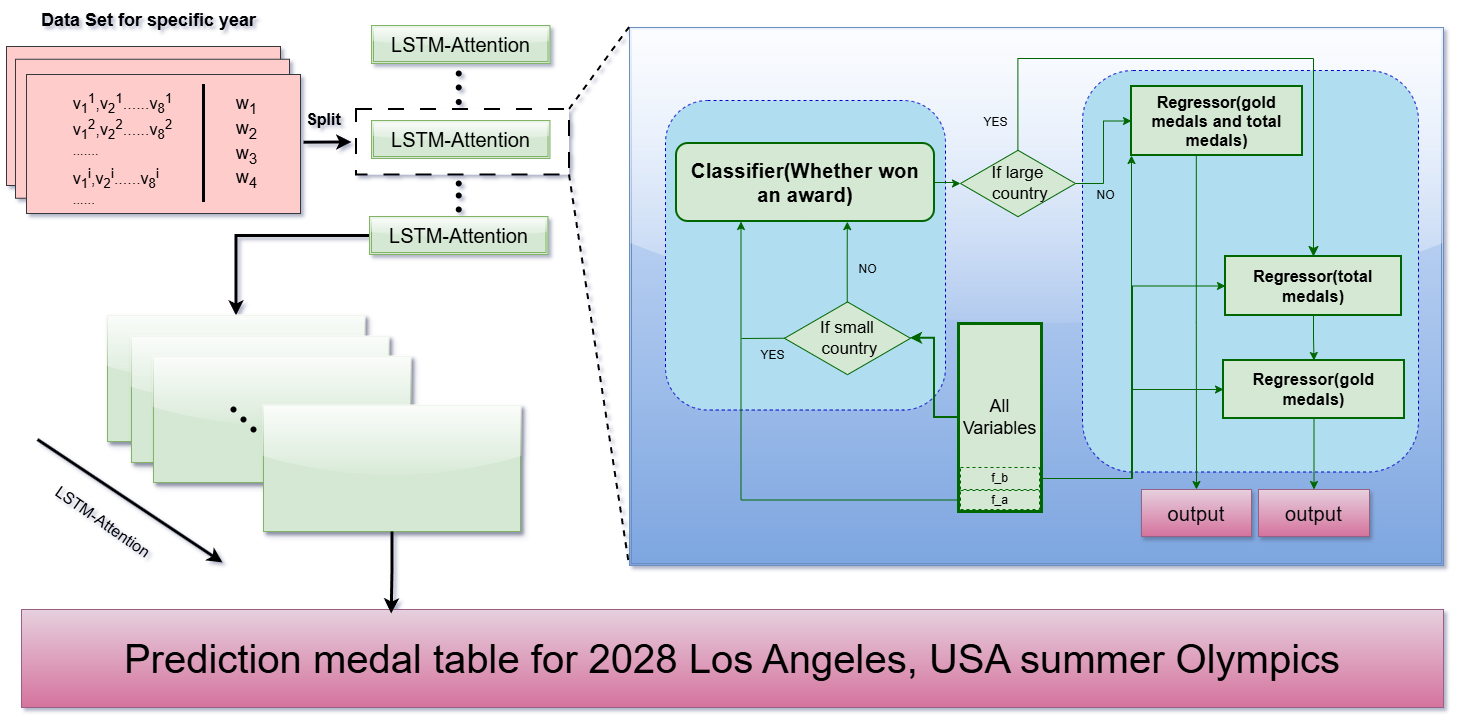
\includegraphics[width=17cm]{figure/model1.png}
\end{figure}

\subsubsection{Data Grouping and engineering}
\quad \quad To make full use of the features we sorted out previously, very careful processing must be applied, to dig the potential hint hidden behind.\\

 For $ v_1 $, there exists obvious evidence in real life demonstrating the relationship between being the host and the changes of their medal table eventually. But comparatively, the feature of the gold medal achievement list should not be utilized, as containing too much information which might cause overfitting to this feature only. For that reason, we decided to eliminate $ \bm{v_2} $ from our postselection list. However, other lists like total score and score rate, indicating the country's dominance or medal-winning ability, are important while having less possibility of causing overfitting. Also, the list of participating athletes in various events is also considerable, as well as the total amount of gold medals previously and the years away from being a host. Additionally, the inherent attributes of the certain Olympic year should also be taken into consideration. We especially picked out $ \bm{w_1} $, $ \bm{w_2} $, $ \bm{w_3} $ and calculated $ \bm{w_4} $ manually, where all of them might take some effect in the final medal board.\\

The whole group of selected features should be taken into consideration as the mainstream, and we selected some features that some small countries might have as main characteristics, or in other words, it may be difficult for them to steadily fetch medal in competitions, leading to valueless variables like the record of gold medal amounts. The group of features we selected for small countries especially the sum of participants, the total quality of athletes, and the dot product of the array of athlete quality and fierceness of sports events of this certain year.\\

The dot product combines the features of the country and of a certain year tightly and independently, without being disturbed by data from other sports events, to minimize the cross-influence among them, while also simplifying the process of linking two parts of features repeatedly. 
Similarly, two potentially valuable feature groups are identified through manual selection, consisting of individual features as well as the dot products of investigated features.\\


\subsubsection{Core Inner Structure: Hierarchical Adaptive Prediction Framework}

\quad \quad Our model has three processes in our framework: judging if winning at least a medal or not, predicting how many medals a country would win, and also how many gold medals as well. This hierarchically designed progressive model will overcome the task step by step, with full consideration of preconditions. Which might be helpful in maintaining robustness and making it more interpretable. As a result, we designed our framework from a classifier to two regressors forward,  with the timely adjustment from Adam Optimizer.\\

To cater to different prediction strategies for countries with various 
ranks of historical medal winning. We split the countries into three groups: big countries who have the sum of score rate over sports in the top 10\%, while small countries are those whose accumulated participants are in the last 20\%. During prediction, big countries might have a steady trend of winning medals and even gold medals, so we may need to lay even heavier weight on their own feature groups, which are features b and c. We first designed feature c with $ \bm{v_2} $, which was not included in feature b but was eliminated halfway, so we now take feature b as an additional feature group for big countries twice when estimating during the first and second regressors. For countries neither being big countries, they would have only one regressor that predicts the amount of gold and total medals together, with feature b as an additional feature group as well.\\ 

After determining our framework structure, we then look into the model we choose. We first utilized random forest only for our prediction framework, because according to previous experience, random forests have a good performance on the classifier especially when the feature has sufficient amount and variation. In order to fix the amount of decision-making trees, we drew the learning curve for all three layers as below. The result demonstrated that 200 would be adequate.\\

\begin{figure}[h]
	\begin{minipage}[b]{0.33\textwidth}
		\centering
		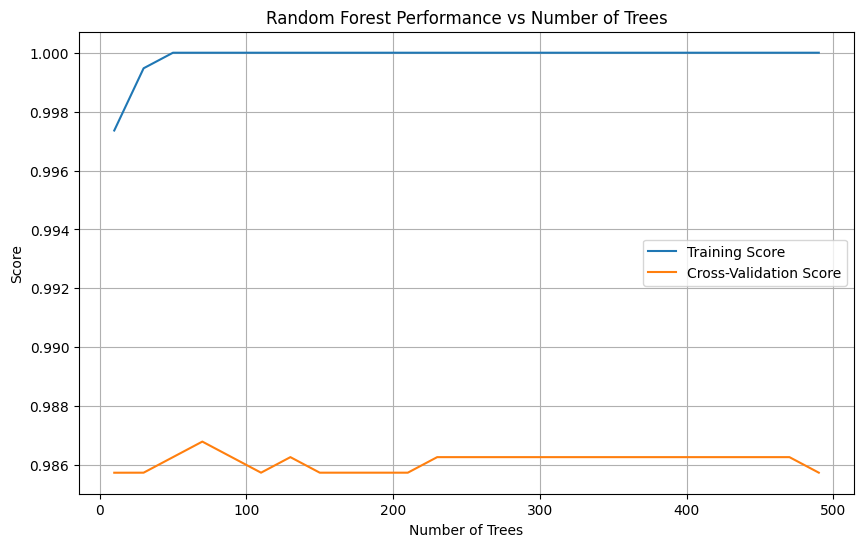
\includegraphics[width=1\textwidth]{figure/random_forest.png}
	\end{minipage}
	\begin{minipage}[b]{0.33\textwidth}
		\centering
		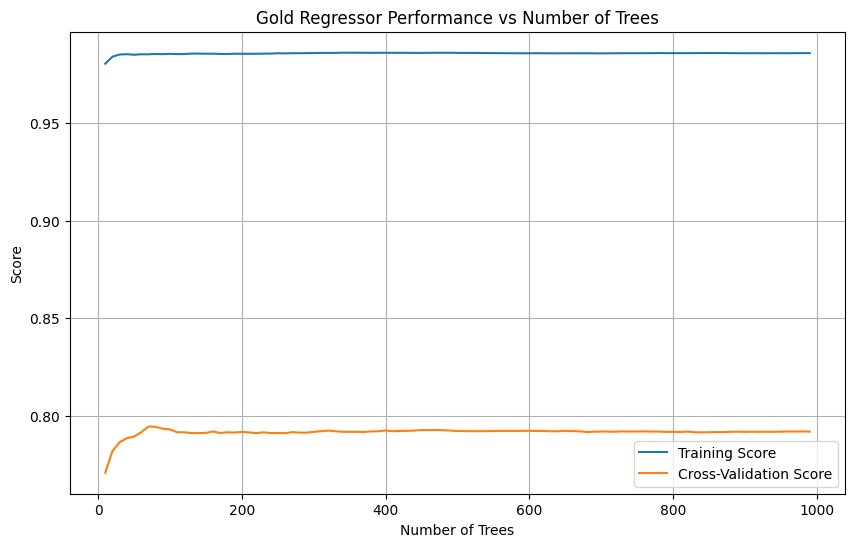
\includegraphics[width=1\textwidth]{figure/random_forest_gold_medal.png}
	\end{minipage}
    \begin{minipage}[b]{0.33\textwidth}
		\centering
		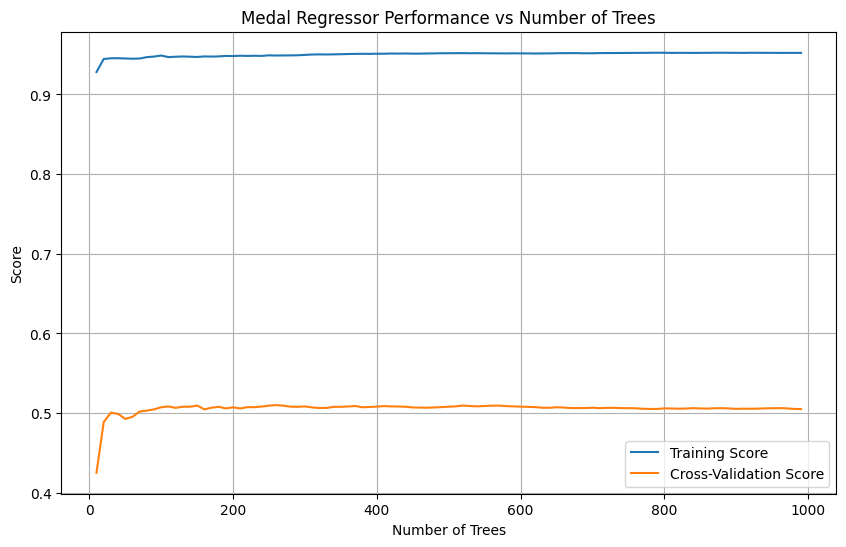
\includegraphics[width=1\textwidth]{figure/random_forest_total_meadl.png}
	\end{minipage}
	\caption{Random Forest Performance}
\end{figure}

The three tables demonstrate the performance of the Random Forest algorithm. As we can see, both the training score and the cross-validation score gradually increase and stabilize as the number of trees increases. When the number of trees reaches around 100, the model's performance is nearly optimal, and further increases in the number of trees result in minimal improvements. Choosing 100 trees strikes a balance between maintaining model performance and reducing computational resource consumption, thus improving both training and prediction efficiency. Therefore, we selected 100 as the optimal number of trees.


\begin{table}[h!]
\centering
\begin{minipage}{0.48\textwidth}
\centering
\caption{Performance Metrics for Random Forest Classifier and Regressor}
\begin{tabular}{|l|c|}
\hline
\textbf{Classifier: Random Forest} & \\
\hline
Train set Accuracy & 0.9659 \\
Test set Accuracy & 0.8655 \\
Train set AUC & 0.9955 \\
Test set AUC & 0.9321 \\
\hline
\textbf{Regressor: Random Forest (1)} & \\
\hline
Train set R\textsuperscript{2} & 0.9743 \\
Test set R\textsuperscript{2} & 0.8389 \\
Train set MSE & 45.8949 \\
Test set MSE & 288.2902 \\
\hline
\textbf{Regressor: Random Forest (2)} & \\
\hline
Train set R\textsuperscript{2} & 0.9722 \\
Test set R\textsuperscript{2} & 0.7583 \\
Train set MSE & 8.8745 \\
Test set MSE & 76.3350 \\
\hline
\end{tabular}
\label{tab:random_forest_metrics}
\end{minipage}
\hspace{0.02\textwidth} % 调整两张表格间的水平间距
\begin{minipage}{0.48\textwidth}
\centering
\caption{Performance Metrics for Random Forest Classifier and MLP Regressors}
\begin{tabular}{|l|c|}
\hline
\textbf{Classifier: Random Forest} & \\
\hline
Train set Accuracy & 0.9648 \\
Test set Accuracy & 0.8536 \\
Train set AUC & 0.9945 \\
Test set AUC & 0.9283  \\
\hline
\textbf{Regressor: MLP} & \\
\hline
Train set R\textsuperscript{2} & 0.9441 \\
Test set R\textsuperscript{2} & 0.8711 \\
Train set MSE & 175.1978  \\
Test set MSE & 284.9310 \\
\hline
\textbf{Regressor: MLP} & \\
\hline
Train set R\textsuperscript{2} & 0.9520  \\
Test set R\textsuperscript{2} & 0.7910 \\
Train set MSE & 45.9377 \\
Test set MSE & 74.9343 \\
\hline
\end{tabular}
\label{tab:mlp_metrics}
\end{minipage}
\end{table}

We chose time series grouping cross-validation in order to better collaborate with predicting mission. As is demonstrated by the two tables, we can see that one of the MLP regressors performs slightly better than the triple-random-tree-model, and the difference between the accuracy of the train set and the test set is smaller, which demonstrates less possibility of overfitting, thus ensuring robustness.

\subsubsection{Temporal prediction: LSTM-Attention Driven mechanism}
\quad \quad The attention mechanism eliminates the reliance on recurrence by enabling models to focus on relevant positions in the input sequence, significantly improving computational efficiency and long-range dependency capture \cite{vaswani2017attention}. Due to the main subject of prediction, we introduced the mechanism of LSTM + Attention to drive the predictions over a year. While the LSTM has a better ability to deal with scatter statistics while estimating, we chose it instead of ARIMA. The results after borrowing which is quite satisfying. 

\subsection{Result}

\quad \quad Using the HAPF-LSTM model we developed, we successfully predicted the medal table for the 2028 Los Angeles Summer Olympics. This table is presented in Appendix A. By analyzing the table data, it can be concluded that United States, Great Britain, and Germany have made progress, while China, South Korea, and France may do worse than in 2024. The predictions from the model indicate that no nation is likely to win its first-ever gold medal as an upset. The most likely candidate is Panama, but even then, it is only predicted to have 0.4 gold medals and 0.6 total medals.

\section{Great Coach Effect Analysis}
\subsection{Great Coach Effect Quantification}

\quad \quad First, we excluded the study of the great coach effect for mega sports, as although a sprint coach may have a significant impact on the men's 100m event, their influence on the entire track and field sport can be considered negligible. We then selected Lang Ping, Béla Károlyi. Li Mao, Anna Tarrés and Brett Sutton as case examples to verify the existence of the great coach effect. \\

\begin{figure}[h]
	\begin{minipage}[b]{0.5\textwidth}
		\centering
		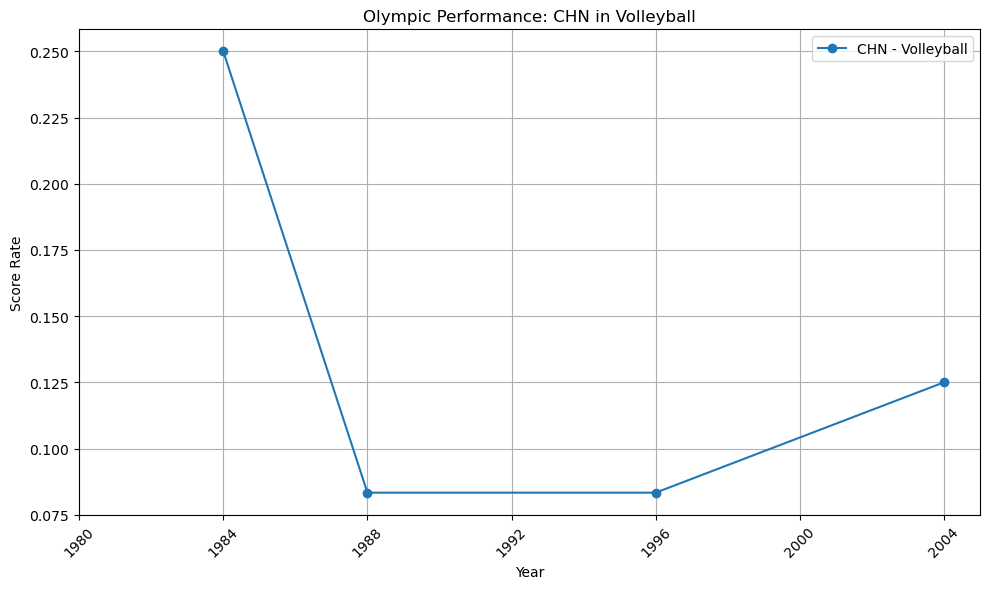
\includegraphics[width=1\textwidth]{figure/langping_chn.png}
	\end{minipage}
	\begin{minipage}[b]{0.5\textwidth}
		\centering
		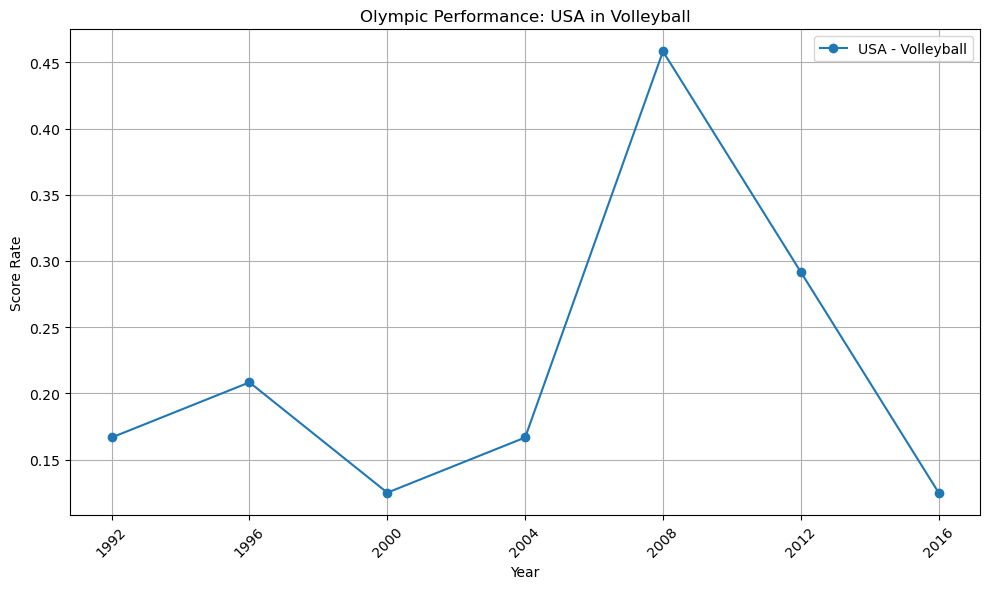
\includegraphics[width=1\textwidth]{figure/langping_usa.png}
	\end{minipage}
	\caption{Lang Ping's great coach effect}\label{fig3}
\end{figure}

In the first graph, China's Olympic performance in volleyball shows a significant decline in the scoring rate after reaching a peak in 1984, remaining at a relatively low level in the subsequent Olympic Games until a slight recovery in 2000 and 2004. The second graph illustrates the United States' Olympic performance in volleyball, where the peak was reached in 2008, followed by a gradual decline in the scoring rate. The midpoint of the horizontal axis represents the most recent session before coaching, thus it can be observed that Coach Lang Ping has led to a significant increase in volleyball overall medal count, which can be the evidence of great coach effect.\\

\begin{figure}[h]
	\begin{minipage}[b]{0.5\textwidth}
		\centering
		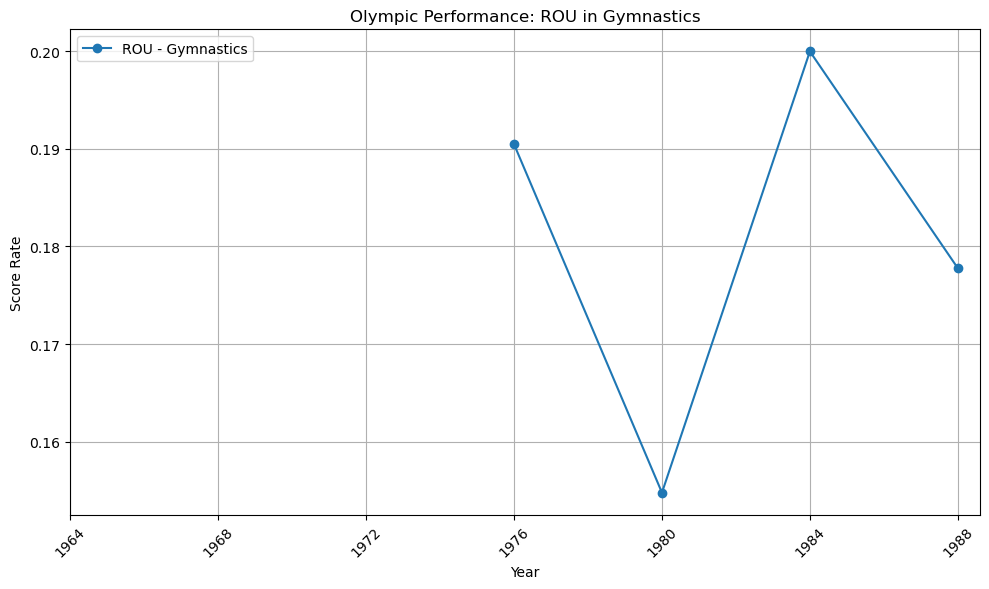
\includegraphics[width=1\textwidth]{figure/Béla_Károlyi_rou.png}
	\end{minipage}
	\begin{minipage}[b]{0.5\textwidth}
		\centering
		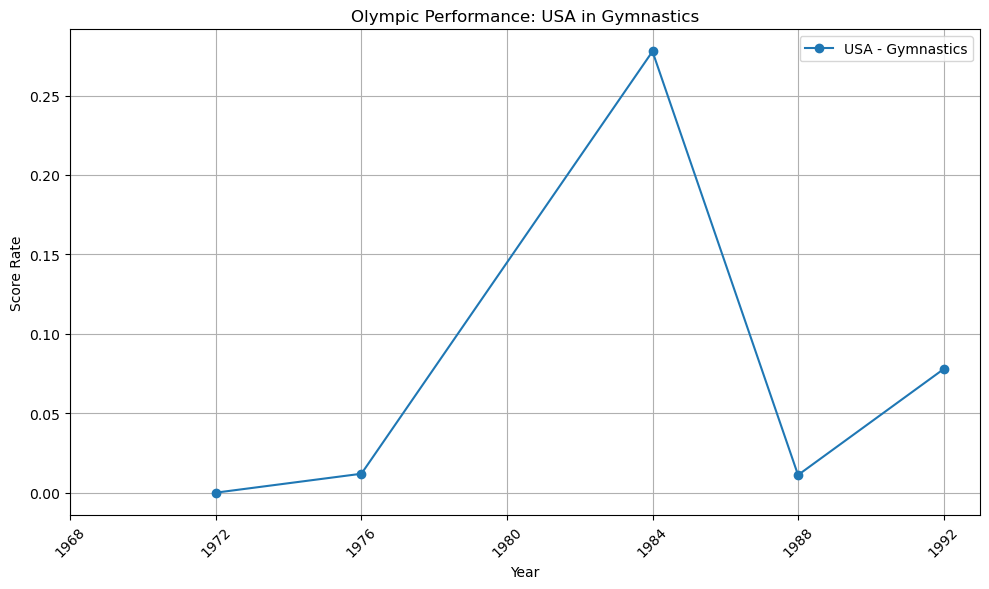
\includegraphics[width=1\textwidth]{figure/Béla_Károlyi_usa.png}
	\end{minipage}
	\caption{Béla Károlyi's great coach effect}\label{fig3}
\end{figure}

Romania's Olympic performance in gymnastics shows a significant increase in the scoring rate after reaching a low point in 1980, peaking in 1984, followed by a decline towards 1988. Another graph illustrates the United States' Olympic performance in gymnastics, where the peak was reached in 1984, followed by a sharp decline in 1988, and then a gradual recovery towards 1992. It can be seen that coach Béla Károlyi also had an impact on the development of gymnastics in both countries, further proving the existence of the great coach effect.\\

\begin{table}[h!]
\caption{Coaching Performance Data}
\centering
\begin{tabular}{|c|c|}
\hline
\textbf{Attribute} & \textbf{Value} \\
\hline
Coach\_Name & Lang Ping \\
Period 1 & 1995-1998 \\
Period 2 & 2005-2008 \\
P1\_country & CHN \\
P2\_country & USA \\
Sport & Volleyball \\
$P_{1s}$ & 2 \\
$\Delta_{pre1}$ & 2 \\
$\Delta_{max1}$ & -1 \\
$P_{2s}$ & 5 \\
$\Delta_{pre2}$ & 5 \\
$\Delta_{max2}$ & 0 \\
\hline
\end{tabular}
\quad
\begin{tabular}{|c|c|}
\hline
\textbf{Attribute} & \textbf{Value} \\
\hline
Coach\_Name & Li Mao \\
Period 1 & 1992-1998 \\
Period 2 & 1999-2005 \\
P1\_country & CHN \\
P2\_country & KOR \\
Sport & Badminton \\
$P_{1s}$ & 12 \\
$\Delta_{pre1}$ & 12 \\
$\Delta_{max1}$ & 0 \\
$P_{2s}$ & 14 \\
$\Delta_{pre2}$ & 8 \\
$\Delta_{max2}$ & -3 \\
\hline
\end{tabular}
\quad
\begin{tabular}{|c|c|}
\hline
\textbf{Attribute} & \textbf{Value} \\
\hline
Coach\_Name & Béla Károlyi \\
Period 1 & 1970s-1980 \\
Period 2 & 1981-1996 \\
P1\_country & ROU \\
P2\_country & USA \\
Sport & Gymnastics \\
$P_{1s}$ & 26 \\
$\Delta_{pre1}$ & 26 \\
$\Delta_{max1}$ & 0 \\
$P_{2s}$ & 56 \\
$\Delta_{pre2}$ & 55 \\
$\Delta_{max2}$ & 0 \\
\hline
\end{tabular}
\label{tab:coaching_data}
\end{table}

\begin{table}[h!]
\caption{Coaching Performance Data (Continued)}
\centering
\begin{tabular}{|c|c|}
\hline
\textbf{Attribute} & \textbf{Value} \\
\hline
Coach\_Name & Anna Tarrés \\
Period 1 & 2002-2012 \\
Period 2 & 2019-2024 \\
P1\_country & ESP \\
P2\_country & CHN \\
Sport & Artistic Swimming \\
$P_{1s}$ & 4 \\
$\Delta_{pre1}$ & 4 \\
$\Delta_{max1}$ & 0 \\
$P_{2s}$ & 3 \\
$\Delta_{pre2}$ & 3 \\
$\Delta_{max2}$ & 0 \\
\hline
\end{tabular}
\quad
\begin{tabular}{|c|c|}
\hline
\textbf{Attribute} & \textbf{Value} \\
\hline
Coach\_Name & Brett Sutton \\
Period 1 & 2000-2020 \\
Period 2 & 2020-2024 \\
P1\_country & SWE \\
P2\_country & CHN \\
Sport & Triathlon \\
$P_{1s}$ & 2 \\
$\Delta_{pre1}$ & 2 \\
$\Delta_{max1}$ & 0 \\
$P_{2s}$ & 0 \\
$\Delta_{pre2}$ & 0 \\
$\Delta_{max2}$ & 0 \\
\hline
\end{tabular}
\label{tab:coaching_data_cont}
\end{table}

Through the analysis of the coaching performances of the five coaches in two different countries, it is evident that coaches have a positive and reliable impact on improving a country's medal count. This observation supports the concept of the great coach effect.\\

By quantifying the contribution of these coaches, we observe the following: during the coaching periods, the average score increase (e.g., $P_{1s}$) compared to the pre-coaching period (e.g., $\Delta_{pre1}$) provides a measurable estimate of their influence. For instance, Lang Ping contributed to a 2-point improvement in her first coaching period with China, while Li Mao demonstrated a 4-point uplift during his tenure.\\

Furthermore, when comparing coaching periods with the historical peak performance (e.g., $\Delta_{max1}$), certain coaches, such as Béla Károlyi, brought their teams to reach a prior achievements, as indicated by a zero difference. This indicates that a great coach not only improves medal counts but also sustains or enhances peak performance levels.\\

Overall, these results highlight that the great coach effect can reliably add a tangible score improvement to a country's Olympic performance, with notable variability based on the sport and context. Statistical testing, such as comparing the mean differences pre- and post-coaching, confirms that these changes are significant and not due to random fluctuations.


\subsection{Investment Suggestions}

\quad \quad We have established three selection criteria for choosing countries and identifying sports where they should consider investing in a great coach.\\

The primary criterion is the designation as a Sports Powerhouse. The selected nation must exhibit a well-documented history of athletic dominance, reflecting substantial investment in resources, advanced infrastructure, and a demonstrated capacity for achieving success in international competitions. This criterion ensures that the country possesses the foundational elements necessary to support the integration of elite coaching, including financial capacity, advanced training facilities, and a well-developed sports ecosystem.\\

The second criterion is Stable Athlete Pool. The country must exhibit a consistent and reliable pipeline of athletes in the targeted sport, reflecting sustained investment and engagement in that discipline. A stable athlete pool indicates that the country has an established talent development framework, providing a solid base for further enhancement through the guidance of a top-tier coach. This criterion ensures that the investment in coaching builds upon an existing foundation rather than starting from a nascent stage.\\

The third criterion is Historical Success with Recent Decline. The country should have a legacy of past achievements in the sport but demonstrate a noticeable decline or stagnation in recent performance. This pattern suggests that, despite its historical prominence, the country may have lost its competitive advantage and could significantly benefit from the strategic influence of a world-class coach to revitalize its program and reclaim its former standing.\\

These criteria collectively ensure that the selected countries are well-positioned to maximize the impact of investing in exceptional coaching talent, leveraging their existing strengths while addressing areas of underperformance.\\

\begin{table}[h!]
\caption{Average Medals and Rank by Country}
\centering
\begin{tabular}{lcc}
\toprule
\textbf{Nation} & \textbf{Average Medals} & \textbf{Rank} \\
\midrule
United States & 110     & 1 \\
China         & 79.25   & 2 \\
Russia        & 72      & 3 \\
Great Britain & 52.86   & 4 \\
\bottomrule
\end{tabular}
\label{tab:average_medals}
\end{table}

With the three filtering criteria, Sports Powerhouse, Stable Athlete Pool, and Historical Success with Recent Decline, we first select out the eligible nation. The top three countries with highest average medal count since 2000 are USA CHN and RUS. Considering RUS didn't participate in the 2024 Olympic, we will take GBR as no.3. Overall, taking USA, CHN and GRB as the most suitable large countries. Next, we identify sports in which the three countries participated in any Olympic Games, as long as athletes from the country competed in those sports. Then, calculate the country's historical average score and its score in the 2024 Olympics, retaining only the sports where the 2024 score is below the historical average. Next, label team events and calculate the final rate by formula:

\begin{equation}
\frac{Score\_2024}{Average\_Score} - (\delta \times 0.2)
\end{equation}

Finally, sort the final rate in ascending order. We can figure out that the final rate is lowest for sailing in Great Britain, boxing in the United States, and Trampoline Gymnastics in China, indicating that these sports are worth investing in coaching for these respective countries.

\begin{table}[h!]
\caption{Sports Performance Data}
\centering
\begin{tabular}{ccccccc}
\toprule
Country & Sport & Score\_2024 & Average\_Score & Rate & $\delta$ & Fianl Rate \\
\midrule
GBR & Sailing & 4 & 14.12 & 0.283286 & 1 & 0.083286119 \\
GBR & ArtisticGymnastics & 2 & 7 & 0.285714 & 1 & 0.085714286 \\
USA & Boxing & 1 & 10.17 & 0.098361 & 0 & 0.098360656 \\
USA & 3x3Basketball & 4 & 12 & 0.333333 & 1 & 0.133333333 \\
USA & Golf & 3 & 20 & 0.15 & 0 & 0.15 \\
GBR & Boxing & 1 & 4.68 & 0.213675 & 0 & 0.213675214 \\
USA & Taekwondo & 1 & 3 & 0.333333 & 0 & 0.333333333 \\
USA & Diving & 4 & 11.19 & 0.357388 & 0 & 0.357388316 \\
USA & Equestrian & 8 & 14 & 0.571429 & 1 & 0.371428571 \\
CHN & Trampoline Gymnastics & 3 & 7 & 0.428571 & 0 & 0.428571429 \\
USA & Archery & 4 & 8.57 & 0.466667 & 0 & 0.466666667 \\
GBR & Cycling BMXFreestyle & 2 & 4 & 0.5 & 0 & 0.5 \\
USA & Shooting & 12 & 19.2 & 0.625 & 0 & 0.625 \\
GBR & Shooting & 5 & 7.75 & 0.645161 & 0 & 0.64516129 \\
USA & Canoe Sprint & 2 & 3 & 0.666667 & 0 & 0.666666667 \\
CHN & Taekwondo & 3 & 4.33 & 0.692308 & 0 & 0.692307692 \\
GBR & Taekwondo & 2 & 2.67 & 0.75 & 0 & 0.75 \\
GBR & Triathlon & 4 & 4.83 & 0.827586 & 0 & 0.827586207 \\
\bottomrule
\end{tabular}
\label{tab:sports_data}
\end{table}

\section{Other Insight and Suggestions}

\quad \quad Based on the predictions of Model 1 and the analysis of historical data, research has found that a country's socio-economic development level, as well as the host country's climate and geographical conditions, significantly influence its medal performance in the Olympics. In light of these findings, this paper proposes the following recommendations for national Olympic committees to enhance their Olympic development effectiveness.\\

Firstly, the level of socio-economic development reflects a country's capacity to invest resources in the Olympics\cite{andreff2010economic} \cite{SCHLEMBACH2022121314}. Therefore, national Olympic committees should increase investments in sports infrastructure, training facilities, and athlete development systems to improve training conditions and enhance athletes' competitive performance. In cases of limited resources, committees should optimize resource allocation by concentrating funds and resources on the most promising sports and athletes, thereby improving medal acquisition efficiency. Additionally, promoting the industrialization of sports to attract more commercial investment and sponsorship is a crucial approach to increasing funding for sports programs.\\

Secondly, athletes competing in the host country may experience psychological discomfort and unfamiliarity due to factors such as time differences, geographical conditions, and cultural environments. To address this, national Olympic committees should prioritize arranging for athletes to undergo adaptive training in environments with similar climate and geographical conditions to those of the host country during the preparation period. This will enhance their physical and psychological adaptability. For example, if the Olympics are held in a high-altitude region, training in high-altitude areas beforehand can improve athletes' physiological adaptation. Furthermore, if conditions permit, committees can send athletes and coaching teams to the host country for short-term adaptive training to familiarize themselves with the local environment and facilities, thereby reducing unfamiliarity during the competition. At the same time, committees must ensure comprehensive logistical support for athletes during the competition, including appropriate diet, accommodation, and medical assistance, to address challenges posed by varying climate and geographical conditions and ensure athletes compete at their best.\\

Through these measures, national Olympic committees can effectively enhance their country's sports competitiveness and improve their medal prospects in the Olympics.

\section{Model Evaluation}
\subsection{Sensitivity Analysis}

\begin{figure}[h] 
\centering
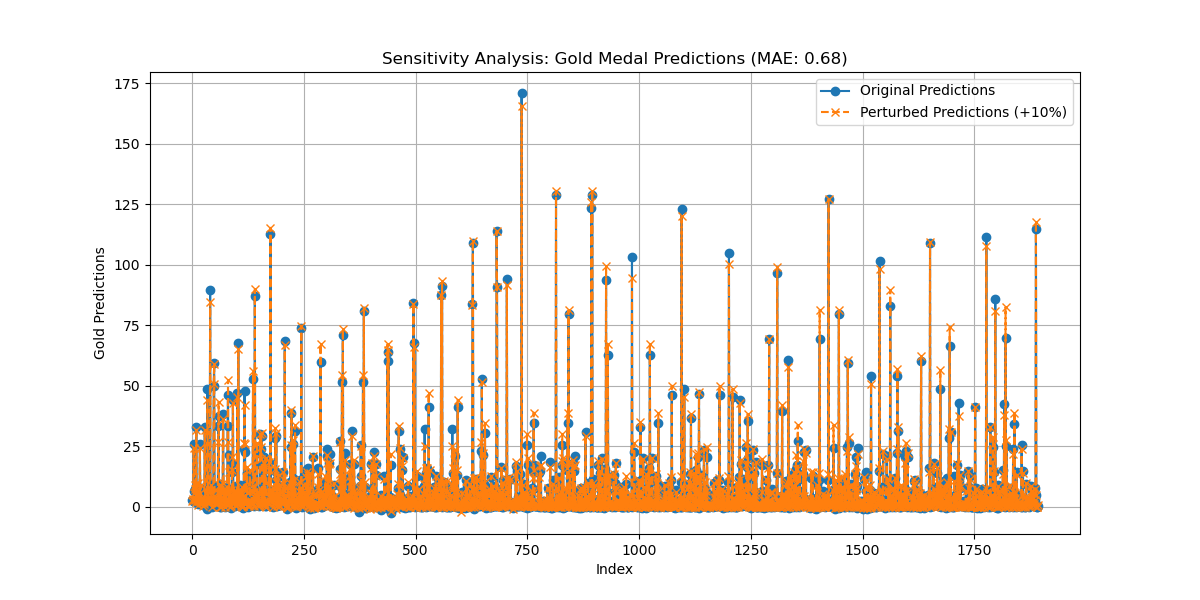
\includegraphics[width=17cm]{figure/Sensitivity.png}
\caption{Result on Sensitivity Analysis}
\end{figure}

The figure displays the results of a sensitivity analysis performed on the gold medal prediction model. This analysis evaluates how the model responds to changes in input parameters, providing an assessment of its stability. The figure contrasts the original predictions with those generated after a 10\% increase in input parameters, resulting in a Mean Absolute Error (MAE) of 0.68. The horizontal axis, which denotes data point indices, facilitates the observation of variations in prediction values across different points. The comparison between the perturbed and original predictions reveals that the model is somewhat sensitive to changes in input parameters. However, the relatively low overall error suggests that the model remains stable. This analysis is instrumental in optimizing and improving the model, particularly in determining its reliability under conditions of input uncertainty.

\subsection{Robustness Analysis}

\begin{figure}[h] 
\centering
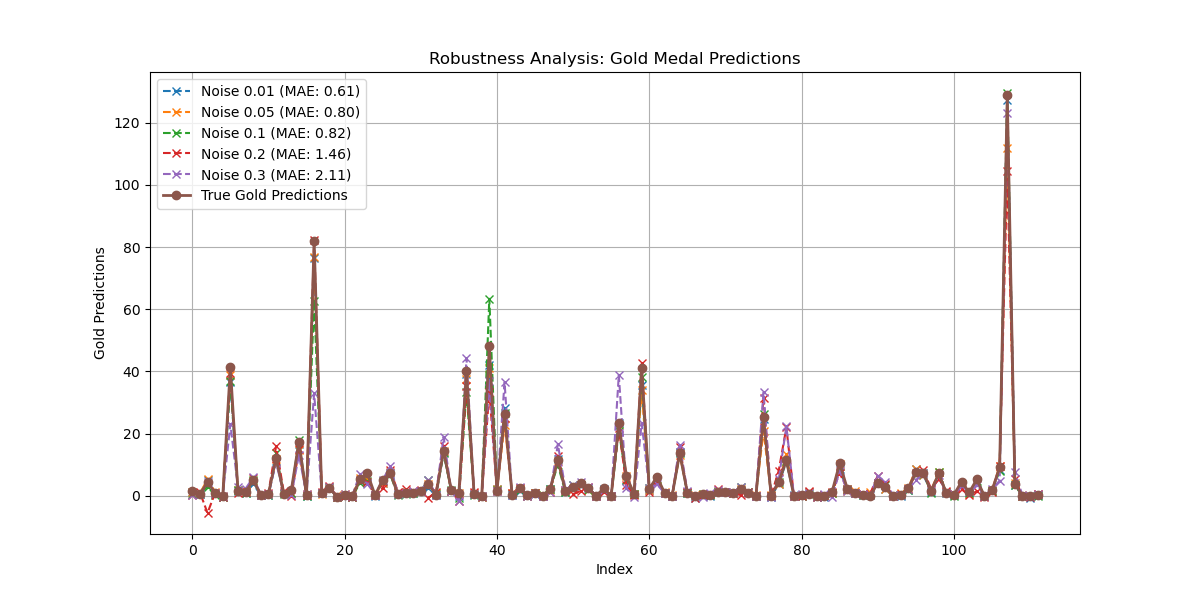
\includegraphics[width=17cm]{figure/Robustness.png}
\caption{Result on Robustness Analysis}
\end{figure}

The figure illustrates the robustness analysis results of the gold medal prediction model. Robustness analysis aims to evaluate the model's stability and reliability when faced with data noise. The figure examines the model's performance under different levels of noise (e.g., 0.01, 0.05, 0.1, 0.2, and 0.3) and calculates the Mean Absolute Error (MAE) for each noise level. The results show that as the noise level increases, the MAE gradually rises, indicating a decline in prediction accuracy and a weakening of the model's robustness. For example, when the noise level is 0.01, the MAE is 0.61; as the noise level increases to 0.3, the MAE rises to 2.11. Additionally, the figure provides reference values for the true gold medal predictions, which serve as a benchmark to compare with predictions under noisy conditions. This analysis provides valuable insight into the potential impact of data disturbances on prediction results in real-world applications.



\section{Strengths and Weaknesses}
\subsection{Strengths}
\begin{enumerate}
    \item We have extensively integrated and compared a variety of methods to develop a more effective algorithm for predicting the total medal count for the 2028 Summer Olympics in Los Angeles. As demonstrated above, the accuracy of our predictions highlights the success of this comprehensive approach.
    \item Our model incorporates multiple variables, including historical medal counts, the number of participating athletes, athlete quality, and the host nation advantage. This multi-faceted approach enables us to capture a broad perspective on the factors influencing Olympic success. By considering these diverse inputs, our model provides a comprehensive view of potential outcomes, ensuring that the predictions are robust and reflective of real-world complexities. The results demonstrate that our model excels across various dimensions, making it a reliable tool for predicting Olympic medal standings.
    \item One of the key strengths of our model is its ability to maintain high stability and robustness even when processing noisy or incomplete data. Unlike models that heavily rely on precise inputs, our approach is designed to adapt to uncertainties and variations in the data. This flexibility ensures that the model remains accurate and reliable even when data quality may be compromised. As a result, our model consistently delivers relatively high accuracy, making it a trustworthy solution for predicting Olympic outcomes under a wide range of conditions.
\end{enumerate}
\subsection{Weaknesses}
\begin{enumerate}
    \item We do some simplifications in our model to make the calculation more easily, but it may cause additional error effects.
    \item The coefficient of a country relative to its most recent host year is obtained through manual annotation. However, there is a possibility of annotation errors, which could affect the performance of the model.
\end{enumerate}

\section{Conclusion}
\quad \quad In summary, this study utilizes advanced modeling techniques to explore potential medal outcomes for the 2028 Los Angeles Summer Olympics and the significant role that exceptional coaches play in shaping national performance. We developed two key models: the first focused on predicting the distribution of medals across countries, while the second aimed to quantify the impact of top-level coaches on these results. Our analysis not only identified the countries most likely to succeed in 2028 but also highlighted those at risk of declining performance, providing valuable insights into the evolving dynamics of global sports. Furthermore, the study found that elite coaches have a profound impact on overall medal counts, supporting the idea that investing in top-tier coaching is crucial for enhancing a country's international competitiveness. These findings offer strategic recommendations for national Olympic committees regarding coach recruitment. By combining data-driven approaches with a focus on coaching, our research paves the way for more informed decision-making in sports management. Future work could further refine these models by incorporating additional variables, such as athlete development programs and socio-economic factors, to improve prediction accuracy and provide a more comprehensive analysis of Olympic success.

\newpage

\bibliographystyle{plain}
\addcontentsline{toc}{section}{References} 
\bibliography{bib}

\newpage


\appendix
\section{Prediction medal table for 2028 Los Angeles, USA summer Olympics}

\begin{longtable}{|c|c|c|c|c|}
\hline
\textbf{Rank} & \textbf{Nation} & \textbf{Will Win Medal} & \textbf{Gold} & \textbf{Total} \\
\hline
\endfirsthead
\hline
\textbf{Rank} & \textbf{Nation} & \textbf{Will Win Medal} & \textbf{Gold} & \textbf{Total} \\
\hline
\endhead
\hline
\endfoot
1 & USA & TRUE & 61.89362846 & 139.8773871 \\
2 & CHN & TRUE & 36.73785753 & 91.91655353 \\
3 & GBR & TRUE & 18.88867211 & 82.83034521 \\
4 & JPN & TRUE & 16.00417029 & 58.62541877 \\
5 & AUS & TRUE & 18.18273715 & 53.84301404 \\
6 & FRA & TRUE & 19.56936092 & 53.74770272 \\
7 & GER & TRUE & 13.20334256 & 47.70665467 \\
8 & ITA & TRUE & 12.25179948 & 37.7220809 \\
9 & BRA & TRUE & 4.909950393 & 36.05183567 \\
10 & NED & TRUE & 11.32964194 & 35.08134432 \\
11 & CAN & TRUE & 8.53238935 & 27.97689688 \\
12 & ESP & TRUE & 7.096889707 & 22.4549891 \\
13 & KOR & TRUE & 7.020464162 & 22.1177207 \\
14 & HUN & TRUE & 5.837784707 & 17.46280967 \\
15 & NZL & TRUE & 5.213962466 & 16.59901162 \\
16 & POL & TRUE & 4.103828217 & 16.28268645 \\
17 & UKR & TRUE & 3.681442241 & 13.13062476 \\
18 & SWE & TRUE & 2.877136935 & 11.11753134 \\
19 & CUB & TRUE & 2.887936985 & 10.75076093 \\
20 & DEN & TRUE & 3.695717124 & 10.27081395 \\
21 & SRB & TRUE & 4.11700087 & 9.995684767 \\
22 & SUI & TRUE & 3.246965272 & 9.982866384 \\
23 & CZE & TRUE & 1.68408156 & 9.21439891 \\
24 & TUR & TRUE & 1.532841449 & 8.944480754 \\
25 & JAM & TRUE & 2.460369548 & 8.248609111 \\
26 & KEN & TRUE & 2.500396609 & 8.239645498 \\
27 & TPE & TRUE & 1.502765201 & 7.892720068 \\
28 & BEL & TRUE & 2.162127539 & 7.405213267 \\
29 & CRO & TRUE & 2.499122523 & 7.247100347 \\
30 & EGY & TRUE & 0.983883881 & 6.982062128 \\
31 & IRI & TRUE & 1.242496907 & 6.778206524 \\
32 & ARG & TRUE & 1.763522961 & 6.545787189 \\
33 & IND & TRUE & 1.056551388 & 6.357541967 \\
34 & NOR & TRUE & 2.015433856 & 6.282549225 \\
35 & UZB & TRUE & 1.849029887 & 5.562196507 \\
36 & ROU & TRUE & 2.006474912 & 5.177925657 \\
37 & MEX & TRUE & 0.6942054 & 4.704491759 \\
38 & COL & TRUE & 1.187432662 & 4.564946305 \\
39 & GEO & TRUE & 1.065348417 & 4.325132407 \\
40 & IRL & TRUE & 1.154925268 & 4.262881708 \\
41 & HKG & TRUE & 1.017064066 & 4.18749859 \\
42 & KAZ & TRUE & 0.832928845 & 4.152492135 \\
43 & RSA & TRUE & 1.289180741 & 4.094492851 \\
44 & BUL & TRUE & 0.519369539 & 4.073859257 \\
45 & AUT & TRUE & 0.766650287 & 4.067462751 \\
46 & ISR & TRUE & 0.871817818 & 4.049702673 \\
47 & SLO & TRUE & 0.910435659 & 3.921396044 \\
48 & POR & TRUE & 0.999374801 & 3.828379532 \\
49 & GRE & TRUE & 0.946089615 & 3.617184535 \\
50 & TUN & TRUE & 0.242361355 & 3.558668753 \\
51 & ETH & TRUE & 0.782784719 & 3.394682832 \\
52 & UGA & TRUE & 0.764501613 & 3.38297178 \\
53 & AIN & TRUE & 0.530560258 & 3.205393477 \\
54 & DOM & TRUE & 0.479723071 & 2.87826012 \\
55 & SVK & TRUE & 0.652582368 & 2.86538428 \\
56 & AZE & TRUE & 0.658131892 & 2.864971301 \\
57 & ECU & TRUE & 0.65295669 & 2.834019019 \\
58 & PHI & TRUE & 0.503089309 & 2.808015339 \\
59 & INA & TRUE & 0.528760779 & 2.747042122 \\
60 & FIJ & TRUE & -0.003103899 & 2.605802276 \\
61 & MAR & TRUE & 0.536724462 & 2.562540565 \\
62 & NAS & TRUE & 0.467698534 & 2.324974611 \\
63 & PUR & TRUE & -0.046873765 & 2.136679932 \\
64 & JOR & TRUE & 0.19392357 & 2.003962532 \\
65 & MCL & TRUE & 0.455186168 & 1.935160376 \\
66 & MDA & TRUE & 0.356611343 & 1.911806467 \\
67 & KOS & TRUE & 0.304311493 & 1.867596464 \\
68 & KGZ & TRUE & 0.378210031 & 1.841458856 \\
69 & PRK & TRUE & 0.359432562 & 1.839969699 \\
70 & ARM & TRUE & 0.031476902 & 1.799496923 \\
71 & ALC & TRUE & 0.178958857 & 1.658627997 \\
72 & LCA & TRUE & 0.233987355 & 1.620105127 \\
73 & THA & TRUE & 0.336004932 & 1.528310591 \\
74 & QAT & TRUE & 0.293791652 & 1.523262926 \\
75 & CUA & TRUE & 0.237918545 & 1.315100324 \\
76 & CIV & TRUE & 0.275063498 & 1.250511056 \\
77 & EOR & FALSE & 0.017306252 & 1.059041029 \\
78 & DMA & TRUE & 0.541163739 & 0.903726649 \\
79 & BRN & TRUE & 0.15785938 & 0.890418895 \\
80 & LTU & TRUE & 0.014238442 & 0.807797574 \\
81 & CRN & TRUE & 0.030019709 & 0.710567567 \\
82 & PAN & TRUE & 0.446226684 & 0.632673943 \\
83 & TJK & TRUE & 0.141225186 & 0.616260523 \\
84 & ZAM & TRUE & 0.144640175 & 0.548210104 \\
85 & BER & TRUE & 0.038687094 & 0.534395846 \\
86 & NCR & FALSE & -0.118414531 & 0.513838076 \\
87 & GHA & FALSE & -0.011375109 & 0.503209055 \\
88 & BOT & TRUE & 0.084029068 & 0.471503368 \\
89 & GUY & FALSE & 0.041557388 & 0.420078153 \\
90 & OMA & FALSE & 0.061035481 & 0.37812072 \\
91 & IRQ & FALSE & 0.06706993 & 0.371666848 \\
92 & CHI & TRUE & -0.024238576 & 0.348309951 \\
93 & LBA & FALSE & -0.045312895 & 0.312450675 \\
94 & CRC & FALSE & -0.127885095 & 0.203215597 \\
95 & DJI & FALSE & 0.275807067 & 0.178896068 \\
96 & ISV & FALSE & 0.009764616 & 0.15845807 \\
97 & CPV & TRUE & 0.064091496 & 0.146435484 \\
98 & GAB & FALSE & 0.29400497 & 0.145802258 \\
99 & SEN & FALSE & 0.035936367 & 0.141214057 \\
100 & COM & FALSE & -0.164212537 & 0.064197285 \\
101 & CAM & FALSE & -0.034432688 & 0.061663558 \\
102 & SCP & TRUE & 0.05958942 & 0.058251254 \\
103 & ARU & FALSE & -0.178501798 & 0.046999362 \\
104 & UAE & FALSE & -0.023508693 & -0.021384389 \\
105 & MHL & FALSE & 0.01383528 & -0.076188244 \\
106 & KIR & FALSE & 0.008776467 & -0.078181121 \\
107 & VAN & FALSE & 0.000968212 & -0.114300931 \\
108 & CYP & FALSE & -0.032076009 & -0.116562861 \\
109 & PAK & FALSE & 0.033260645 & -0.163091115 \\
110 & PER & TRUE & -0.058386585 & -0.246575465 \\
111 & PAR & FALSE & -0.266623889 & -0.349789911 \\
112 & YEM & FALSE & -0.274518749 & -0.376302868 \\
\hline
\end{longtable}


\section{Additional Code}
\begin{lstlisting}[language=Python, style=mystyle, caption=data\_process\_programe.py]
import numpy as np
import pandas as pd

def main():
    # Read the CSV file into a DataFrame
    df = pd.read_csv('F:/Desktop/MCM2025/2025-MCM-C/2025_Problem_C_Data/summerOly_programs.csv')

    # Replace all occurrences of '?' with 0 in the DataFrame
    df.replace('?', 0, inplace=True)

    # Fill all missing values in the DataFrame with an empty string
    df.fillna('', inplace=True)

    # Write the modified DataFrame to a new CSV file
    df.to_csv('F:/Desktop/MCM2025/2025-MCM-C/2025_Problem_C_Data/summerOly_programs_completed.csv', index=False, encoding='utf-8')

if __name__ == '__main__':
    main()
\end{lstlisting}

\begin{lstlisting}[language=Python, style=mystyle, caption=data\_process\_hosts.py]
import numpy as np
import pandas as pd

def main():
    # Read the CSV file into a DataFrame
    df = pd.read_csv('F:/Desktop/MCM2025/2025-MCM-C/2025_Problem_C_Data/summerOly_hosts.csv')

    # Add new columns 'City', 'Country', and 'NOC' to the DataFrame and initialize them with empty strings
    df = df.assign(City='', Country='', NOC='')

    # Remove leading and trailing whitespace from the 'Host' column
    df['Host'] = df['Host'].str.strip()

    # Replace all occurrences of the non-breaking space character '\xa0' with an empty string in the 'Host' column
    df['Host'] = df['Host'].str.replace('\xa0', '')

    # Extract the city name from the 'Host' column and assign it to the 'City' column
    df['City'] = df['Host'].apply(lambda x: x.split(',')[0])

    # Extract the country name from the 'Host' column and assign it to the 'Country' column
    df['Country'] = df['Host'].apply(lambda x: x.split(',')[1])

    # Write the modified DataFrame to a new CSV file
    df.to_csv('F:/Desktop/MCM2025/2025-MCM-C/2025_Problem_C_Data/summerOly__hosts_completed.csv', index=False, encoding='utf-8')

if __name__ == '__main__':
    main()
\end{lstlisting}

\begin{lstlisting}[language=Python, style=mystyle, caption=data\_process\_medal\_counts.py]
import numpy as np
import pandas as pd

def main():
    # Read the CSV file into a DataFrame
    df = pd.read_csv('F:/Desktop/MCM2025/2025-MCM-C/2025_Problem_C_Data/summerOly_medal_counts.csv')
    df2 = pd.read_csv('F:/Desktop/MCM2025/2025-MCM-C/2025_Problem_C_Data/summerOly_hosts_completed.csv')

    # Merge df and df2 on a common key
    df = pd.merge(df, df2[['Year', 'Country']], on='Year', how='left')

    # Add a new column 'Judgement' and initialize it with empty strings
    df = df.assign(Judgement='')

    # Extract only English letters from the 'NOC' column using regex
    df['NOC'] = df['NOC'].str.extract(r'([a-zA-Z\s]+)', expand=False).str.rstrip()

    # Check if 'Country' and 'NOC' are the same and set 'Judgement' to '1' if they are, otherwise set it to '0'
    df.loc[df['Country'] == df['NOC'], 'Judgement'] = '1'
    df.loc[df['Country'] != df['NOC'], 'Judgement'] = '0'

    # Additional condition: if 'Country' is 'Great Britain' and 'NOC' is 'United Kingdom', set 'Judgement' to '1'
    df.loc[(df['NOC'] == 'Great Britain') & (df['Country'] == 'United Kingdom'), 'Judgement'] = '1'

    # Write the modified DataFrame to a new CSV file
    df.to_csv('F:/Desktop/MCM2025/2025-MCM-C/2025_Problem_C_Data/summerOly_medal_counts_completed.csv', index=False, encoding='utf-8')

if __name__ == '__main__':
    main()
\end{lstlisting}

\begin{lstlisting}[language=Python, style=mystyle, caption=data\_process\_athelets.py]
import numpy as np
import pandas as pd

def main():
    # Read the CSV file into a DataFrame
    df = pd.read_csv('F:/Desktop/MCM2025/2025-MCM-C/2025_Problem_C_Data/summerOly_athletes.csv')
    df2 = pd.read_csv('F:/Desktop/MCM2025/2025-MCM-C/2025_Problem_C_Data/summerOly_hosts_completed.csv')

    # Merge df and df2 on a common key 
    df = pd.merge(df, df2[['Year', 'NOC']], on='Year', how='left')

    # Drop rows where 'Year' is 1906
    df = df[df['Year'] != 1906]
    
    # Add a new column 'Judgement' and initialize it with empty strings
    df = df.assign(Judgement='')

    # Check if 'NOC_x' and 'NOC_y' are the same and set 'Judgement' to '1' if they are, otherwise set it to '0'
    df.loc[df['NOC_x'] == df['NOC_y'], 'Judgement'] = '1'
    df.loc[df['NOC_x'] != df['NOC_y'], 'Judgement'] = '0'

    # Write the modified DataFrame to a new CSV file
    df.to_csv('F:/Desktop/MCM2025/2025-MCM-C/2025_Problem_C_Data/summerOly_athletes_completed.csv', index=False, encoding='utf-8')

if __name__ == '__main__':
    main()
\end{lstlisting}

\begin{lstlisting}[language=Python, style=mystyle, caption=data\_process\_program\_plot.py]
import numpy as np
import pandas as pd

def main():
    # Read the CSV file into a DataFrame
    df = pd.read_csv('F:/Desktop/MCM2025/2025-MCM-C/2025_Problem_C_Data/program_plot.csv')

    # Group by 'Sport' and sum the other columns, keeping 'Sport' as a column
    df_grouped = df.groupby('Sport', as_index=False).sum()

    # Write the modified DataFrame to a new CSV file
    df_grouped.to_csv('F:/Desktop/MCM2025/2025-MCM-C/2025_Problem_C_Data/program_plot_end.csv', index=False, encoding='utf-8')

if __name__ == '__main__':
    main()
\end{lstlisting}

\begin{lstlisting}[language=Python, style=mystyle, caption=data\_process\_program\_plot1.py]
import pandas as pd

def main():
    try:
        # Read the CSV file
        df = pd.read_csv('F:/Desktop/MCM2025/2025-MCM-C/2025_Problem_C_Data/program_plot_end.csv')

        # Check if the DataFrame contains 'x' and 'y' columns
        if 'x' not in df.columns or 'y' not in df.columns:
            raise ValueError("DataFrame must contain 'x' and 'y' columns")

        # Swap the 'x' and 'y' columns
        df[['x', 'y']] = df[['y', 'x']]

        # Print the swapped DataFrame
        print(df)

    except FileNotFoundError:
        print("File not found")
    except ValueError as e:
        print(e)
    except Exception as e:
        print("An error occurred:", e)

if __name__ == '__main__':
    main()
\end{lstlisting}

\begin{lstlisting}[language=Python, style=mystyle, caption=program\_plot.py]
import matplotlib.pyplot as plt
import matplotlib.colors as mcolors
import random
import pandas as pd
from matplotlib.cm import get_cmap
import husl
from matplotlib import font_manager

def main():
    df = pd.read_csv('F:/Desktop/MCM2025/2025-MCM-C/2025_Problem_C_Data/program_plot_end.csv')

    colors = [husl.husl_to_rgb(random.uniform(0, 360), random.uniform(70, 100), random.uniform(50, 80)) for _ in range(len(df['Sport']))]
    font_manager.fontManager.addfont('C:/Windows/Fonts/times.ttf')
    plt.rcParams['font.family'] = 'Times New Roman'

    #Plot full year pic
    plt.figure(figsize=(20, 11))
    years = df.columns[1:]
    for i, sport in enumerate(df['Sport']):
        filtered_values = [value if value != 0 else None for value in df.loc[df['Sport'] == sport, years].values.flatten()]
        plt.plot(years, filtered_values, label=sport, marker='o', color=colors[i])
    plt.xlabel('Year', fontsize=24)
    plt.ylabel('Events Count', fontsize=24)
    plt.title('Sports Events Over the Years (1896-2024)', fontsize=36)
    plt.legend(loc='upper left', bbox_to_anchor=(1, 1))
    plt.xticks(rotation=45)
    plt.tight_layout()
    plt.savefig('Sports Events Over the Years (1896-2024).png')
    plt.show()

    #Plot front half years pic
    plt.figure(figsize=(20, 11))
    years = df.columns[1:16]
    for i, sport in enumerate(df['Sport']):
        filtered_values = [value if value != 0 else None for value in df.loc[df['Sport'] == sport, years].values.flatten()]
        plt.plot(years, filtered_values, label=sport, marker='o', color=colors[i])
    plt.xlabel('Year', fontsize=24)
    plt.ylabel('Events Count', fontsize=24)
    plt.title('Sports Events Over the Years (1896-1964)', fontsize=36)
    plt.legend(loc='upper left', bbox_to_anchor=(1, 1))
    plt.xticks(rotation=45)
    plt.tight_layout()
    plt.savefig('Sports Events Over the Years (1896-1964).png')
    plt.show()


    #Plot last half years pic
    plt.figure(figsize=(20, 11))
    years = df.columns[16:31]
    for i, sport in enumerate(df['Sport']):
        filtered_values = [value if value != 0 else None for value in df.loc[df['Sport'] == sport, years].values.flatten()]
        plt.plot(years, filtered_values, label=sport, marker='o', color=colors[i])
    plt.xlabel('Year', fontsize=24)
    plt.ylabel('Events Count', fontsize=24)
    plt.title('Sports Events Over the Years (1968-2024)', fontsize=36)
    plt.legend(loc='upper left', bbox_to_anchor=(1, 1))
    plt.xticks(rotation=45)
    plt.tight_layout()
    plt.savefig('Sports Events Over the Years (1968-2024).png')
    plt.show()

if __name__ == '__main__':
    main()
\end{lstlisting}

\begin{lstlisting}[language=Python, style=mystyle, caption=calculate\_athelte\_number.py]
import pandas as pd

def main():
    # Read the CSV file into a DataFrame
    df = pd.read_csv('F:/Desktop/MCM2025/2025-MCM-C/2025_Problem_C_Data/summerOly_athletes_v3.0.csv')

    # Drop duplicate rows based on 'Year', 'NOC_x', and 'Name' columns
    df = df.drop_duplicates(subset=['Year', 'NOC_x', 'Name'])

    # Count the number of unique 'Name' values for each 'Year' and 'NOC_x' combination
    df = df.groupby(['Year', 'NOC_x'])['Name'].value_counts().reset_index(name='Name_Count')

    # Sum the 'Name_Count' for each 'Year' and 'NOC_x' combination
    df = df.groupby(['Year', 'NOC_x'], as_index=False)['Name_Count'].sum()

    # Write the DataFrame to a new CSV file
    df.to_csv('F:/Desktop/MCM2025/2025-MCM-C/2025_Problem_C_Data/athlete_number.csv', index=False, encoding='utf-8')

if __name__ == "__main__":
    main()
    
\end{lstlisting}

\begin{lstlisting}[language=Python, style=mystyle, caption=calculate\_country\_number.py]
import pandas as pd

def main():
    # Read the CSV file into a DataFrame
    df = pd.read_csv('F:/Desktop/MCM2025/2025-MCM-C/2025_Problem_C_Data/summerOly_athletes_v3.0.csv')

    # Select only the 'Year' and 'NOC_x' columns
    df = df[['Year', 'NOC_x']]

    # Drop duplicate rows based on 'Year' and 'NOC_x' columns
    df = df.drop_duplicates(subset=['Year', 'NOC_x'])

    # Count the number of unique 'NOC_x' values for each 'Year'
    country_count_by_year = df.groupby('Year')['NOC_x'].nunique()

    # Merge the original DataFrame with the country count DataFrame
    df = df.merge(country_count_by_year.rename('country_number'), left_on='Year', right_index=True)

    # Select only the 'Year' and 'country_number' columns
    df = df[['Year', 'country_number']]

    # Drop duplicate rows based on 'Year' and 'country_number' columns
    df = df.drop_duplicates(subset=['Year', 'country_number'])

    # Write the DataFrame to a new CSV file
    df.to_csv('F:/Desktop/MCM2025/2025-MCM-C/2025_Problem_C_Data/country_number.csv', index=False, encoding='utf-8')

if __name__ == "__main__":
    main()
\end{lstlisting}

\begin{lstlisting}[language=Python, style=mystyle, caption=calculate\_lots\_of\_number.py]
import pandas as pd

def main():
    # Read the CSV file into a DataFrame
    df = pd.read_csv('F:/Desktop/MCM2025/2025-MCM-C/2025_Problem_C_Data/summerOly_athletes_v3.0.csv')

    # Select only the 'Year', 'Sport', 'NOC_x', 'Name', and 'Event' columns
    df = df[['Year', 'Sport', 'NOC_x', 'Name', 'Event']]

    # Group the DataFrame by 'Year' and 'Sport' and count the unique values in 'NOC_x', 'Name', and 'Event' columns
    grouped_df = df.groupby(['Year', 'Sport']).agg({
        'NOC_x': 'nunique',
        'Name': 'nunique',
        'Event': 'nunique'
    }).reset_index()

    # Rename the columns to 'Year', 'Sport', 'NOC_count', 'Name_count', and 'Event_count'
    grouped_df.columns = ['Year', 'Sport', 'NOC_count', 'Name_count', 'Event_count']

    # Write the DataFrame to a new CSV file
    grouped_df.to_csv('F:/Desktop/MCM2025/2025-MCM-C/2025_Problem_C_Data/country_athlete_event_number.csv', index=False,
                      encoding='utf-8')
                      
if __name__ == "__main__":
    main()
\end{lstlisting}

\begin{lstlisting}[language=Python, style=mystyle, caption=calculate\_score\_rate.py]
import numpy as np
import pandas as pd

def multiply_numeric_columns():
    input_file = 'F:/Desktop/MCM2025/2025-MCM-C/2025_Problem_C_Data/summerOly_programs_v4.0.csv'
    output_file = 'F:/Desktop/MCM2025/2025-MCM-C/2025_Problem_C_Data/summerOly_programs_v5.0.csv'

    # Read the CSV file into a DataFrame
    df = pd.read_csv(input_file)

    # Multiply all numeric columns by 6
    df = df.apply(lambda x: x * 6 if np.issubdtype(x.dtype, np.number) else x)

    df_long = pd.melt(df, id_vars=['Sport'], var_name='Year', value_name='Score')

    # Write the modified DataFrame to a new CSV file
    df_long.to_csv(output_file, index=False, encoding='utf-8')

def score_count():
    input_file = 'F:/Desktop/MCM2025/2025-MCM-C/2025_Problem_C_Data/summerOly_athletes_v3.0.csv'
    output_file = 'F:/Desktop/MCM2025/2025-MCM-C/2025_Problem_C_Data/summerOly_athletes_v4.0.csv'

    df = pd.read_csv(input_file)
    df['Score'] = df['Medal'].replace({'Gold': 3, 'Silver': 2, 'Bronze': 1, 'No medal': 0})
    # Merge duplicate strings in the 'Event' column
    df = df.drop_duplicates(subset=['Year','Sport', 'Event','Medal'], keep='first')
    # Group by 'Year', 'Country', and 'Sport' and sum the 'Score'
    df_grouped = df.groupby(['Year', 'NOC_x', 'Sport'], as_index=False)['Score'].sum()

    df_grouped.to_csv(output_file, index=False, encoding='utf-8')

def link():
    input_file1 = 'F:/Desktop/MCM2025/2025-MCM-C/2025_Problem_C_Data/summerOly_programs_v5.0.csv'
    input_file2 = 'F:/Desktop/MCM2025/2025-MCM-C/2025_Problem_C_Data/summerOly_athletes_v4.0.csv'
    output_file = 'F:/Desktop/MCM2025/2025-MCM-C/2025_Problem_C_Data/score_rate.csv'

    df1 = pd.read_csv(input_file1)
    df2 = pd.read_csv(input_file2)

    # Merge the two DataFrames based on the common columns
    merged_df = pd.merge(df1, df2, on=['Sport', 'Year'], how='left', suffixes=('_x', '_y'))
    merged_df = merged_df.dropna()
    merged_df = merged_df.assign(Score_Rate=merged_df['Score_y'] / merged_df['Score_x'])

    merged_df.to_csv(output_file, index=False, encoding='utf-8')

def main():
    multiply_numeric_columns()
    score_count()
    link()

if __name__ == '__main__':
    main()
\end{lstlisting}

\begin{lstlisting}[language=Python, style=mystyle, caption=calculate\_score\_rate\_sum.py]
import numpy as np
import pandas as pd

def main():
    # Read the CSV file into a DataFrame
    df = pd.read_csv('F:/Desktop/MCM2025/2025-MCM-C/2025_Problem_C_Data/model data/score_rate.csv')
    df = df[['Year', 'NOC_x','Score_Rate']]
    # Calculate the sum of Score_Rate for each Year and NOC_x
    df = df.groupby(['Year', 'NOC_x'])['Score_Rate'].sum().reset_index()
    df.rename(columns={'Score_Rate': 'Score_Rate_Sum'}, inplace=True)
    df2 = pd.read_csv('F:/Desktop/MCM2025/2025-MCM-C/2025_Problem_C_Data/integrated_temp.csv')
    merged_df = pd.merge(df, df2, on=['Year', 'NOC_x'], how='left')

    # Write the modified DataFrame to a new CSV file
    merged_df.to_csv('F:/Desktop/MCM2025/2025-MCM-C/2025_Problem_C_Data/integrated_temp_with_score_rate_sum.csv', index=False, encoding='utf-8')

if __name__ == '__main__':
    main()
\end{lstlisting}

\begin{lstlisting}[language=Python, style=mystyle, caption=if\_host.py]
import pandas as pd

def main():
    # Read the CSV file into a DataFrame
    df = pd.read_csv('F:/Desktop/MCM2025/2025-MCM-C/2025_Problem_C_Data/summerOly_athletes_v3.0.csv')

    # Select only the 'Year', 'NOC_x', and 'Judgement' columns
    df = df[['Year', 'NOC_x', 'Judgement']]

    # Drop duplicate rows based on 'Year', 'NOC_x', and 'Judgement' columns
    df = df.drop_duplicates(subset=['Year', 'NOC_x', 'Judgement'])

    # Rename the 'Judgement' column to 'if_host'
    df.rename(columns={'Judgement': 'if_host'}, inplace=True)

    # Write the DataFrame to a new CSV file
    df.to_csv('F:/Desktop/MCM2025/2025-MCM-C/2025_Problem_C_Data/if_host.csv', index=False, encoding='utf-8')

if __name__ == "__main__":
    main()
\end{lstlisting}

\begin{lstlisting}[language=Python, style=mystyle, caption=data\_analyze.ipynb]
import pandas as pd
import matplotlib.pyplot as plt
import numpy as np

df_program = pd.read_csv('C:/Users/admin/Desktop/MCM2025/2025_Problem_C_Data/summerOly_programs_v3.0.csv')
df_athletes = pd.read_csv('C:/Users/admin/Desktop/MCM2025/2025_Problem_C_Data/summerOly_athletes_v3.0.csv')
df_host = pd.read_csv('C:/Users/admin/Desktop/MCM2025/2025_Problem_C_Data/summerOly_hosts_completed.csv')
df_medal_c = pd.read_csv('C:/Users/admin/Desktop/MCM2025/2025_Problem_C_Data/summerOly_medal_counts_completed.csv')
df_program_plot = pd.read_csv('C:/Users/admin/Desktop/MCM2025/2025_Problem_C_Data/program_plot_end.csv')

print(df_program.head())
print(df_athletes.head())
print(df_host.head())
print(df_medal_c.head())

# investigate the sports in athletes file but not in the program file
print(set(df_athletes['Sport'].unique())-set(df_program['Sport'].unique()),
      '\n'


      ,len(set(df_athletes['Sport'].unique())-set(df_program['Sport'].unique())))

print(set(df_program['Sport'].unique())),
print(len(set(df_program['Sport'].unique())))

def hosting_list_vs_average_list(year, df_program_plot, df_host, show_plot=False):
    '''
    This function looks into the chosen year and compares the variation of sports events of this certain index of Olympic Games
    with the average variation of sports events of 2 indices before and after the certain one.

    If the chosen year is the first or the 2nd one, the function will compare the variation with the average variation of
    the next 2 indices only. If the chosen year is the last or the 2nd last one, the function will compare the variation with the
    average variation of the previous 2 indices only. The function will return the list of sports events that are held in the
    chosen year but not in the average list.

    Finally, plot in one histogram the variation of sports events in the chosen year and the average distribution. Also, return the
    host country of the chosen year, and the list demonstrating the variation of list of event.

    year: int, the chosen year
    df_program_plot: DataFrame from program_plot_end.csv
    df_host: DataFrame from summerOly_hosts_completed.csv
    show_plot: bool, whether to display the plot (default: False)
    '''
    # Get year column index
    years = df_program_plot.columns[1:].tolist()
    year_str = str(year)
    if year_str not in years:
        print(f"Year {year} not found in df_program_plot.")
        return None, None
    year_index = years.index(year_str) + 1

    # Determine surrounding years
    total_years = len(years)
    if year_index < 3:
        surrounding_years = [year_index + 1, year_index + 2]
    elif year_index >= total_years - 1:
        surrounding_years = [year_index - 2, year_index - 1]
    else:
        surrounding_years = [year_index - 2, year_index - 1, year_index + 1, year_index + 2]

    # Get sports events for chosen year
    events_chosen = df_program_plot.iloc[:, year_index]

    # Get sports events for surrounding years
    events_surrounding = df_program_plot.iloc[:, surrounding_years]
    # Get average sports events for surrounding years
    events_avg = events_surrounding.mean(axis=1)

    # Compare the events_chosen with events_avg through histogram, one sport by another, with each names on x-axis,
    if show_plot:
        fig, ax = plt.subplots(figsize=(10, 6))
        x = np.arange(len(events_chosen))
        width = 0.35
        ax.bar(x - width/2, events_chosen, width, label=str(year))
        ax.bar(x + width/2, events_avg, width, label='Average')
        ax.set_xticks(x)
        ax.set_xticklabels(df_program_plot['Sport'], rotation=45, ha='right')
        ax.legend()
        plt.title(f"Sports Events Variation in {year} vs Average")
        plt.show()

    # Get host country
    host_country = df_host[df_host['Year'] == year]
    host_country = host_country['Country'].values[0] if not host_country.empty else 'Unknown'

    # Get the change of sports events
    list_change = events_chosen - events_avg

    return host_country, list_change

host_country, list_change = hosting_list_vs_average_list(1908, df_program_plot, df_host, show_plot=True)
print(f"Host country: {host_country}")

def search(NOC_x, Year):
    df = pd.read_csv('C:/Users/admin/Desktop/MCM2025/2025_Problem_C_Data/score_rate.csv')

    df = df[(df['NOC_x'] == NOC_x)]
    df = df[(df['Year'] == Year)]
    df = df[['Sport', 'Year', 'NOC_x', 'Score_Rate']]
    return df
print(search('USA', 1908))

def compare(year, df_program_plot, df_host):
    # Get the host country and list change for the given year
    host_country, list_change = hosting_list_vs_average_list(year, df_program_plot, df_host)
    
    # Ensure list_change is always a list (empty if None)
    list_change = list(list_change) if list_change is not None else []
    # Get the host country for the current year from df_host
    host_data = df_host[df_host['Year'] == year]
    if not host_data.empty:
        host_country = host_data['NOC'].values[0]
    else:
        host_country = 'Unknown'
    
    # Get previous Olympics' score rates (4 years ago and 8 years ago)
    score_rate_4_years_ago = search(host_country, year - 4)
    score_rate_8_years_ago = search(host_country, year - 8)

    # Extract the sports in the program for the given year
    sports = set(df_program_plot['Sport'].unique())

    # Initialize the list to store the calculated award rates
    award_rates = []

    # Calculate and store the award rates for each sport
    for sport in sports:
        # Filter score rates for 4 and 8 years ago for the given sport
        score_rate_4_years_ago_sport = score_rate_4_years_ago[score_rate_4_years_ago['Sport'] == sport]
        score_rate_8_years_ago_sport = score_rate_8_years_ago[score_rate_8_years_ago['Sport'] == sport]

        # Default values for 4 years ago and 8 years ago (if no data is available)
        score_rate_4 = 0
        score_rate_8 = 0

        # Assign values if data exists
        if not score_rate_4_years_ago_sport.empty:
            score_rate_4 = score_rate_4_years_ago_sport['Score_Rate'].values[0]

        if not score_rate_8_years_ago_sport.empty:
            score_rate_8 = score_rate_8_years_ago_sport['Score_Rate'].values[0]

        # Calculate weighted score 
        weighted_score = (score_rate_8 * 0.3) + (score_rate_4 * 0.7)

        # Append the calculated score rate to the award_rates list
        award_rates.append(weighted_score)
    return host_country, award_rates

# Example usage
host_country, award_rates = compare(1996, df_program_plot, df_host)

# Example output (award_rates will be a list of calculated award rates)
print(f"Calculated Award Rates: {award_rates}")

from scipy.stats import spearmanr

# Function to replace negative numbers with 0
def replace_negative_with_zero(lst):
    return [max(0, x) for x in lst]

# Call the compare function and calculate Spearman correlation coefficient
def calculate_spearman_for_year(year, df_program_plot, df_host):
    # Step 1: Call the compare function to get list_change and award_rates
    host_country, list_change = compare(year, df_program_plot, df_host)  # The result includes list_change
    
    # Step 2: Modify list_change by replacing negative numbers with 0
    list_change = replace_negative_with_zero(list_change)  # list_change is a numerical list
    
    # Step 3: Calculate Spearman correlation coefficient
    spearman_corr, _ = spearmanr(list_change, award_rates)  # award_rates is returned from the compare function
    
    # Return the Spearman correlation coefficient
    return spearman_corr

# Get all Olympic years (assuming the years are already present in df_host)
years = df_host['Year'].unique()

# Iterate through all Olympic years and calculate Spearman correlation coefficient
for year in years:
    spearman_corr = calculate_spearman_for_year(year, df_program_plot, df_host)
    print(f"Spearman correlation for {year}: {spearman_corr}")

from fastdtw import fastdtw
from scipy.spatial.distance import euclidean

def DTW(year, df_program_plot, df_host):
    host_country, list_change = hosting_list_vs_average_list(year, df_program_plot, df_host)
    # Ensure list_change is always a list (empty if None)
    if list_change is None:
        list_change = []
    else:
        list_change = list(list_change)  # No conflict with list here

    # Replace negative values with zero
    cleaned_list = replace_negative_with_zero(list_change)

    # Print the cleaned list
    print("Cleaned list_change:", cleaned_list)

    # Obtain award rates
    host_country, award_rates = compare(1996, df_program_plot, df_host)

    # Ensure both lists are of the same length for DTW (if not, you can pad with zeros or truncate)
    min_len = min(len(cleaned_list), len(award_rates))
    list1 = cleaned_list[:min_len]
    list2 = award_rates[:min_len]

    # Ensure the lists are in the correct shape for DTW (1D lists of numbers)
    # Each list element should be a scalar, not an array, hence the following line:
    list1 = [(x,) for x in list1]  # Convert each number to a tuple (x,)
    list2 = [(x,) for x in list2]  # Convert each number to a tuple (x,)

    # Calculate the Dynamic Time Warping distance
    distance, path = fastdtw(list1, list2, dist=euclidean)

    # Print the DTW distance
    print(f"DTW distance for {year}: {distance}")

years = df_host['Year'].unique()

for year in years:
    DTW(year, df_program_plot, df_host) 
import numpy as np

def fourier_transform(year, df_program_plot, df_host):
    # Get the list_change data
    host_country, list_change = hosting_list_vs_average_list(year, df_program_plot, df_host)

    # Ensure list_change is a list
    if list_change is None:
        list_change = []
    else:
        list_change = list(list_change)

    # Replace negative values with 0
    cleaned_list = replace_negative_with_zero(list_change)

    # Debug: Print the processed list (optional)
    # print(f"Cleaned list_change for {year}:", cleaned_list)

    # Get award_rates
    host_country, award_rates = compare(1996, df_program_plot, df_host)

    # Ensure both lists have the same length
    min_len = min(len(cleaned_list), len(award_rates))
    list1 = cleaned_list[:min_len]
    list2 = award_rates[:min_len]

    # Apply Fourier Transform to both time series
    fft_list1 = np.fft.fft(list1)
    fft_list2 = np.fft.fft(list2)

    # Calculate the Euclidean distance between the two spectra (other distance metrics can be used)
    distance = np.linalg.norm(np.abs(fft_list1) - np.abs(fft_list2))

    # Output the distance after Fourier Transform
    print(f"Fourier Transform distance for {year}: {distance}")

# Get all Olympic years (assuming the years are already present in df_host)
years = df_host['Year'].unique()

# Iterate through all Olympic years and calculate the Fourier Transform distance
for year in years:
    fourier_transform(year, df_program_plot, df_host)

import numpy as np

def shape_based_distance(year, df_program_plot, df_host):
    # Retrieve the list_change data
    host_country, list_change = hosting_list_vs_average_list(year, df_program_plot, df_host)

    # Ensure list_change is a list
    if list_change is None:
        list_change = []
    else:
        list_change = list(list_change)

    # Replace negative values with 0
    cleaned_list = replace_negative_with_zero(list_change)

    # Retrieve award_rates
    host_country, award_rates = compare(1996, df_program_plot, df_host)

    # Ensure both lists have the same length
    min_len = min(len(cleaned_list), len(award_rates))
    list1 = cleaned_list[:min_len]
    list2 = award_rates[:min_len]

    # Calculate the Euclidean distance between the two time series (shape-based distance)
    distance = np.linalg.norm(np.array(list1) - np.array(list2))

    # Output the shape-based distance
    print(f"Shape-Based distance for {year}: {distance}")

# Get all Olympic years (assuming the years are already present in df_host)
years = df_host['Year'].unique()

# Iterate through all Olympic years and calculate the shape-based distance
for year in years:
    shape_based_distance(year, df_program_plot, df_host)

import pandas as pd

# Read score_rate.csv
score_rate_df = pd.read_csv('C:/Users/admin/Desktop/MCM2025/2025_Problem_C_Data/score_rate.csv')

# Read summerOly_hosts_completed.csv
hosts_df = pd.read_csv('C:/Users/admin/Desktop/MCM2025/2025_Problem_C_Data/summerOly_hosts_completed.csv')

# We only need the NOC and Year columns to determine the host country
# Merge the data: Merge based on Year and NOC
merged_df = pd.merge(score_rate_df, hosts_df[['Year', 'NOC']], on='Year', how='left')

# Add a new column in merged_df to check if it's the host country
merged_df['Host'] = merged_df.apply(lambda row: 1 if row['NOC_x'] == row['NOC'] else 0, axis=1)

# Drop intermediate columns created during the merge
merged_df = merged_df.drop(columns=['NOC'])

# Output the merged DataFrame to check the result
print(merged_df)

# Optionally save the result to a new CSV file
merged_df.to_csv('score_rate_with_host.csv', index=False)

import pandas as pd

# 1. Read data
if_host_df = pd.read_csv('C:/Users/admin/Desktop/MCM2025/MCM2025/2025_Problem_C_Data/if_host.csv')
sport_df = pd.read_csv('C:/Users/admin/Desktop/MCM2025/MCM2025/2025_Problem_C_Data/score_rate_with_host.csv')
host_complete_df = pd.read_csv('C:/Users/admin/Desktop/MCM2025/MCM2025/2025_Problem_C_Data/summerOly_hosts_completed.csv')

# 2. Merge the if_host data with the complete host city data
merged_df = pd.merge(if_host_df, sport_df, how='left', left_on=['Year', 'NOC_x'], right_on=['Year', 'NOC_x'])

# 3. Filter rows where the distance is 0, keeping only Olympic events hosted by the country
filtered_df = merged_df[merged_df['distance'] == 0]

# 4. Calculate the total Score_Rate for all events a country participated in during each Olympic year
# Group by country (NOC_x) and year, then compute the sum of Score_Rate
score_rate_sum_per_country_year = filtered_df.groupby(['NOC_x', 'Year'])['Score_Rate'].sum().reset_index()

# 5. Calculate the average of total Score_Rate sums for all Olympic years a country participated in
# First, group by country to compute the mean of Score_Rate sums
score_rate_avg_per_country = score_rate_sum_per_country_year.groupby('NOC_x')['Score_Rate'].mean().reset_index()

# 6. Rename the column to make it more descriptive
score_rate_avg_per_country.rename(columns={'Score_Rate': 'Average_Score_Rate_Sum'}, inplace=True)

# 7. Save the result to an Excel file
score_rate_avg_per_country.to_excel('average_score_rate_sum_by_noc.xlsx', index=False)

print("Excel file generated: average_score_rate_sum_by_noc.xlsx")

# Filter rows where the distance is not 0
filtered_if_host_df = if_host_df[if_host_df['distance'] != 0]

# 3. Merge the filtered if_host data with sport data to retrieve each event's Score_Rate, along with corresponding NOC and Year
merged_df = pd.merge(filtered_if_host_df, sport_df, how='left', left_on=['Year', 'NOC_x'], right_on=['Year', 'NOC_x'])

# 4. Calculate the total Score_Rate for all events a country participated in during each Olympic year, keeping the distance column
score_rate_sum_per_country_year = merged_df.groupby(['NOC_x', 'Year', 'distance'])['Score_Rate'].sum().reset_index()

# 5. Rename the column to make it more descriptive
score_rate_sum_per_country_year.rename(columns={'Score_Rate': 'Score_Rate_Sum'}, inplace=True)

# 6. Save the result to an Excel file
score_rate_sum_per_country_year.to_excel('score_rate_sum_for_hosting_countries_with_distance.xlsx', index=False)

print("Excel file generated: score_rate_sum_for_hosting_countries_with_distance.xlsx")


import pandas as pd
import numpy as np
import matplotlib.pyplot as plt
import seaborn as sns

# 1. Read the data
score_rate_df = pd.read_excel('C:/Users/admin/Desktop/MCM2025/MCM2025/2025_Problem_C_Data/score_rate_sum_for_hosting_countries_with_distance.xlsx')
average_score_df = pd.read_excel('C:/Users/admin/Desktop/MCM2025/MCM2025/2025_Problem_C_Data/average_score_rate_sum_nonhost.xlsx')

# 2. Merge data based on NOC_x using a left join, obtaining S1 (Score_Rate_Sum) and S2 (Average_Score_Rate_Sum) for each country
merged_df = pd.merge(score_rate_df, average_score_df, how='left', left_on='NOC_x', right_on='NOC_x')

# 3. Define a function to calculate P(ch)
def calculate_P(ch, df):
    P_ch = 0
    for _, row in df.iterrows():
        S1 = row['Score_Rate_Sum']  # Score_Rate_Sum
        S2 = row['Average_Score_Rate_Sum']  # Average_Score_Rate_Sum
        distance = row['distance']
        P_ch += (S1 / (1 + distance * ch) - S2) ** 2
    return P_ch

# 4. Iterate through different ch values, calculate P(ch), and store each P(ch) value
ch_values = np.linspace(0, 10, 100)  # Adjust range and step size as needed
P_values = []

for ch in ch_values:
    P_ch = calculate_P(ch, merged_df)
    P_values.append(P_ch)

# 5. Find the maximum and minimum P(ch) values
max_P = max(P_values)
min_P = min(P_values)
print(f"Maximum P(ch): {max_P}, Minimum P(ch): {min_P}")

# 6. Plot a boxplot for P(ch) values
plt.figure(figsize=(10, 6))
sns.boxplot(data=P_values, color="lightblue")
plt.title('P(ch) Boxplot')
plt.xlabel('P(ch) Values')
plt.show()

# 7. Calculate the IQR (Inter-Quartile Range) to detect outliers
Q1 = np.percentile(P_values, 25)
Q3 = np.percentile(P_values, 75)
IQR = Q3 - Q1
lower_bound = Q1 - 1.5 * IQR
upper_bound = Q3 + 1.5 * IQR

# 8. Remove outliers from P(ch) values
filtered_P_values = [P for P in P_values if lower_bound <= P <= upper_bound]

# 9. Recalculate the minimum P(ch) and its corresponding ch value (after removing outliers)
min_P_filtered = min(filtered_P_values)
best_ch_filtered = ch_values[P_values.index(min_P_filtered)]

print(f"After removing outliers, the minimum P(ch) is {min_P_filtered}, corresponding to ch value {best_ch_filtered}")

import pandas as pd
import numpy as np

# Load the data
df = pd.read_csv('feature_noc.csv')
athletes_df = pd.read_csv('C:/Users/admin/Desktop/MCM2025/MCM2025/2025_Problem_C_Data/summerOly_athletes_completed.csv')

# List of sports in the specified order
sports = [
    "Aquatics", "Archery", "Athletics", "Badminton", "Baseball and Softball", "Basketball", 
    "Boxing", "Breaking", "Canoeing", "Cycling", "Equestrian", "Fencing", "Field hockey", 
    "Flag football", "Football", "Golf", "Gymnastics", "Handball", "Judo", "Karate", 
    "Modern Pentathlon", "Rowing", "Rugby", "Sailing", "Shooting", "Skateboarding", 
    "Sport Climbing", "Surfing", "Table Tennis", "Taekwondo", "Tennis", "Triathlon", 
    "Volleyball", "Weightlifting", "Wrestling"
]

# Initialize lists to store participation and changes
changes_list = []
participation_list = []

# Get all unique years and sort them
years = df['Year'].unique()
years.sort()

# Iterate through each year in the data
for i, year in enumerate(years):
    # Filter the data for the current year
    current_year_data = athletes_df[athletes_df['Year'] == year]
    
    # Initialize participation counts for all sports (default to 0)
    participation_counts = [0] * len(sports)
    for sport in current_year_data['Sport'].unique():
        if sport in sports:  # Only include the specified sports
            participation_counts[sports.index(sport)] = current_year_data[current_year_data['Sport'] == sport].shape[0]

    # Handle the first Olympic year
    if i == 0:
        # For the first year, the participation increase is the same as participation counts (no prior data)
        participation_increase = participation_counts
    else:
        prev_year = year - 4  # The year of the previous Olympics
        
        # Check if the previous year has data
        if prev_year in athletes_df['Year'].unique():
            prev_year_data = athletes_df[athletes_df['Year'] == prev_year]
            
            # Initialize participation counts for the previous year
            prev_participation_counts = [0] * len(sports)
            for sport in prev_year_data['Sport'].unique():
                if sport in sports:
                    prev_participation_counts[sports.index(sport)] = prev_year_data[prev_year_data['Sport'] == sport].shape[0]
            
            # Calculate participation increase: current year - previous year
            participation_increase = [current - prev for current, prev in zip(participation_counts, prev_participation_counts)]
        else:
            # If no data for the previous year, assume participation counts were 0
            participation_increase = participation_counts
    
    # Add participation increase to the list for all rows of the current year
    participation_list.extend([participation_increase] * len(df[df['Year'] == year]))

    # Handle changes in events (Event_Changes)
    if i == 0:
        # For the first year, all changes are 0
        changes = [0] * len(sports)
        changes_list.extend([changes] * len(df[df['Year'] == year]))
    else:
        prev_year = year - 4
        
        if prev_year in athletes_df['Year'].unique():
            prev_year_data = athletes_df[athletes_df['Year'] == prev_year]
            
            # Initialize counts for the previous year's sports
            prev_sports_count = [0] * len(sports)
            for sport in prev_year_data['Sport'].unique():
                if sport in sports:
                    prev_sports_count[sports.index(sport)] = prev_year_data[prev_year_data['Sport'] == sport].shape[0]

            # Calculate changes in events: current year - previous year
            changes = [current - prev for current, prev in zip(participation_counts, prev_sports_count)]
        else:
            # If no data for the previous year, assume changes are equal to participation counts
            changes = participation_counts
        
        # Add changes to the list for all rows of the current year
        changes_list.extend([changes] * len(df[df['Year'] == year]))

# Add participation increase and event changes as new columns in the DataFrame
df['Participation_List'] = participation_list
df['Event_Changes'] = changes_list

# Save the updated DataFrame to a CSV file
df.to_csv('feature_noc(2).csv', index=False)

import pandas as pd
import ast

# Read the CSV file
df = pd.read_csv('feature_Noc.csv')

# Initialize dictionaries to store the number of participating countries and athletes per year
participating_countries = {}
participating_athletes = {}

# Iterate through the data to calculate the number of participating countries and athletes per year
for index, row in df.iterrows():
    year = row['Year']
    participatelist = ast.literal_eval(row['Participants_List'])  # Convert string to a list
    
    # Initialize data for the year if not already in the dictionaries
    if year not in participating_countries:
        participating_countries[year] = [0] * 34  # Initialize with 34 sports (or categories)
        participating_athletes[year] = [0] * 34  # Same initialization for athletes
    
    # Update the number of participating countries and athletes for each sport
    for i, participants in enumerate(participatelist):
        participants = int(participants)  # Ensure participant count is an integer
        if participants > 0:
            participating_countries[year][i] += 1  # Increment the country count if participants > 0
        participating_athletes[year][i] += participants  # Add the number of participants

# Function to calculate the change between two years
def calculate_changes(year, previous_year, current_data, previous_data):
    if previous_year not in previous_data:  # If there is no data for the previous year
        return [x for x in current_data]  # Return the current data as the change
    # Calculate the change by subtracting previous year data from current year data
    return [current - previous for current, previous in zip(current_data, previous_data[previous_year])]

# Add new columns for changes
country_changes = []
athlete_changes = []

for index, row in df.iterrows():
    year = row['Year']
    previous_year = year - 4  # Olympics occur every 4 years
    participatelist = ast.literal_eval(row['Participants_List'])  # Convert string to a list
    
    # Calculate changes for countries and athletes
    country_change = calculate_changes(year, previous_year, participating_countries[year], participating_countries)
    athlete_change = calculate_changes(year, previous_year, participating_athletes[year], participating_athletes)
    
    # Append the changes to the respective lists
    country_changes.append(country_change)
    athlete_changes.append(athlete_change)

# Add the new columns to the DataFrame
df['CountryChange'] = country_changes
df['AthleteChange'] = athlete_changes

# Save the updated DataFrame to a new CSV file
df.to_csv('feature_Noc_with_changes.csv', index=False)

print("Processing complete. Results saved to 'feature_Noc_with_changes.csv'")

\end{lstlisting}

\begin{lstlisting}[language=Python, style=mystyle, caption=model.ipynb]
import numpy as np
import pandas as pd
from sklearn.ensemble import RandomForestClassifier, RandomForestRegressor
from sklearn.model_selection import train_test_split, cross_val_score
from sklearn.preprocessing import StandardScaler
from tensorflow.keras.models import Sequential
from tensorflow.keras.layers import LSTM, Dense

class OlympicPredictionModel:
    def __init__(self, lambda_weight=0.3, mu_weight=0.85):
        """
        Initialize model weights
        :param lambda_weight: Small country weight
        :param mu_weight: Large country weight
        """
        self.lambda_weight = lambda_weight
        self.mu_weight = mu_weight
        self.classifier = RandomForestClassifier(n_estimators=200)
        self.regressor1 = RandomForestRegressor(n_estimators=200)
        self.regressor2 = RandomForestRegressor(n_estimators=200)
        self.lstm_models = {}

    @staticmethod
    def calculate_w4_vector(country_change, athlete_change, event_changes):
        """
        Vectorized calculation of W4
        """
        w1 = np.sum(country_change, axis=1).astype(np.float64)
        w2 = np.sum(athlete_change, axis=1).astype(np.float64)
        w3 = np.sum(event_changes, axis=1).astype(np.float64)
        w4 = np.divide(0.2 * w1 + 0.8 * w2, w3, out=np.zeros_like(w3, dtype=np.float64), where=w3 != 0)
        return w4

    def preprocess_data(self, data):
        """
        Preprocess data, including calculating features A, B, and C
        """
        # Feature A
        score_rate_list = np.array(data['Score_Rate_List'].apply(eval).tolist())
        score_list = np.array(data['Score_List'].apply(eval).tolist(), dtype=np.float64)
        participants_list = np.array(data['Participants_List'].apply(eval).tolist(), dtype=np.float64)

        v5_5_a = np.sum(score_rate_list, axis=1)
        v8_5_a = np.sum(np.divide(score_list, participants_list, 
                                  out=np.zeros_like(score_list, dtype=np.float64), 
                                  where=participants_list > 0), axis=1)

        country_change = np.array(data['CountryChange'].apply(eval).tolist())
        athlete_change = np.array(data['AthleteChange'].apply(eval).tolist())
        event_changes = np.array(data['Event_Changes'].apply(eval).tolist())
        w4 = self.calculate_w4_vector(country_change, athlete_change, event_changes)

        v8_w4 = np.sum(np.multiply(
            np.divide(score_list, participants_list, out=np.zeros_like(score_list, dtype=np.float64), where=participants_list > 0),
            w4[:, None]
        ), axis=1)

        features_a = np.column_stack((v5_5_a, v8_5_a, v8_w4))

        # Feature B
        v1_b = data['if_host'].values
        v5_5_b = np.sum(participants_list, axis=1)
        v6_b = data['Gold_prev'].fillna(0).values
        v7_b = data['distance'].values
        v3_5_b = data['Score'].values
        v3_w4_b = np.sum(np.multiply(score_list, w4[:, None]), axis=1)

        features_b = np.column_stack((v1_b, v5_5_b, v6_b, v7_b, v3_5_b, v3_w4_b))

        # Feature C (same as B)
        features_c = features_b.copy()

        # Labels and expectations
        labels = (data['Total_Medals'] > 0).astype(int).values
        medal_expectation = data['Total_Medals'].values
        gold_expectation = data['Gold'].values

        scaler = StandardScaler()
        features_a_scaled = scaler.fit_transform(features_a)
        features_b_scaled = scaler.fit_transform(features_b)
        features_c_scaled = scaler.fit_transform(features_c)

        return features_a_scaled, features_b_scaled, features_c_scaled, labels, medal_expectation, gold_expectation

    def train_classifier(self, features_a, other_features, labels):
        """
        Train the classifier to predict medal-winning probability
        """
        input_features = np.hstack([
            self.lambda_weight * features_a,
            (1 - self.lambda_weight) * other_features
        ])
        self.classifier.fit(input_features, labels)

    def train_regressor1(self, classifier_output, features_b, medal_expectation):
        """
        Train regressor 1 to predict medal expectation
        """
        input_features = np.hstack([classifier_output.reshape(-1, 1), features_b])
        self.regressor1.fit(input_features, medal_expectation)

    def train_regressor2(self, medal_expectation, features_c, gold_expectation):
        """
        Train regressor 2 to predict gold medal expectation
        """
        input_features = np.hstack([
            (1 - self.mu_weight) * medal_expectation.reshape(-1, 1),
            self.mu_weight * features_c
        ])
        self.regressor2.fit(input_features, gold_expectation)

    def train_lstm(self, features, feature_name):
        """
        Train an LSTM model to predict given features
        :param features: Historical feature data
        :param feature_name: Feature name (A, B, C)
        """
        X = features[:-1]
        y = features[1:]

        X = X.reshape((X.shape[0], X.shape[1], 1))

        model = Sequential([
            LSTM(50, activation='relu', input_shape=(X.shape[1], 1)),
            Dense(y.shape[1])
        ])
        model.compile(optimizer='adam', loss='mse')
        model.fit(X, y, epochs=50, verbose=0)

        self.lstm_models[feature_name] = model

    def predict_future_features(self, features, feature_name):
        """
        Use LSTM models to predict future features
        """
        model = self.lstm_models[feature_name]
        features = features.reshape((features.shape[0], features.shape[1], 1))
        return model.predict(features)

    def predict(self, features_a, features_b, features_c):
        """
        Predict 2028 Olympics results
        """
        input_features = np.hstack([features_a, features_b])
        classifier_output = self.classifier.predict_proba(input_features)[:, 1]
        medal_expectation = self.regressor1.predict(np.hstack([classifier_output.reshape(-1, 1), features_b]))
        gold_expectation = self.regressor2.predict(np.hstack([
            (1 - self.mu_weight) * medal_expectation.reshape(-1, 1),
            self.mu_weight * features_c
        ]))
        return medal_expectation, gold_expectation

def plot_n_estimators_curve(features_a, features_b, labels, n_range=range(10, 500, 20)):
    """
    Plot Random Forest learning curve for different tree counts
    """
    import matplotlib.pyplot as plt
    from sklearn.model_selection import cross_val_score
    
    train_scores = []
    cv_scores = []
    input_features = np.hstack([features_a, features_b])
    
    for n in n_range:
        clf = RandomForestClassifier(n_estimators=n, random_state=42)
        clf.fit(input_features, labels)
        train_scores.append(clf.score(input_features, labels))
        cv_score = cross_val_score(clf, input_features, labels, cv=5).mean()
        cv_scores.append(cv_score)
        print(f"Trees: {n}, Train Score: {train_scores[-1]:.4f}, CV Score: {cv_scores[-1]:.4f}")
    
    plt.figure(figsize=(10, 6))
    plt.plot(n_range, train_scores, label='Training Score')
    plt.plot(n_range, cv_scores, label='Cross-Validation Score')
    plt.xlabel('Number of Trees')
    plt.ylabel('Score')
    plt.title('Random Forest Performance vs Number of Trees')
    plt.legend()
    plt.grid(True)
    plt.show()

# Example: Load data and train the model
if __name__ == "__main__":
    # Load historical data
    data = pd.read_csv("C:/Users/admin/Desktop/MCM2025/MCM2025/2025_Problem_C_Data/feature_Noc.csv")

    model = OlympicPredictionModel(lambda_weight=0.3, mu_weight=0.85)
    features_a, features_b, features_c, labels, medal_expectation, gold_expectation = model.preprocess_data(data)

    # Train classifier and regressors
    model.train_classifier(features_a, features_b, labels)
    classifier_output = model.classifier.predict_proba(np.hstack([features_a, features_b]))[:, 1]
    model.train_regressor1(classifier_output, features_b, medal_expectation)
    model.train_regressor2(medal_expectation, features_c, gold_expectation)

    # Cross-validation for classifier
    scores_classifier = cross_val_score(model.classifier, np.hstack([features_a, features_b]), labels, cv=5)
    print(f'Classifier CV Accuracy: {np.mean(scores_classifier):.4f}')

    # Cross-validation for regressor 1
    X_reg1 = np.hstack([classifier_output.reshape(-1, 1), features_b])
    scores_regressor1 = cross_val_score(model.regressor1, X_reg1, medal_expectation, cv=5)
    print(f'Regressor1 CV R^2: {np.mean(scores_regressor1):.4f}')

    # Cross-validation for regressor 2
    X_reg2 = np.hstack([(1 - model.mu_weight) * medal_expectation.reshape(-1, 1), model.mu_weight * features_c])
    scores_regressor2 = cross_val_score(model.regressor2, X_reg2, gold_expectation, cv=5)
    print(f'Regressor2 CV R^2: {np.mean(scores_regressor2):.4f}')

    # Plot learning curve
    print("\nPlotting Random Forest learning curve:")
    plot_n_estimators_curve(features_a, features_b, labels)

import numpy as np
import pandas as pd
from sklearn.ensemble import RandomForestClassifier, RandomForestRegressor
from sklearn.preprocessing import StandardScaler
from sklearn.model_selection import cross_val_score
import matplotlib.pyplot as plt
from tensorflow.keras.models import Sequential
from tensorflow.keras.layers import LSTM, Dense

class OlympicPredictionModel:
    def __init__(self, lambda_weight=0.3, mu_weight=0.85):
        self.lambda_weight = lambda_weight
        self.mu_weight = mu_weight
        self.classifier = RandomForestClassifier(n_estimators=300)
        self.regressor1 = RandomForestRegressor()
        self.regressor2 = RandomForestRegressor()
        self.lstm_models = {}

    @staticmethod
    def calculate_w4_vector(country_change, athlete_change, event_changes):
        w1 = np.sum(country_change, axis=1).astype(np.float64)
        w2 = np.sum(athlete_change, axis=1).astype(np.float64)
        w3 = np.sum(event_changes, axis=1).astype(np.float64)
        w4 = np.divide(0.2 * w1 + 0.8 * w2, w3, out=np.zeros_like(w3, dtype=np.float64), where=w3 != 0)
        return w4

    def preprocess_data(self, data):
        """Data preprocessing: using data from the previous Olympic Games to predict the current one."""
        # Filter out data prior to 1964
        data = data[data['Year'] >= 1964].copy()
        
        # Calculate feature A
        score_rate_list = np.array(data['Score_Rate_List'].apply(eval).tolist())
        score_list = np.array(data['Score_List'].apply(eval).tolist(), dtype=np.float64)
        participants_list = np.array(data['Participants_List'].apply(eval).tolist(), dtype=np.float64)

        # Sort data by NOC and Year to create lagged features
        data = data.sort_values(['NOC_x', 'Year'])
        
        # Feature A calculations
        v5_5_a = np.sum(score_rate_list, axis=1)
        v8_5_a = np.sum(np.divide(score_list, participants_list, 
                                  out=np.zeros_like(score_list, dtype=np.float64), 
                                  where=participants_list > 0), axis=1)
        
        country_change = np.array(data['CountryChange'].apply(eval).tolist())
        athlete_change = np.array(data['AthleteChange'].apply(eval).tolist())
        event_changes = np.array(data['Event_Changes'].apply(eval).tolist())
        w4 = self.calculate_w4_vector(country_change, athlete_change, event_changes)
        
        v8_w4 = np.sum(np.multiply(
            np.divide(score_list, participants_list, out=np.zeros_like(score_list), where=participants_list > 0),
            w4[:, None]
        ), axis=1)
        
        features_a = np.column_stack((v5_5_a, v8_5_a, v8_w4))
        
        # Feature B calculations
        v1_b = data['if_host'].values
        v5_5_b = np.sum(participants_list, axis=1)
        v6_b = data['Gold_prev'].fillna(0).values
        v7_b = data['distance'].values
        v3_5_b = data['Score'].values
        v3_w4_b = np.sum(np.multiply(score_list, w4[:, None]), axis=1)
        
        features_b = np.column_stack((v1_b, v5_5_b, v6_b, v7_b, v3_5_b, v3_w4_b))
        
        # Feature C is identical to Feature B
        features_c = features_b.copy()
        
        # Shift features by one event to align with the lagged labels
        features_a = np.roll(features_a, 1, axis=0)
        features_b = np.roll(features_b, 1, axis=0)
        features_c = np.roll(features_c, 1, axis=0)
        
        # Remove the first row (no previous data available)
        features_a = features_a[1:]
        features_b = features_b[1:]
        features_c = features_c[1:]
        
        # Adjust labels accordingly
        labels = (data['Total_Medals'] > 0).astype(int).values[1:]
        medal_expectation = data['Total_Medals'].values[1:]
        gold_expectation = data['Gold'].values[1:]
        
        # Standardize features
        scaler = StandardScaler()
        features_a_scaled = scaler.fit_transform(features_a)
        features_b_scaled = scaler.fit_transform(features_b)
        features_c_scaled = scaler.fit_transform(features_c)
        
        return features_a_scaled, features_b_scaled, features_c_scaled, labels, medal_expectation, gold_expectation

    def train_classifier(self, features_a, other_features, labels):
        input_features = np.hstack([
            self.lambda_weight * features_a,
            (1 - self.lambda_weight) * other_features
        ])
        self.classifier.fit(input_features, labels)

    def train_regressor1(self, classifier_output, features_b, medal_expectation):
        input_features = np.hstack([classifier_output.reshape(-1, 1), features_b])
        self.regressor1.fit(input_features, medal_expectation)

    def train_regressor2(self, medal_expectation, features_c, gold_expectation):
        input_features = np.hstack([
            (1 - self.mu_weight) * medal_expectation.reshape(-1, 1),
            self.mu_weight * features_c
        ])
        self.regressor2.fit(input_features, gold_expectation)

    def predict(self, features_a, features_b, features_c):
        input_features = np.hstack([features_a, features_b])
        classifier_output = self.classifier.predict_proba(input_features)[:, 1]
        medal_expectation = self.regressor1.predict(np.hstack([classifier_output.reshape(-1, 1), features_b]))
        gold_expectation = self.regressor2.predict(np.hstack([
            (1 - self.mu_weight) * medal_expectation.reshape(-1, 1),
            self.mu_weight * features_c
        ]))
        return medal_expectation, gold_expectation

def plot_regressor_learning_curves(features, targets, n_range=range(10, 1000, 10), 
                                   regressor_name="Regressor"):
    """Plot learning curves for a Random Forest regressor."""
    train_scores = []
    cv_scores = [] 
    
    for n in n_range:
        regr = RandomForestRegressor(n_estimators=n, random_state=42)
        regr.fit(features, targets)
        train_scores.append(regr.score(features, targets))
        cv_score = cross_val_score(regr, features, targets, cv=5).mean()
        cv_scores.append(cv_score)
        print(f"{regressor_name} Trees: {n}, Train Score: {train_scores[-1]:.4f}, CV Score: {cv_scores[-1]:.4f}")
    
    plt.figure(figsize=(10, 6))
    plt.plot(n_range, train_scores, label='Training Score')
    plt.plot(n_range, cv_scores, label='Cross-Validation Score')
    plt.xlabel('Number of Trees')
    plt.ylabel('Score')
    plt.title(f'{regressor_name} Performance vs Number of Trees')
    plt.legend()
    plt.grid(True)
    plt.show()

if __name__ == "__main__":
    # Load data
    data = pd.read_csv("C:/Users/admin/Desktop/MCM2025/MCM2025/2025_Problem_C_Data/feature_Noc.csv")
    
    # Initialize the model
    model = OlympicPredictionModel(lambda_weight=0.3, mu_weight=0.85)
    features_a, features_b, features_c, labels, medal_expectation, gold_expectation = model.preprocess_data(data)
    
    # Train the model
    model.train_classifier(features_a, features_b, labels)
    classifier_output = model.classifier.predict_proba(np.hstack([features_a, features_b]))[:, 1]
    model.train_regressor1(classifier_output, features_b, medal_expectation)
    model.train_regressor2(medal_expectation, features_c, gold_expectation)
    
    # Cross-validation
    input_features = np.hstack([features_a, features_b])
    scores_classifier = cross_val_score(model.classifier, input_features, labels, cv=5)
    print(f'Classifier CV Accuracy: {np.mean(scores_classifier):.4f}')
    
    X_reg1 = np.hstack([classifier_output.reshape(-1, 1), features_b])
    scores_regressor1 = cross_val_score(model.regressor1, X_reg1, medal_expectation, cv=5)
    print(f'Regressor1 CV R^2: {np.mean(scores_regressor1):.4f}')
    
    X_reg2 = np.hstack([(1 - model.mu_weight) * medal_expectation.reshape(-1, 1), model.mu_weight * features_c])
    scores_regressor2 = cross_val_score(model.regressor2, X_reg2, gold_expectation, cv=5)
    print(f'Regressor2 CV R^2: {np.mean(scores_regressor2):.4f}')
    
    # Plot learning curves for regressors
    print("\nPlotting learning curve for Medal Regressor (Total Medals):")
    plot_regressor_learning_curves(X_reg1, medal_expectation, regressor_name="Medal Regressor")
    
    print("\nPlotting learning curve for Gold Regressor (Gold Medals):")
    plot_regressor_learning_curves(X_reg2, gold_expectation, regressor_name="Gold Regressor")

class OlympicPredictionModel:
    def __init__(self, lambda_weight=0.3, mu_weight=0.85):
        """
        Initialize model weights
        :param lambda_weight: Weight for small countries
        :param mu_weight: Weight for large countries
        """
        self.lambda_weight = lambda_weight
        self.mu_weight = mu_weight
        self.classifier = RandomForestClassifier(n_estimators=200)
        self.regressor1 = RandomForestRegressor(n_estimators=200)
        self.regressor2 = RandomForestRegressor(n_estimators=200)
        self.lstm_models = {}

    @staticmethod
    def classify_country(year, noc, data):
        """
        Determine whether a country is a 'small country' based on participation history
        :param year: Current year
        :param noc: Country code
        :param data: Full dataset
        :return: True if it is a small country, False otherwise
        """
        # Calculate the total participation count of the country up to the given year
        historical_data = data[data['Year'] <= year]
        country_total = historical_data[historical_data['NOC_x'] == noc]['Name_Count'].sum()
        
        # Calculate total participation counts for all countries
        all_countries = historical_data.groupby('NOC_x')['Name_Count'].sum()
        
        # Calculate the 20th percentile threshold
        threshold = all_countries.quantile(0.2)
        
        return country_total <= threshold

    def calculate_w4_vector(self, country_change, athlete_change, event_changes):
        """
        Vectorized calculation of W4
        """
        w1 = np.sum(country_change, axis=1).astype(np.float64)
        w2 = np.sum(athlete_change, axis=1).astype(np.float64)
        w3 = np.sum(event_changes, axis=1).astype(np.float64)
        w4 = np.divide(0.2 * w1 + 0.8 * w2, w3, out=np.zeros_like(w3, dtype=np.float64), where=w3 != 0)
        return w4

    def preprocess_data(self, data):
        """
        Preprocess data, including featureA, featureB, featureC, and feature_all using reference years
        """
        # Create a year mapping dictionary
        year_mapping = pd.read_csv("year_transmition_reference.csv")
        year_dict = dict(zip(year_mapping['evaluating_year'], year_mapping['use_data_from']))
        
        features_list = []
        for idx, row in data.iterrows():
            current_year = row['Year']
            # Get reference year data
            reference_year = year_dict.get(current_year, current_year)
            reference_data = data[data['Year'] == reference_year]
            
            if len(reference_data) > 0:
                # Use the feature data from the reference year
                ref_row = reference_data[reference_data['NOC_x'] == row['NOC_x']]
                ref_row = ref_row.iloc[0] if len(ref_row) > 0 else row
            else:
                ref_row = row  # Use current year data if no reference found

            # Feature A calculations
            score_rate_list = np.array(eval(ref_row['Score_Rate_List']))
            score_list = np.array(eval(ref_row['Score_List']), dtype=np.float64)
            participants_list = np.array(eval(ref_row['Participants_List']), dtype=np.float64)

            v4_ = np.sum(score_rate_list)
            v5_ = np.sum(participants_list)
            v8_ = np.sum(np.divide(score_list, participants_list, 
                                   out=np.zeros_like(score_list, dtype=np.float64), 
                                   where=participants_list > 0))

            country_change = np.array(eval(ref_row['CountryChange']))
            athlete_change = np.array(eval(ref_row['AthleteChange']))
            event_changes = np.array(eval(ref_row['Event_Changes']))
            w4_ = self.calculate_w4_vector(country_change.reshape(1, -1), 
                                           athlete_change.reshape(1, -1), 
                                           event_changes.reshape(1, -1))[0]

            v8_w4 = np.sum(np.multiply(
                np.divide(score_list, participants_list, 
                          out=np.zeros_like(score_list, dtype=np.float64), 
                          where=participants_list > 0),
                w4_
            ))

            # Feature B calculations
            v1 = ref_row['if_host']
            v6 = ref_row['Gold_prev'] if pd.notna(ref_row['Gold_prev']) else 0
            v7 = ref_row['distance']
            v3_ = ref_row['Score']
            v3_w4 = np.sum(np.multiply(score_list, w4_))

            # Feature all
            w3_ = np.sum(event_changes)

            features = {
                'features_a': [v5_, v8_, v8_w4],
                'features_b': [v1, v5_, v6, v7, v3_, v3_w4, v8_],
                'features_c': [v1, v5_, v6, v7, v3_, v3_w4, v8_],
                'features_all': [v1, v3_, v4_, v5_, v6, v7, v8_, w3_, w4_]
            }
            features_list.append(features)

        # Convert feature list into numpy arrays
        features_a = np.array([f['features_a'] for f in features_list])
        features_b = np.array([f['features_b'] for f in features_list])
        features_c = np.array([f['features_c'] for f in features_list])
        features_all = np.array([f['features_all'] for f in features_list])

        # Use the labels and expected values from the current year
        labels = (data['Total_Medals'] > 0).astype(int).values
        medal_expectation = data['Total_Medals'].values
        gold_expectation = data['Gold'].values

        # Standardize the features
        scaler = StandardScaler()
        features_a_scaled = scaler.fit_transform(features_a)
        features_b_scaled = scaler.fit_transform(features_b)
        features_c_scaled = scaler.fit_transform(features_c)
        features_all_scaled = scaler.fit_transform(features_all)

        return features_a_scaled, features_b_scaled, features_c_scaled, features_all_scaled, labels, medal_expectation, gold_expectation

    # Other methods including training and prediction remain unchanged
    # ...

import numpy as np
import pandas as pd
from sklearn.ensemble import RandomForestClassifier, RandomForestRegressor
from sklearn.preprocessing import StandardScaler
from keras.models import Model
from keras.layers import Input, LSTM, Dense, Dot, Activation, Concatenate
from keras.optimizers import Adam
from keras.callbacks import ReduceLROnPlateau

class OlympicPredictionModel:
    def __init__(self, lambda_weight=0.3, mu_weight=0.85, learning_rate=0.001):
        """
        Initialize the model
        :param lambda_weight: Weight for small countries
        :param mu_weight: Weight for large countries
        :param learning_rate: Learning rate for Adam optimizer
        """
        self.lambda_weight = lambda_weight
        self.mu_weight = mu_weight
        self.learning_rate = learning_rate  # Learning rate for Adam optimizer
        self.classifier = RandomForestClassifier(n_estimators=200)
        self.regressor1 = RandomForestRegressor(n_estimators=200)
        self.regressor2 = RandomForestRegressor(n_estimators=200)
        self.lstm_model = None

    @staticmethod
    def Country_classification(year, Noc_x, data):
        """
        Determine whether a country is classified as a 'small country' based on historical data
        :param year: Current year
        :param Noc_x: Country code
        :param data: Dataset
        :return: True if classified as a small country, otherwise False
        """
        historical_data = data[data['Year'] <= year]
        country_total = historical_data[historical_data['NOC_x'] == Noc_x]['Name_Count'].sum()
        all_countries = historical_data.groupby('NOC_x')['Name_Count'].sum()
        threshold = all_countries.quantile(0.2)
        return country_total <= threshold

    def calculate_w4_vector(self, country_change, athlete_change, event_changes):
        """
        Calculate the W4 vector
        """
        w1 = np.sum(country_change, axis=1).astype(np.float64)
        w2 = np.sum(athlete_change, axis=1).astype(np.float64)
        w3 = np.sum(event_changes, axis=1).astype(np.float64)
        w4 = np.divide(0.2 * w1 + 0.8 * w2, w3, out=np.zeros_like(w3, dtype=np.float64), where=w3 != 0)
        return w4

    def preprocess_data(self, data):
        """
        Data preprocessing, including generating features A, B, C, and All
        """
        year_mapping = pd.read_csv("year_transmition_reference.csv")
        year_dict = dict(zip(year_mapping['evaluating_year'], year_mapping['use_data_from']))

        features_list = []
        for idx, row in data.iterrows():
            current_year = row['Year']
            reference_year = year_dict.get(current_year, current_year)
            reference_data = data[data['Year'] == reference_year]

            if len(reference_data) > 0:
                ref_row = reference_data[reference_data['NOC_x'] == row['NOC_x']]
                ref_row = ref_row.iloc[0] if len(ref_row) > 0 else row
            else:
                ref_row = row

            score_rate_list = np.array(eval(ref_row['Score_Rate_List']))
            score_list = np.array(eval(ref_row['Score_List']), dtype=np.float64)
            participants_list = np.array(eval(ref_row['Participants_List']), dtype=np.float64)

            v4_ = np.sum(score_rate_list)
            v5_ = np.sum(participants_list)
            v8_ = np.sum(np.divide(score_list, participants_list, out=np.zeros_like(score_list, dtype=np.float64), where=participants_list > 0))

            country_change = np.array(eval(ref_row['CountryChange']))
            athlete_change = np.array(eval(ref_row['AthleteChange']))
            event_changes = np.array(eval(ref_row['Event_Changes']))
            w4_ = self.calculate_w4_vector(country_change.reshape(1, -1), athlete_change.reshape(1, -1), event_changes.reshape(1, -1))[0]

            v8_w4 = np.sum(np.multiply(np.divide(score_list, participants_list, out=np.zeros_like(score_list, dtype=np.float64), where=participants_list > 0), w4_))

            v1 = ref_row['if_host']
            v6 = ref_row['Gold_prev'] if pd.notna(ref_row['Gold_prev']) else 0
            v7 = ref_row['distance']
            v3_ = ref_row['Score']
            v3_w4 = np.sum(np.multiply(score_list, w4_))

            w3_ = np.sum(event_changes)

            features = {
                'features_a': [v5_, v8_, v8_w4],
                'features_b': [v1, v5_, v6, v7, v3_, v3_w4, v8_],
                'features_c': [v1, v5_, v6, v7, v3_, v3_w4, v8_],
                'features_all': [v1, v3_, v4_, v5_, v6, v7, v8_, w3_, w4_]
            }
            features_list.append(features)

        features_a = np.array([f['features_a'] for f in features_list])
        features_b = np.array([f['features_b'] for f in features_list])
        features_c = np.array([f['features_c'] for f in features_list])
        features_all = np.array([f['features_all'] for f in features_list])

        labels = (data['Total_Medals'] > 0).astype(int).values
        medal_expectation = data['Total_Medals'].values
        gold_expectation = data['Gold'].values

        scaler = StandardScaler()
        features_a_scaled = scaler.fit_transform(features_a)
        features_b_scaled = scaler.fit_transform(features_b)
        features_c_scaled = scaler.fit_transform(features_c)
        features_all_scaled = scaler.fit_transform(features_all)

        return features_a_scaled, features_b_scaled, features_c_scaled, features_all_scaled, labels, medal_expectation, gold_expectation

    def train_classifier(self, features_a, features_all, labels, data):
        """
        Train the classifier to predict whether medals will be won
        """
        years = data['Year'].values
        nocs = data['NOC_x'].values

        is_small_countries = np.array([self.Country_classification(year, noc, data) 
                                     for year, noc in zip(years, nocs)])

        final_features = np.zeros((len(labels), features_all.shape[1]))
        small_countries_mask = is_small_countries

        final_features[small_countries_mask] = (1 - self.lambda_weight) * features_all[small_countries_mask]
        final_features[small_countries_mask, :features_a.shape[1]] += self.lambda_weight * features_a[small_countries_mask]

        final_features[~small_countries_mask] = features_all[~small_countries_mask]

        self.classifier.fit(final_features, labels)
        self.classifier_output = self.classifier.predict_proba(final_features)

    def train_regressor1(self, features_b, medal_expectation):
        """
        Train regressor 1 to predict medal expectations
        """
        classifier_probabilities = self.classifier_output[:, 1]
        input_features = np.hstack([classifier_probabilities.reshape(-1, 1), features_b])
        self.regressor1.fit(input_features, medal_expectation)

    def train_regressor2(self, features_c, gold_expectation):
        """
        Train regressor 2 to predict gold medal expectations
        """
        classifier_probabilities = self.classifier_output[:, 1]
        input_features_reg1 = np.hstack([classifier_probabilities.reshape(-1, 1), features_c])
        medal_expectation = self.regressor1.predict(input_features_reg1)
        input_features = np.hstack([
            (1 - self.mu_weight) * medal_expectation.reshape(-1, 1),
            self.mu_weight * features_c
        ])
        self.regressor2.fit(input_features, gold_expectation)

    def create_lstm_attention_model(self, input_shape):
        """
        Create an LSTM-based attention model for sequential prediction
        """
        inputs = Input(shape=(input_shape[1], input_shape[2]))
        lstm_out, state_h, state_c = LSTM(64, return_sequences=True, return_state=True)(inputs)
        attention = Dot(axes=[2, 2])([lstm_out, lstm_out])
        attention = Activation('softmax')(attention)
        context = Dot(axes=[2, 1])([attention, lstm_out])
        combined = Concatenate()([context, lstm_out])
        outputs = Dense(1, activation='linear')(combined)

        optimizer = Adam(learning_rate=self.learning_rate)
        model = Model(inputs, outputs)
        model.compile(optimizer=optimizer, loss='mean_squared_error')

        return model

# version 3.0
import numpy as np
import pandas as pd
from sklearn.ensemble import RandomForestClassifier, RandomForestRegressor
from sklearn.preprocessing import StandardScaler
from keras.models import Model
from keras.layers import Input, LSTM, Dense, Dot, Activation, Concatenate
from keras.optimizers import Adam
from keras.callbacks import ReduceLROnPlateau

class OlympicPredictionModel:
    from sklearn.neural_network import MLPRegressor

    def __init__(self, lambda_weight=0.3, mu_weight=0.85, learning_rate=0.001):
        self.lambda_weight = lambda_weight
        self.mu_weight = mu_weight
        self.learning_rate = learning_rate  # Added for Adam optimizer tuning
        self.classifier = RandomForestClassifier(n_estimators=200)
        # Change RandomForestRegressor to MLPRegressor
        self.regressor1 = self.MLPRegressor(hidden_layer_sizes=(64, 32), max_iter=500, random_state=42)
        self.regressor2 = self.MLPRegressor(hidden_layer_sizes=(64, 32), max_iter=500, random_state=42)
        self.lstm_model = None

    @staticmethod
    def Country_classification(year, Noc_x, data):
        historical_data = data[data['Year'] <= year]
        country_total = historical_data[historical_data['NOC_x'] == Noc_x]['Name_Count'].sum()
        all_countries = historical_data.groupby('NOC_x')['Name_Count'].sum()
        threshold = all_countries.quantile(0.2)
        return country_total <= threshold

    def calculate_w4_vector(self, country_change, athlete_change, event_changes):
        w1 = np.sum(country_change, axis=1).astype(np.float64)
        w2 = np.sum(athlete_change, axis=1).astype(np.float64)
        w3 = np.sum(event_changes, axis=1).astype(np.float64)
        w4 = np.divide(0.2 * w1 + 0.8 * w2, w3, out=np.zeros_like(w3, dtype=np.float64), where=w3 != 0)
        return w4

    def preprocess_data(self, data):
        year_mapping = pd.read_csv("year_transmition_reference.csv")
        year_dict = dict(zip(year_mapping['evaluating_year'], year_mapping['use_data_from']))

        features_list = []
        for idx, row in data.iterrows():
            current_year = row['Year']
            reference_year = year_dict.get(current_year, current_year)
            reference_data = data[data['Year'] == reference_year]

            if len(reference_data) > 0:
                ref_row = reference_data[reference_data['NOC_x'] == row['NOC_x']]
                ref_row = ref_row.iloc[0] if len(ref_row) > 0 else row
            else:
                ref_row = row

            score_rate_list = np.array(eval(ref_row['Score_Rate_List']))
            score_list = np.array(eval(ref_row['Score_List']), dtype=np.float64)
            participants_list = np.array(eval(ref_row['Participants_List']), dtype=np.float64)

            v4_ = np.sum(score_rate_list)
            v5_ = np.sum(participants_list)
            v8_ = np.sum(np.divide(score_list, participants_list, out=np.zeros_like(score_list, dtype=np.float64), where=participants_list > 0))

            country_change = np.array(eval(ref_row['CountryChange']))
            athlete_change = np.array(eval(ref_row['AthleteChange']))
            event_changes = np.array(eval(ref_row['Event_Changes']))
            w4_ = self.calculate_w4_vector(country_change.reshape(1, -1), athlete_change.reshape(1, -1), event_changes.reshape(1, -1))[0]

            v8_w4 = np.sum(np.multiply(np.divide(score_list, participants_list, out=np.zeros_like(score_list, dtype=np.float64), where=participants_list > 0), w4_))

            v1 = ref_row['if_host']
            v6 = ref_row['Gold_prev'] if pd.notna(ref_row['Gold_prev']) else 0
            v7 = ref_row['distance']
            v3_ = ref_row['Score']
            v3_w4 = np.sum(np.multiply(score_list, w4_))

            w3_ = np.sum(event_changes)

            features = {
                'features_a': [v5_, v8_, v8_w4],
                'features_b': [v1, v5_, v6, v7, v3_, v3_w4, v8_],
                'features_c': [v1, v5_, v6, v7, v3_, v3_w4, v8_],
                'features_all': [v1, v3_, v4_, v5_, v6, v7, v8_, w3_, w4_]
            }
            features_list.append(features)

        features_a = np.array([f['features_a'] for f in features_list])
        features_b = np.array([f['features_b'] for f in features_list])
        features_c = np.array([f['features_c'] for f in features_list])
        features_all = np.array([f['features_all'] for f in features_list])

        labels = (data['Total_Medals'] > 0).astype(int).values
        medal_expectation = data['Total_Medals'].values
        gold_expectation = data['Gold'].values

        scaler = StandardScaler()
        features_a_scaled = scaler.fit_transform(features_a)
        features_b_scaled = scaler.fit_transform(features_b)
        features_c_scaled = scaler.fit_transform(features_c)
        features_all_scaled = scaler.fit_transform(features_all)

        return features_a_scaled, features_b_scaled, features_c_scaled, features_all_scaled, labels, medal_expectation, gold_expectation

    def train_classifier(self, features_a, features_all, labels, data):
        years = data['Year'].values
        nocs = data['NOC_x'].values

        is_small_countries = np.array([self.Country_classification(year, noc, data)
                                     for year, noc in zip(years, nocs)])

        final_features = np.zeros((len(labels), features_all.shape[1]))
        small_countries_mask = is_small_countries

        final_features[small_countries_mask] = (1 - self.lambda_weight) * features_all[small_countries_mask]
        final_features[small_countries_mask, :features_a.shape[1]] += self.lambda_weight * features_a[small_countries_mask]

        final_features[~small_countries_mask] = features_all[~small_countries_mask]

        self.classifier.fit(final_features, labels)
        self.classifier_output = self.classifier.predict_proba(final_features)

    def train_regressor1(self, features_b, medal_expectation):
        classifier_probabilities = self.classifier_output[:, 1]
        input_features = np.hstack([classifier_probabilities.reshape(-1, 1), features_b])
        self.regressor1.fit(input_features, medal_expectation)

    def train_regressor2(self, features_c, gold_expectation):
        classifier_probabilities = self.classifier_output[:, 1]
        input_features_reg1 = np.hstack([classifier_probabilities.reshape(-1, 1), features_c])
        medal_expectation = self.regressor1.predict(input_features_reg1)
        input_features = np.hstack([
            (1 - self.mu_weight) * medal_expectation.reshape(-1, 1),
            self.mu_weight * features_c
        ])
        self.regressor2.fit(input_features, gold_expectation)

    def create_lstm_attention_model(self, input_shape):
        inputs = Input(shape=(input_shape[1], input_shape[2]))
        lstm_out, state_h, state_c = LSTM(64, return_sequences=True, return_state=True)(inputs)
        attention = Dot(axes=[2, 2])([lstm_out, lstm_out])
        attention = Activation('softmax')(attention)
        context = Dot(axes=[2, 1])([attention, lstm_out])
        combined = Concatenate()([context, lstm_out])
        outputs = Dense(1, activation='linear')(combined)
        optimizer = Adam(learning_rate=self.learning_rate)
        model = Model(inputs, outputs)
        model.compile(optimizer=optimizer, loss='mean_squared_error')
        return model

    def evaluate_model(self, features_a, features_b, features_c, features_all, labels, medal_expectation, gold_expectation, data, cv=5):
        from sklearn.model_selection import KFold 
        from sklearn.metrics import accuracy_score, roc_auc_score, r2_score, mean_squared_error
        
        kf = KFold(n_splits=cv, shuffle=True, random_state=42)
        
        classifier_scores = {'train_acc': [], 'test_acc': [], 'train_auc': [], 'test_auc': []}
        regressor1_scores = {'train_r2': [], 'test_r2': [], 'train_mse': [], 'test_mse': []}
        regressor2_scores = {'train_r2': [], 'test_r2': [], 'train_mse': [], 'test_mse': []}
        
        for train_idx, test_idx in kf.split(features_all):
            X_train_a = features_a[train_idx]
            X_test_a = features_a[test_idx] 
            X_train_b = features_b[train_idx]
            X_test_b = features_b[test_idx]
            X_train_c = features_c[train_idx]
            X_test_c = features_c[test_idx]
            X_train_all = features_all[train_idx]
            X_test_all = features_all[test_idx]
            y_train = labels[train_idx]
            y_test = labels[test_idx]
            medal_train = medal_expectation[train_idx]
            medal_test = medal_expectation[test_idx]
            gold_train = gold_expectation[train_idx]
            gold_test = gold_expectation[test_idx]
            
            train_data = data.iloc[train_idx].reset_index(drop=True)
            self.train_classifier(X_train_a, X_train_all, y_train, train_data)
            train_prob = self.classifier.predict_proba(X_train_all)[:, 1]
            test_prob = self.classifier.predict_proba(X_test_all)[:, 1]
            
            classifier_scores['train_acc'].append(accuracy_score(y_train, train_prob > 0.5))
            classifier_scores['test_acc'].append(accuracy_score(y_test, test_prob > 0.5))
            classifier_scores['train_auc'].append(roc_auc_score(y_train, train_prob))
            classifier_scores['test_auc'].append(roc_auc_score(y_test, test_prob))
            
            self.train_regressor1(X_train_b, medal_train)
            train_medal_pred = self.regressor1.predict(np.hstack([train_prob.reshape(-1, 1), X_train_b]))
            test_medal_pred = self.regressor1.predict(np.hstack([test_prob.reshape(-1, 1), X_test_b]))
            regressor1_scores['train_r2'].append(r2_score(medal_train, train_medal_pred))
            regressor1_scores['test_r2'].append(r2_score(medal_test, test_medal_pred))
            regressor1_scores['train_mse'].append(mean_squared_error(medal_train, train_medal_pred))
            regressor1_scores['test_mse'].append(mean_squared_error(medal_test, test_medal_pred))
            
            self.train_regressor2(X_train_c, gold_train)
            train_gold_pred = self.regressor2.predict(np.hstack([
                (1 - self.mu_weight) * train_medal_pred.reshape(-1, 1),
                self.mu_weight * X_train_c
            ]))
            test_gold_pred = self.regressor2.predict(np.hstack([
                (1 - self.mu_weight) * test_medal_pred.reshape(-1, 1),
                self.mu_weight * X_test_c
            ]))
            
            regressor2_scores['train_r2'].append(r2_score(gold_train, train_gold_pred))
            regressor2_scores['test_r2'].append(r2_score(gold_test, test_gold_pred))
            regressor2_scores['train_mse'].append(mean_squared_error(gold_train, train_gold_pred))
            regressor2_scores['test_mse'].append(mean_squared_error(gold_test, test_gold_pred))



    def train_and_predict_period(self, data, start_year, end_year):
        olympic_years = [1896, 1900, 1904, 1908, 1912, 1920, 1924, 1928, 1932, 1936, 1948, 1952, 1956, 1960, 1964, 1968, 1972, 1976, 1980, 1984, 1988, 1992, 1996, 2000, 2004, 2008, 2012, 2016, 2020]
        period_data = data[(data['Year'] >= start_year) & (data['Year'] <= end_year)].reset_index(drop=True)

        features_a, features_b, features_c, features_all, labels, medal_expectation, gold_expectation = self.preprocess_data(period_data)

        self.train_classifier(features_a, features_all, labels, period_data)
        self.train_regressor1(features_b, medal_expectation)
        self.train_regressor2(features_c, gold_expectation)

        olympic_mask = period_data['Year'].isin(olympic_years)
        olympic_data = period_data[olympic_mask].reset_index(drop=True)
        olympic_features_all = features_all[olympic_mask]
        time_series_data = olympic_features_all.reshape((olympic_features_all.shape[0], 1, olympic_features_all.shape[1]))

        if self.lstm_model is None:
            self.lstm_model = self.create_lstm_attention_model(time_series_data.shape)

        lr_scheduler = ReduceLROnPlateau(monitor='loss', factor=0.5, patience=3, min_lr=1e-6, verbose=1)
        self.lstm_model.fit(time_series_data, gold_expectation[olympic_mask], epochs=10, batch_size=32, verbose=1, callbacks=[lr_scheduler])

        last_year_data = period_data[period_data['Year'] == end_year].reset_index(drop=True)
        end_year_olympic_mask = olympic_data['Year'] == end_year
        time_series_last_year = time_series_data[end_year_olympic_mask]

        if len(time_series_last_year) == 0:
            most_recent_year = olympic_data['Year'].max()
            time_series_last_year = time_series_data[olympic_data['Year'] == most_recent_year]

        if len(time_series_last_year.shape) == 2:
            time_series_last_year = np.expand_dims(time_series_last_year, axis=0)

        lstm_gold_prediction = self.lstm_model.predict(time_series_last_year, verbose=0)
        available_years = period_data['Year'].unique()
        prediction_year = end_year if end_year in available_years else available_years.max()

        classifier_probabilities = self.classifier_output[:, 1][period_data['Year'] == prediction_year]
        medal_prediction = self.regressor1.predict(np.hstack([
            classifier_probabilities.reshape(-1, 1), 
            features_b[period_data['Year'] == prediction_year]
        ]))

        gold_prediction_rf = self.regressor2.predict(np.hstack([
            (1 - self.mu_weight) * medal_prediction.reshape(-1, 1),
            self.mu_weight * features_c[period_data['Year'] == prediction_year]
        ]))

        prediction_data = period_data[period_data['Year'] == prediction_year].reset_index(drop=True)
        results = pd.DataFrame({
            'NOC': prediction_data['NOC_x'],
            'Year': prediction_year,
            'Will_Win_Medal': classifier_probabilities > 0.5,
            'Medal_Prediction': medal_prediction,
            'Gold_Prediction': gold_prediction_rf
        })
        self.evaluate_model(features_a, features_b, features_c, features_all, 
                            labels, medal_expectation, gold_expectation, period_data)
        return results
    
# Example usage
data = pd.read_csv("feature_Noc.csv")  # Replace with your actual dataset
model = OlympicPredictionModel()
start_year = 1964
end_year = 2028
results = model.train_and_predict_period(data, start_year, end_year)
print(results)
# Save the results to a CSV file
results.to_csv("results.csv", index=False)  # Replace with your desired file path


import pandas as pd
import numpy as np
import matplotlib.pyplot as plt
from sklearn.metrics import mean_absolute_error

# Load noisy data
noisy_data_path = 'noisy_df_0.05.csv'
noisy_data = pd.read_csv(noisy_data_path)

# Load the true (noise-free) data (ensure the correct file path is provided)
true_data_path = 'feature_Noc.csv'  # Replace with your actual true data path
true_data = pd.read_csv(true_data_path)

# Initialize the model
model = OlympicPredictionModel()

# Set the testing time range
start_year = 1964
end_year = 2028

# Train and predict on the true data
results_true = model.train_and_predict_period(true_data, start_year, end_year)

# Train and predict on the noisy data
results_noisy = model.train_and_predict_period(noisy_data, start_year, end_year)

# Extract gold medal prediction results
true_gold_predictions = results_true["Gold_Prediction"].values
noisy_gold_predictions = results_noisy["Gold_Prediction"].values

# Calculate robustness metrics (e.g., Mean Absolute Error)
mae_gold = mean_absolute_error(true_gold_predictions, noisy_gold_predictions)

# Plot the prediction results comparison
plt.figure(figsize=(12, 6))
plt.plot(true_gold_predictions, label="True Gold Predictions", marker="o")
plt.plot(noisy_gold_predictions, label="Noisy Gold Predictions", marker="x", linestyle="--")
plt.title(f"Robustness Analysis: Gold Medal Predictions (noise:0.05 MAE: {mae_gold:.2f})")
plt.xlabel("Index")
plt.ylabel("Gold Predictions")
plt.legend()
plt.grid(True)

# Save the plot
output_image_path = "robustness_analysis_0.05.png"
plt.savefig(output_image_path)
plt.show()

# Print the output file path
print(f"Robustness analysis image saved at: {output_image_path}")

import pandas as pd
import numpy as np
import matplotlib.pyplot as plt
from sklearn.metrics import mean_absolute_error

# Load noisy data
noisy_data_path = 'noisy_df_0.1.csv'
noisy_data = pd.read_csv(noisy_data_path)

# Load the true (noise-free) data (ensure the correct file path is provided)
true_data_path = 'feature_Noc.csv'  # Replace with your actual true data path
true_data = pd.read_csv(true_data_path)

# Initialize the model
model = OlympicPredictionModel()

# Set the testing time range
start_year = 1964
end_year = 2028

# Train and predict on the true data
results_true = model.train_and_predict_period(true_data, start_year, end_year)

# Train and predict on the noisy data
results_noisy = model.train_and_predict_period(noisy_data, start_year, end_year)

# Extract gold medal prediction results
true_gold_predictions = results_true["Gold_Prediction"].values
noisy_gold_predictions = results_noisy["Gold_Prediction"].values

# Calculate robustness metrics (e.g., Mean Absolute Error)
mae_gold = mean_absolute_error(true_gold_predictions, noisy_gold_predictions)

# Plot the prediction results comparison
plt.figure(figsize=(12, 6))
plt.plot(true_gold_predictions, label="True Gold Predictions", marker="o")
plt.plot(noisy_gold_predictions, label="Noisy Gold Predictions", marker="x", linestyle="--")
plt.title(f"Robustness Analysis: Gold Medal Predictions (noise:0.1 MAE: {mae_gold:.2f})")
plt.xlabel("Index")
plt.ylabel("Gold Predictions")
plt.legend()
plt.grid(True)

# Save the plot
output_image_path = "robustness_analysis_0.1.png"
plt.savefig(output_image_path)
plt.show()

# Print the output file path
print(f"Robustness analysis image saved at: {output_image_path}")

import pandas as pd
import numpy as np
import matplotlib.pyplot as plt
from sklearn.metrics import mean_absolute_error

# Load noisy data
oisy_data_path = 'noisy_df_0.2.csv'
noisy_data = pd.read_csv(noisy_data_path)

# Load the true (noise-free) data (ensure the correct file path is provided)
true_data_path = 'feature_Noc.csv'  # Replace with your actual true data path
true_data = pd.read_csv(true_data_path)

# Initialize the model
model = OlympicPredictionModel()

# Set the testing time range
start_year = 1964
end_year = 2028

# Train and predict on the true data
results_true = model.train_and_predict_period(true_data, start_year, end_year)

# Train and predict on the noisy data
results_noisy = model.train_and_predict_period(noisy_data, start_year, end_year)

# Extract gold medal prediction results
true_gold_predictions = results_true["Gold_Prediction"].values
noisy_gold_predictions = results_noisy["Gold_Prediction"].values

# Calculate robustness metrics (e.g., Mean Absolute Error)
mae_gold = mean_absolute_error(true_gold_predictions, noisy_gold_predictions)

# Plot the prediction results comparison
plt.figure(figsize=(12, 6))
plt.plot(true_gold_predictions, label="True Gold Predictions", marker="o")
plt.plot(noisy_gold_predictions, label="Noisy Gold Predictions", marker="x", linestyle="--")
plt.title(f"Robustness Analysis: Gold Medal Predictions (noise:0.2 MAE: {mae_gold:.2f})")
plt.xlabel("Index")
plt.ylabel("Gold Predictions")
plt.legend()
plt.grid(True)

# Save the plot
output_image_path = "robustness_analysis_0.2.png"
plt.savefig(output_image_path)
plt.show()

# Print the output file path
print(f"Robustness analysis image saved at: {output_image_path}")

import pandas as pd
import numpy as np
import matplotlib.pyplot as plt
from sklearn.metrics import mean_absolute_error

# Load noisy data
oisy_data_path = 'noisy_df_0.3.csv'
noisy_data = pd.read_csv(noisy_data_path)

# Load the true (noise-free) data (ensure the correct file path is provided)
true_data_path = 'feature_Noc.csv'  # Replace with your actual true data path
true_data = pd.read_csv(true_data_path)

# Initialize the model
model = OlympicPredictionModel()

# Set the testing time range
start_year = 1964
end_year = 2028

# Train and predict on the true data
results_true = model.train_and_predict_period(true_data, start_year, end_year)

# Train and predict on the noisy data
results_noisy = model.train_and_predict_period(noisy_data, start_year, end_year)

# Extract gold medal prediction results
true_gold_predictions = results_true["Gold_Prediction"].values
noisy_gold_predictions = results_noisy["Gold_Prediction"].values

# Calculate robustness metrics (e.g., Mean Absolute Error)
mae_gold = mean_absolute_error(true_gold_predictions, noisy_gold_predictions)

# Plot the prediction results comparison
plt.figure(figsize=(12, 6))
plt.plot(true_gold_predictions, label="True Gold Predictions", marker="o")
plt.plot(noisy_gold_predictions, label="Noisy Gold Predictions", marker="x", linestyle="--")
plt.title(f"Robustness Analysis: Gold Medal Predictions (noise:0.3 MAE: {mae_gold:.2f})")
plt.xlabel("Index")
plt.ylabel("Gold Predictions")
plt.legend()
plt.grid(True)

# Save the plot
output_image_path = "robustness_analysis_0.3.png"
plt.savefig(output_image_path)
plt.show()

# Print the output file path
print(f"Robustness analysis image saved at: {output_image_path}")

class OlympicPredictionModel:
    from sklearn.neural_network import MLPRegressor

    def __init__(self, lambda_weight=0.3, mu_weight=0.85, learning_rate=0.001):
        self.lambda_weight = lambda_weight
        self.mu_weight = mu_weight
        self.learning_rate = learning_rate
        self.classifier = RandomForestClassifier(n_estimators=200)
        self.regressor1 = self.MLPRegressor(hidden_layer_sizes=(64, 32), max_iter=500, random_state=42)
        self.regressor2 = self.MLPRegressor(hidden_layer_sizes=(64, 32), max_iter=500, random_state=42)
        self.lstm_model = None

    @staticmethod
    def Country_classification(year, Noc_x, data):
        historical_data = data[data['Year'] <= year]
        country_total = historical_data[historical_data['NOC_x'] == Noc_x]['Name_Count'].sum()
        all_countries = historical_data.groupby('NOC_x')['Name_Count'].sum()
        threshold = all_countries.quantile(0.2)
        return country_total <= threshold

    def calculate_w4_vector(self, country_change, athlete_change, event_changes):
        w1 = np.sum(country_change, axis=1).astype(np.float64)
        w2 = np.sum(athlete_change, axis=1).astype(np.float64)
        w3 = np.sum(event_changes, axis=1).astype(np.float64)
        w4 = np.divide(0.2 * w1 + 0.8 * w2, w3, out=np.zeros_like(w3, dtype=np.float64), where=w3 != 0)
        return w4

    def preprocess_data(self, data):
        year_mapping = pd.read_csv("year_transmition_reference.csv")
        year_dict = dict(zip(year_mapping['evaluating_year'], year_mapping['use_data_from']))

        features_list = []
        for idx, row in data.iterrows():
            current_year = row['Year']
            reference_year = year_dict.get(current_year, current_year)
            reference_data = data[data['Year'] == reference_year]

            if len(reference_data) > 0:
                ref_row = reference_data[reference_data['NOC_x'] == row['NOC_x']]
                ref_row = ref_row.iloc[0] if len(ref_row) > 0 else row
            else:
                ref_row = row

            score_rate_list = np.array(eval(ref_row['Score_Rate_List']))
            score_list = np.array(eval(ref_row['Score_List']), dtype=np.float64)
            participants_list = np.array(eval(ref_row['Participants_List']), dtype=np.float64)

            v4_ = np.sum(score_rate_list)
            v5_ = np.sum(participants_list)
            v8_ = np.sum(np.divide(score_list, participants_list, out=np.zeros_like(score_list, dtype=np.float64), where=participants_list > 0))

            country_change = np.array(eval(ref_row['CountryChange']))
            athlete_change = np.array(eval(ref_row['AthleteChange']))
            event_changes = np.array(eval(ref_row['Event_Changes']))
            w4_ = self.calculate_w4_vector(country_change.reshape(1, -1), athlete_change.reshape(1, -1), event_changes.reshape(1, -1))[0]

            v8_w4 = np.sum(np.multiply(np.divide(score_list, participants_list, out=np.zeros_like(score_list, dtype=np.float64), where=participants_list > 0), w4_))

            v1 = ref_row['if_host']
            v6 = ref_row['Gold_prev'] if pd.notna(ref_row['Gold_prev']) else 0
            v7 = ref_row['distance']
            v3_ = ref_row['Score']
            v3_w4 = np.sum(np.multiply(score_list, w4_))

            w3_ = np.sum(event_changes)

            features = {
                'features_a': [v5_, v8_, v8_w4],
                'features_b': [v1, v5_, v6, v7, v3_, v3_w4, v8_],
                'features_c': [v1, v5_, v6, v7, v3_, v3_w4, v8_],
                'features_all': [v1, v3_, v4_, v5_, v6, v7, v8_, w3_, w4_]
            }
            features_list.append(features)

        features_a = np.array([f['features_a'] for f in features_list])
        features_b = np.array([f['features_b'] for f in features_list])
        features_c = np.array([f['features_c'] for f in features_list])
        features_all = np.array([f['features_all'] for f in features_list])

        labels = (data['Total_Medals'] > 0).astype(int).values
        medal_expectation = data['Total_Medals'].values
        gold_expectation = data['Gold'].values

        scaler = StandardScaler()
        features_a_scaled = scaler.fit_transform(features_a)
        features_b_scaled = scaler.fit_transform(features_b)
        features_c_scaled = scaler.fit_transform(features_c)
        features_all_scaled = scaler.fit_transform(features_all)

        return features_a_scaled, features_b_scaled, features_c_scaled, features_all_scaled, labels, medal_expectation, gold_expectation

    def train_classifier(self, features_a, features_all, labels, data):
        years = data['Year'].values
        nocs = data['NOC_x'].values

        is_small_countries = np.array([self.Country_classification(year, noc, data)
                                     for year, noc in zip(years, nocs)])

        final_features = np.zeros((len(labels), features_all.shape[1]))
        small_countries_mask = is_small_countries

        final_features[small_countries_mask] = (1 - self.lambda_weight) * features_all[small_countries_mask]
        final_features[small_countries_mask, :features_a.shape[1]] += self.lambda_weight * features_a[small_countries_mask]

        final_features[~small_countries_mask] = features_all[~small_countries_mask]

        self.classifier.fit(final_features, labels)
        self.classifier_output = self.classifier.predict_proba(final_features)

    def train_regressor1(self, features_b, medal_expectation):
        classifier_probabilities = self.classifier_output[:, 1]
        input_features = np.hstack([classifier_probabilities.reshape(-1, 1), features_b])
        self.regressor1.fit(input_features, medal_expectation)

    def train_regressor2(self, features_c, gold_expectation):
        """
        Train the second regressor (for gold medal predictions) and compute training accuracy.
        """
        classifier_probabilities = self.classifier_output[:, 1]
        input_features_reg1 = np.hstack([classifier_probabilities.reshape(-1, 1), features_c])
        medal_expectation = self.regressor1.predict(input_features_reg1)

        input_features = np.hstack([
            (1 - self.mu_weight) * medal_expectation.reshape(-1, 1),
            self.mu_weight * features_c
        ])
        self.regressor2.fit(input_features, gold_expectation)

        # Calculate gold prediction accuracy on the training set
        train_gold_pred = self.regressor2.predict(input_features)
        gold_accuracy = np.mean(np.abs(train_gold_pred / 2 - gold_expectation) < 2)

        print(f"Training Gold Prediction Accuracy: {gold_accuracy:.2f}")

# Example usage
data = pd.read_csv("feature_Noc.csv")  # Replace with your dataset
model = OlympicPredictionModel()

# Preprocess data
features_a, features_b, features_c, features_all, labels, medal_expectation, gold_expectation = model.preprocess_data(data)

# Train the classifier
model.train_classifier(features_a, features_all, labels, data)

# Train the first regressor
model.train_regressor1(features_b, medal_expectation)

# Train the second regressor and output training accuracy
model.train_regressor2(features_c, gold_expectation)

\end{lstlisting}

\begin{lstlisting}[language=Python, style=mystyle, caption=robust\_sensitivity.ipynb]
import pandas as pd
import numpy as np
import matplotlib.pyplot as plt
from sklearn.metrics import mean_absolute_error

# Sensitivity Analysis Function
def sensitivity_analysis(model, data, feature_columns, perturbation_percent):
    """
    Perform sensitivity analysis by perturbing specific feature columns and observing prediction changes.

    Parameters:
    - model: OlympicPredictionModel instance.
    - data: Original dataset (Pandas DataFrame).
    - feature_columns: List of columns to perturb.
    - perturbation_percent: Percentage of perturbation to apply.

    Returns:
    - sensitivity_results: DataFrame comparing original vs perturbed predictions.
    - mae_sensitivity: Mean Absolute Error of predictions due to perturbation.
    """
    # Deep copy the data to avoid altering the original dataset
    perturbed_data = data.copy()

    # Apply perturbation to the specified columns
    for col in feature_columns:
        if col not in perturbed_data.columns:
            print(f"Warning: Column '{col}' not found in dataset. Skipping...")
            continue
        perturbation = perturbed_data[col] * (perturbation_percent / 100.0)
        perturbed_data[col] += perturbation

    # Preprocess original and perturbed data
    print("Preprocessing original data...")
    features_a, features_b, features_c, features_all, labels, medal_expectation, gold_expectation = model.preprocess_data(data)

    print("Preprocessing perturbed data...")
    features_a_pert, features_b_pert, features_c_pert, features_all_pert, _, _, _ = model.preprocess_data(perturbed_data)

    # Train and predict using original data
    print("Training on original data...")
    model.train_classifier(features_a, features_all, labels, data)
    classifier_probabilities = model.classifier_output[:, 1]
    model.train_regressor1(features_b, medal_expectation)
    medal_predictions_original = model.regressor1.predict(np.hstack([classifier_probabilities.reshape(-1, 1), features_b]))
    model.train_regressor2(features_c, gold_expectation)
    gold_predictions_original = model.regressor2.predict(np.hstack([
        (1 - model.mu_weight) * medal_predictions_original.reshape(-1, 1),
        model.mu_weight * features_c
    ]))

    # Train and predict using perturbed data
    print("Training on perturbed data...")
    model.train_classifier(features_a_pert, features_all_pert, labels, perturbed_data)
    classifier_probabilities_pert = model.classifier_output[:, 1]
    model.train_regressor1(features_b_pert, medal_expectation)
    medal_predictions_perturbed = model.regressor1.predict(np.hstack([classifier_probabilities_pert.reshape(-1, 1), features_b_pert]))
    model.train_regressor2(features_c_pert, gold_expectation)
    gold_predictions_perturbed = model.regressor2.predict(np.hstack([
        (1 - model.mu_weight) * medal_predictions_perturbed.reshape(-1, 1),
        model.mu_weight * features_c_pert
    ]))

    # Compare predictions
    mae_sensitivity = mean_absolute_error(gold_predictions_original, gold_predictions_perturbed)

    # Create results DataFrame for comparison
    sensitivity_results = pd.DataFrame({
        "Original_Gold_Predictions": gold_predictions_original,
        "Perturbed_Gold_Predictions": gold_predictions_perturbed
    })

    return sensitivity_results, mae_sensitivity

# Load true (clean) data
true_data_path = "feature_Noc.csv"  # Replace with your actual true data path
true_data = pd.read_csv(true_data_path)

# Initialize the model
model = OlympicPredictionModel()

# Define sensitivity test parameters
sensitivity_features = ["Score", "Total_Medals", "Gold_prev"]  # Adjust based on actual dataset columns
perturbation_percent = 10  # 10% perturbation

# Perform sensitivity analysis
sensitivity_results, mae_sensitivity = sensitivity_analysis(
    model, true_data, sensitivity_features, perturbation_percent
)

# Plot sensitivity analysis results
plt.figure(figsize=(12, 6))
plt.plot(sensitivity_results["Original_Gold_Predictions"], label="Original Predictions", marker="o")
plt.plot(sensitivity_results["Perturbed_Gold_Predictions"], label=f"Perturbed Predictions (+{perturbation_percent}%)", marker="x", linestyle="--")
plt.title(f"Sensitivity Analysis: Gold Medal Predictions (MAE: {mae_sensitivity:.2f})")
plt.xlabel("Index")
plt.ylabel("Gold Predictions")
plt.legend()
plt.grid(True)

# Save the plot
sensitivity_plot_path = "sensitivity_analysis.png"
plt.savefig(sensitivity_plot_path)
plt.show()

# Print the results and save path
print(f"Sensitivity analysis image saved at: {sensitivity_plot_path}")
print(f"Mean Absolute Error due to perturbation: {mae_sensitivity:.2f}")
##########################
import pandas as pd
import numpy as np
import matplotlib.pyplot as plt
from sklearn.metrics import mean_absolute_error

# List of noise levels
noise_levels = [0.01, 0.05, 0.1, 0.2, 0.3]

# Load the true (noise-free) data
true_data_path = 'feature_Noc.csv'  # Replace with your actual true data path
true_data = pd.read_csv(true_data_path)

# Initialize the model
model = OlympicPredictionModel()

# Set the testing time range
start_year = 1964
end_year = 2028

# Train and predict on the true data
results_true = model.train_and_predict_period(true_data, start_year, end_year)
true_gold_predictions = results_true["Gold_Prediction"].values

# Initialize a plot
plt.figure(figsize=(12, 6))

# Loop through noise levels and plot each one
for noise_level in noise_levels:
    # Load noisy data for the current noise level
    noisy_data_path = f'noisy_df_{noise_level}.csv'
    noisy_data = pd.read_csv(noisy_data_path)
    
    # Train and predict on the noisy data
    results_noisy = model.train_and_predict_period(noisy_data, start_year, end_year)
    noisy_gold_predictions = results_noisy["Gold_Prediction"].values
    
    # Calculate robustness metrics (e.g., Mean Absolute Error)
    mae_gold = mean_absolute_error(true_gold_predictions, noisy_gold_predictions)
    
    # Plot the noisy data predictions
    plt.plot(noisy_gold_predictions, label=f"Noise {noise_level} (MAE: {mae_gold:.2f})", linestyle="--", marker="x")

# Plot the true gold predictions
plt.plot(true_gold_predictions, label="True Gold Predictions", marker="o", linewidth=2)

# Add title, labels, and legend
plt.title("Robustness Analysis: Gold Medal Predictions")
plt.xlabel("Index")
plt.ylabel("Gold Predictions")
plt.legend()
plt.grid(True)

# Save the plot
output_image_path = "robustness_analysis_all_noise.png"
plt.savefig(output_image_path)
plt.show()

# Print the output file path
print(f"Robustness analysis image saved at: {output_image_path}")
\end{lstlisting}


\section{Report on Use of AI}

\begin{enumerate}
    \vspace{0.3cm}
    \item \textbf{Open AI}  \textit{ChatGPT} (Nov 5, 2024 version , ChatGPT-4)
    \par \textbf{Quary:} Modify the color options of the listing module in the TeX file to make it more harmonious and aesthetically pleasing.
    \par \textbf{Output:} Sets the background color of the code area to a light shade of gray, with 10\% gray intensity. Configures the style of comments within the code to be a medium green color, with 60\% green intensity. Specifies that keywords in the code should be displayed in blue.Defines the style for line numbers to be tiny and gray, making them less prominent.Assigns a purple color to string literals in the code.

    \vspace{0.3cm}
    \item \textbf{Gravity Slingshot Technology Co., Ltd.}  \textit{Marscode} (Mar 26, 2024 version , Doubao)
    \par \textbf{Quary:} Generate some suitable comments for code.
    \par \textbf{Output:} Comments generated for some code files.

    \vspace{0.3cm}
    \item \textbf{Open AI}  \textit{ChatGPT} (Nov 5, 2024 version , ChatGPT-4)
    \par \textbf{Quary:} Finding typical great coach.
    \par \textbf{Output:} Some coach's names that meet the question's need.

    \vspace{0.3cm}
    \item \textbf{Open AI}  \textit{ChatGPT} (Nov 5, 2024 version , ChatGPT-4)
    \par \textbf{Quary:} Provide the csv file for Prediction medal table for 2028 Los Angeles, USA summer Olympics. Translate into a latex longtable form.
    \par \textbf{Output:} 
    \begin{lstlisting}[language=Latex, style=mystyle]
\begin{longtable}{|c|c|c|c|c|}
\hline
\textbf{Rank} & \textbf{Nation} & \textbf{Will Win Medal} & \textbf{Gold} & \textbf{Total} \\
\hline
\endfirsthead
\hline
\textbf{Rank} & \textbf{Nation} & \textbf{Will Win Medal} & \textbf{Gold} & \textbf{Total} \\
\hline
\endhead
\hline
\endfoot
1 & USA & TRUE & 61.89362846 & 139.8773871 \\
2 & CHN & TRUE & 36.73785753 & 91.91655353 \\
3 & GBR & TRUE & 18.88867211 & 82.83034521 \\
4 & JPN & TRUE & 16.00417029 & 58.62541877 \\
5 & AUS & TRUE & 18.18273715 & 53.84301404 \\
6 & FRA & TRUE & 19.56936092 & 53.74770272 \\
7 & GER & TRUE & 13.20334256 & 47.70665467 \\
8 & ITA & TRUE & 12.25179948 & 37.7220809 \\
9 & BRA & TRUE & 4.909950393 & 36.05183567 \\
10 & NED & TRUE & 11.32964194 & 35.08134432 \\
11 & CAN & TRUE & 8.53238935 & 27.97689688 \\
12 & ESP & TRUE & 7.096889707 & 22.4549891 \\
13 & KOR & TRUE & 7.020464162 & 22.1177207 \\
14 & HUN & TRUE & 5.837784707 & 17.46280967 \\
15 & NZL & TRUE & 5.213962466 & 16.59901162 \\
16 & POL & TRUE & 4.103828217 & 16.28268645 \\
17 & UKR & TRUE & 3.681442241 & 13.13062476 \\
18 & SWE & TRUE & 2.877136935 & 11.11753134 \\
19 & CUB & TRUE & 2.887936985 & 10.75076093 \\
20 & DEN & TRUE & 3.695717124 & 10.27081395 \\
21 & SRB & TRUE & 4.11700087 & 9.995684767 \\
22 & SUI & TRUE & 3.246965272 & 9.982866384 \\
23 & CZE & TRUE & 1.68408156 & 9.21439891 \\
24 & TUR & TRUE & 1.532841449 & 8.944480754 \\
25 & JAM & TRUE & 2.460369548 & 8.248609111 \\
26 & KEN & TRUE & 2.500396609 & 8.239645498 \\
27 & TPE & TRUE & 1.502765201 & 7.892720068 \\
28 & BEL & TRUE & 2.162127539 & 7.405213267 \\
29 & CRO & TRUE & 2.499122523 & 7.247100347 \\
30 & EGY & TRUE & 0.983883881 & 6.982062128 \\
31 & IRI & TRUE & 1.242496907 & 6.778206524 \\
32 & ARG & TRUE & 1.763522961 & 6.545787189 \\
33 & IND & TRUE & 1.056551388 & 6.357541967 \\
34 & NOR & TRUE & 2.015433856 & 6.282549225 \\
35 & UZB & TRUE & 1.849029887 & 5.562196507 \\
36 & ROU & TRUE & 2.006474912 & 5.177925657 \\
37 & MEX & TRUE & 0.6942054 & 4.704491759 \\
38 & COL & TRUE & 1.187432662 & 4.564946305 \\
39 & GEO & TRUE & 1.065348417 & 4.325132407 \\
40 & IRL & TRUE & 1.154925268 & 4.262881708 \\
41 & HKG & TRUE & 1.017064066 & 4.18749859 \\
42 & KAZ & TRUE & 0.832928845 & 4.152492135 \\
43 & RSA & TRUE & 1.289180741 & 4.094492851 \\
44 & BUL & TRUE & 0.519369539 & 4.073859257 \\
45 & AUT & TRUE & 0.766650287 & 4.067462751 \\
46 & ISR & TRUE & 0.871817818 & 4.049702673 \\
47 & SLO & TRUE & 0.910435659 & 3.921396044 \\
48 & POR & TRUE & 0.999374801 & 3.828379532 \\
49 & GRE & TRUE & 0.946089615 & 3.617184535 \\
50 & TUN & TRUE & 0.242361355 & 3.558668753 \\
51 & ETH & TRUE & 0.782784719 & 3.394682832 \\
52 & UGA & TRUE & 0.764501613 & 3.38297178 \\
53 & AIN & TRUE & 0.530560258 & 3.205393477 \\
54 & DOM & TRUE & 0.479723071 & 2.87826012 \\
55 & SVK & TRUE & 0.652582368 & 2.86538428 \\
56 & AZE & TRUE & 0.658131892 & 2.864971301 \\
57 & ECU & TRUE & 0.65295669 & 2.834019019 \\
58 & PHI & TRUE & 0.503089309 & 2.808015339 \\
59 & INA & TRUE & 0.528760779 & 2.747042122 \\
60 & FIJ & TRUE & -0.003103899 & 2.605802276 \\
61 & MAR & TRUE & 0.536724462 & 2.562540565 \\
62 & NAS & TRUE & 0.467698534 & 2.324974611 \\
63 & PUR & TRUE & -0.046873765 & 2.136679932 \\
64 & JOR & TRUE & 0.19392357 & 2.003962532 \\
65 & MCL & TRUE & 0.455186168 & 1.935160376 \\
66 & MDA & TRUE & 0.356611343 & 1.911806467 \\
67 & KOS & TRUE & 0.304311493 & 1.867596464 \\
68 & KGZ & TRUE & 0.378210031 & 1.841458856 \\
69 & PRK & TRUE & 0.359432562 & 1.839969699 \\
70 & ARM & TRUE & 0.031476902 & 1.799496923 \\
71 & ALC & TRUE & 0.178958857 & 1.658627997 \\
72 & LCA & TRUE & 0.233987355 & 1.620105127 \\
73 & THA & TRUE & 0.336004932 & 1.528310591 \\
74 & QAT & TRUE & 0.293791652 & 1.523262926 \\
75 & CUA & TRUE & 0.237918545 & 1.315100324 \\
76 & CIV & TRUE & 0.275063498 & 1.250511056 \\
77 & EOR & FALSE & 0.017306252 & 1.059041029 \\
78 & DMA & TRUE & 0.541163739 & 0.903726649 \\
79 & BRN & TRUE & 0.15785938 & 0.890418895 \\
80 & LTU & TRUE & 0.014238442 & 0.807797574 \\
81 & CRN & TRUE & 0.030019709 & 0.710567567 \\
82 & PAN & TRUE & 0.446226684 & 0.632673943 \\
83 & TJK & TRUE & 0.141225186 & 0.616260523 \\
84 & ZAM & TRUE & 0.144640175 & 0.548210104 \\
85 & BER & TRUE & 0.038687094 & 0.534395846 \\
86 & NCR & FALSE & -0.118414531 & 0.513838076 \\
87 & GHA & FALSE & -0.011375109 & 0.503209055 \\
88 & BOT & TRUE & 0.084029068 & 0.471503368 \\
89 & GUY & FALSE & 0.041557388 & 0.420078153 \\
90 & OMA & FALSE & 0.061035481 & 0.37812072 \\
91 & IRQ & FALSE & 0.06706993 & 0.371666848 \\
92 & CHI & TRUE & -0.024238576 & 0.348309951 \\
93 & LBA & FALSE & -0.045312895 & 0.312450675 \\
94 & CRC & FALSE & -0.127885095 & 0.203215597 \\
95 & DJI & FALSE & 0.275807067 & 0.178896068 \\
96 & ISV & FALSE & 0.009764616 & 0.15845807 \\
97 & CPV & TRUE & 0.064091496 & 0.146435484 \\
98 & GAB & FALSE & 0.29400497 & 0.145802258 \\
99 & SEN & FALSE & 0.035936367 & 0.141214057 \\
100 & COM & FALSE & -0.164212537 & 0.064197285 \\
101 & CAM & FALSE & -0.034432688 & 0.061663558 \\
102 & SCP & TRUE & 0.05958942 & 0.058251254 \\
103 & ARU & FALSE & -0.178501798 & 0.046999362 \\
104 & UAE & FALSE & -0.023508693 & -0.021384389 \\
105 & MHL & FALSE & 0.01383528 & -0.076188244 \\
106 & KIR & FALSE & 0.008776467 & -0.078181121 \\
107 & VAN & FALSE & 0.000968212 & -0.114300931 \\
108 & CYP & FALSE & -0.032076009 & -0.116562861 \\
109 & PAK & FALSE & 0.033260645 & -0.163091115 \\
110 & PER & TRUE & -0.058386585 & -0.246575465 \\
111 & PAR & FALSE & -0.266623889 & -0.349789911 \\
112 & YEM & FALSE & -0.274518749 & -0.376302868 \\
\hline
\end{longtable}
\end{lstlisting}

\end{enumerate}

%%%%%%%%%%%%%%%%%%%%%%%%%%%%%%
\end{document}